\documentclass[12pt,fleqn]{article}
\usepackage{amsfonts}
\usepackage{amsmath}
\usepackage{amssymb}
\usepackage{a4wide}
\usepackage{lscape}
\usepackage{mathpazo}
\usepackage{rotating}
\usepackage{subcaption}
\usepackage{float}
\usepackage{epstopdf}
\usepackage{rotating}
\usepackage{adjustbox}
\usepackage{setspace}
\usepackage[margin=0.8in,paper=letterpaper]{geometry}
\usepackage[flushleft]{threeparttable}
\setlength\labelsep{0pt}
\usepackage{booktabs}
\usepackage{adjustbox}
\usepackage{dsfont}
\usepackage{bm}
\usepackage{tikz}
%\numberwithin{equation}{section}
\def\*#1{\mathbf{#1}}
\def\+#1{\boldsymbol{#1}}

% Fix \input with tables
% \input fails when \\ is at end of external .tex file
\makeatletter
\let\input\@@input
\makeatother

\usepackage[english]{babel}
\usepackage[round]{natbib}
\bibliographystyle{abbrvnat}
\usepackage{hyperref}
\hypersetup{
    colorlinks=true, linkcolor=blue, filecolor=magenta,
    urlcolor=cyan, citecolor=blue, pdftitle={TO BE ADDED}
}



\begin{document}

\title{\textsc{Difference-in-Differences via Common Correlated Effects}\thanks{Westerlund would like to thank the Knut and Alice Wallenberg Foundation for financial support through a Wallenberg Academy Fellowship.}}
\author{\and Nicholas Brown\\
{\small Queen's University} \and Kyle Butts\\
{\small University of Colorado Boulder} \and Joakim Westerlund\thanks{Corresponding author: Department of Economics, Lund University, Box 7082, 220 07 Lund, Sweden. Telephone: +46 46 222 8997. Fax: +46 46 222 4613. E-mail address: \texttt{joakim.westerlund@nek.lu.se}.}\\
{\small Lund University}\\
{\small and}\\
{\small Deakin University}
\date{March 23, 2023}}

\maketitle
%\doublespacing
\setlength{\baselineskip}{0.83cm}

\begin{abstract}
We study the effect of treatment on an outcome when parallel trends hold conditional on an interactive fixed effects structure. In contrast to the majority of the literature, we propose identification using time-varying covariates. We assume the untreated outcomes and covariates follow a common correlated effects (CCE) model, where the covariates are linear in the same common time effects. We then demonstrate consistent estimation of the treatment effect coefficients by imputing the untreated potential outcomes in post-treatment time periods. Our method accounts for treatment affecting the distribution of the control variables and is valid when the number of pre-treatment time periods is small. We also decompose the overall treatment effect into estimable direct and mediated components allowing researchers to explain mechanisms driving causal effects. We illustrate the practical importance of this decomposition in an application revisiting the effects of China's WTO accession on industry level markup dispersion studied by \citet{lu2015trade}.
\end{abstract}

\textbf{JEL Classification:} C31, C33, C38.

\textbf{Keywords:} Difference-in-differences, interactive fixed effects, fixed-T, imputation.

\newpage

\section{Introduction}

Econometric analysis of treatment effects often relies on the so-called ``parallel trends'' assumption. This assumption generally states that the change in the counterfactual untreated outcomes is equal to a time-varying effect across units, regardless of treatment status. Recent work in the evaluation of treatment effects has sought to relax this condition by allowing units in the population to select into treatment based on an interactive fixed effects model. Letting $y_{i,t}(\infty)$ be the untreated potential outcome for unit $i$ at time $t$, the new parallel trends assumptions take the form
\begin{equation}
    y_{i,t}(\infty) = \sum_{j = 1}^r f_{t,j} \gamma_{j,i} + \epsilon_{i,t},\label{factor_model}
\end{equation}
where $\epsilon_{i,t}$ has mean zero and $\sum_{j = 1}^r f_{t,j} \gamma_{j,i}$ is unobserved.

The interactive effects structure in equation \eqref{factor_model} is often called a ''factor model", where the common time-effects $f_{t,r}$ are called factors and the heterogeneous unit-effects $\gamma_{r,i}$ are factor loadings. This model relaxes ``parallel trends'' by allowing the impact of time-effects to vary across individuals in a way that can be correlated with treatment. The usual two-way fixed effects (TWFE) estimator, which estimates fixed effects at the unit and time levels, is generally insufficient for estimating treatment effects when the untreated potential outcomes take the form of a factor model. As such, a new literature has focused on specifically controlling for such error structures while estimating treatment effect functions.

\citet{chan2022pcdid} propose a class of principal components difference-in-differences (PCDID) estimators that attempt to deal with this selection problem. They estimate the factors using least squares on the never-treated sample as in \citet{bai2009panel}, then use these estimates as proxies in the treated sample. While simple to implement, their asymptotic theory requires the number of time periods to grow to infinity. Such asymptotic sequences are problematic. First, they put restrictions on the time dynamics of the treatment effects. Second, such a setting is unrealistic in many applications where the number of pre- and post-treatment time periods is small. \citet{Callaway_Karami_2020} and \citet{brown2022generalized} provide consistent estimators of treatment effect functions when the number of time periods is small. The former requires a specific set of time-invariant instruments. The latter relaxes this requirement, but suggests an overidentified GMM problem which is computationally burdensome.

We provide an imputation-based estimator that is both consistent for fixed time periods and simple to implement. We utilize the popular common correlated effects (CCE) scheme first studied in \citet{pesaran2006estimation}. He proposed a regression-based estimator for eliminating unobserved factors in linear panel data models. Assuming a rich set of covariates that are linear in the same factors, he takes the cross-sectional averages of the covariates and the outcome, then treats them as fixed effects in a pooled regression. This pooled CCE (CCEP) estimator has been shown to be asymptotically normal when the number of time periods is fixed \citep{westerlund2019cce,Brown_Schmidt_Wooldridge_2021}. The CCE model also allows a flexible method for parallel trends conditional on both interactive effects and covariates.

We propose the CCE difference-in-differences (CCEDID) estimator. First, we construct proxies of the common factors using cross-sectional averages of the outcome and independent variables from the never-treated sample. Second, we estimate the partial effects of the covariates along with the heterogeneous factor loadings. While inconsistent for the loadings because the number of time periods is fixed, our estimator proxies for the average value of the loadings conditional on treatment status, which \citet{brown2022generalized} show is sufficient. Finally, we use the estimates of the covariate coefficients, factors, and factor loadings to estimate the counterfactual untreated potential outcomes in the post-treatment periods, then average over their difference from the observed treated outcomes. We prove that this estimator of the ATTs is consistent and asymptotically normal. 

Our estimator allows the covariates to change with treatment status using the reduced form CCE model for their untreated status.\footnote{See \citet{Caetano_Callaway_Payne_Rodrigues_2022} for a similar framework in a difference-in-differences setting.}
We also study how treatment status impacts the final treatment effect estimators through the status of the covariates. By assuming a common factor model for the untreated covariates, we are able to leave the post-treatment observables completely arbitrary. This process allows us to decompose the effect of the treatment on the outcome in terms of its direct level effect and its mediated effect through changing values of the covariates. While the PCDID estimator of \citet{chan2022pcdid} allows the relationship between the covariates and factors to be unrestricted, they assume treatment does not affect the distribution of the covariates. We provide a detailed explanation for why this assumption can cause misleading estimates. We also provide a robust CCE-based estimator of the same effect that \citet{chan2022pcdid} estimate under weaker assumptions.


As an illustration of our estimator, we revisit the analysis by \citet{lu2015trade} and estimate the effects of increased trade competition on the dispersion of U.S. industry markups. Using our estimator, we find slightly larger and more precisely estimated effects of around a 10\% decline in markup dispersion in highly affected industries after China entered the WTO. \citet{lu2015trade} present suggestive evidence that some of this decrease in markup dispersion is due to a decrease in marginal cost dispersion. Our framework allows us to formally test this suggestion. We find that about 25\% of the decrease in markup dispersion is due to a decrease in marginal cost dispersion. 

The rest of the paper is divided into the following sections: Section 2 presents the model and estimable quantities of interest. Section 3 defines the CCEDID estimator and gives conditions for asymptotic normality in short panels. Section 4 demonstrates how to separately and consistently estimate the direct and mediated treatment effects. Section 5 provides a brief Monte Carlo experiment. Section 6 presents an empirical application of our estimator. Section 7 gives some concluding remarks.

% ------------------------------------------------------------------------------
\section{Treatment model}\label{sec:treatment_model}
% ------------------------------------------------------------------------------

We are interested in estimating the effect of a particular treatment on some outcome variable $y_{i,t}$, observable for $i=1,...,N$ cross-sectional units and $t=1,...,T$ time periods. We allow for the possibility that the $N$ units can be divided into groups within which treatment timing is the same. We follow \citet{Callaway_SantAnna_2020} in defining a treatment group by the time period in which they enter treatment. There are $G$ groups defined by $\{g_1,...,g_G\} \subset \{2,...,T\}$ where we assume without loss of generality that $g_1 < g_2 < ... < g_G$. A unit that is never treated is a member of group $\infty$.

Let $G_i$ be a random variable with support $\{g_1,...,g_G,\infty\}$ denoting group membership and define $D_{i,g}$ as the dummy variable that is $1$ if $i$ is in group $g$. Then we define $N_g = \sum_{i = 1}^N D_{i,g}$ as the number of units in group $g$. The dummy variable $d_{i,t}$ is one if $t \geq G_i$ and zero otherwise. It is convenient to also define $T_0 = g_1 - 1$ as the last period before the first treatment takes place.

Following the previous literature, we denote by $y_{i,t}(g)$ as the ``potential'' outcome of unit $i$ in period $t$ subject to treatment at period $g$. The term $y_{i,t}(\infty)$ is the potential outcome when the unit is never subject to treatment. In our paper, $y_{i,t}(\infty)$ is given by
\begin{align}
y_{i,t}(\infty) = \+\beta_i'\*x_{i,t}(\infty) +  \+\alpha_i'\*f_t + \varepsilon_{i,t},\label{y0}
\end{align}
where $\*x_{i,t}(\infty)$ is a $m\times 1$ vector of observable regressors associated with the untreated potential outcomes, $\+\beta_i$ is a $m\times 1$ vector of heterogeneous slope coefficients, $\*f_t$ is a $r \times 1$ vector of unobservable common factors, $\+\alpha_i$ is a $r\times 1$ vector of factor loadings, and $\varepsilon_{i,t}$ is an idiosyncratic error term.

The interactive effects are given here by $\+\alpha_i'\*f_t$. The purpose of these is to capture unobserved differences between treated and untreated units in absence of treatment, often referred to as ``non-parallel trending''. In this terminology, the factors represent common trends and the loadings measure the extent to which the effect of these trends are equal (or ``parallel'') across units. We are not interested in inference on these effects.\footnote{One reason for this is that $\+\alpha_i$ and $\*f_t$ are not separately identifiable.} Accurate estimation of $\+\alpha_i$ is therefore not needed.

Most applications of DID estimators use time-constant covariates to motivate a more plausible \emph{conditional}-parallel trends assumption. When covariates change over time, the validity of DID depends on whether or not treatment status effects the distribution of the covariates \citep{Caetano_Callaway_Payne_Rodrigues_2022}. For example, if we are estimating the effect of a place-based policy on employment, parallel trends might only be plausible when conditioning on poverty rates since treatment is targeted for areas with increasing poverty rates. However, the goal of place-based policies is to indirectly improve poverty rates so that $x_{i,t}(g) \neq x_{i,t}(\infty)$. Then controlling linearly in the post-periods for the observed poverty rate $x_{i,t}$ `absorbs' some of the treatment effect.\footnote{This is what \citet{angrist2009mostly} call a `bad control'.} This indirect mechanism of treatment creates a dilemma where controlling for $x_{i,t}$ induces `post-treatment bias' and not controlling for $x_{i,t}$ introduces `omitted variables bias' \citep{aklin2017can}. We discuss this problem in more details in subsection \ref{sec:post_treatment_bias}. Following \citet{Caetano_Callaway_Payne_Rodrigues_2022}, we propose to solve this dilemma by imputing and controlling for untreated potential value for the covariates, $x_{i,t}(\infty)$. Our paper is the first to consider this solution in a factor model setting. 

Because CCE estimation generally requires covariates that change over $i$ and $t$, we need to impose structure on their distribution with respect to treatment. We assume there are $m$ time- and individual-varying covariates that admit a pure factor structure when not subject to treatment. These covariates are modeled
\begin{align}
\*x_{i,t}(\infty) = \+\lambda_i'\*f_t + \*v_{i,t}, \label{x}
\end{align}
where $\+\lambda_i$ is a $r \times m$ matrix of factor loadings and $\+ v_{i,t}$ is a $m \times 1$ vector of idiosyncratic errors. The condition that $\*x_{i,t}$ should load on the same factors as $y_{i,t}$ is actually quite natural given that the main reason for considering interactive effects is their likely correlation with the regressors, and the detrimental effect of this on estimation and inference. Hence, if $\*x_{i,t}$ does not load on $\*f_{t}$ the parameters $\+\beta_i$ can be estimated via OLS as in \citet{Wooldridge_2005}.

We assume the untreated potential covariates are generated according to equation (\ref{x}). Under this setting, we allow treatment to affect the covariate value by proposing the treated potential covariates to be
\begin{equation}
    x_{i,t}(g) = \+\tau_{i,g,t} d_{i,t} + x_{i,t}(\infty) = \+\tau_{i,g,t} d_{i,t} + \+\lambda_i'\*f_t + \*v_{i,t}, \label{observed x}
\end{equation}
where $\+\tau_{i,g,t} d_{i,t}$ can correlate arbitrarily with the outcome treatment effects. Our imputation procedure for observations with $d_{i,t} = 1$ needs to account for the fact that observed $x_{i,t}$ does not necessarily equal $x_{i,t}(\infty)$. In contrast to equation \eqref{x}, the treated covariates actually place no restrictions on the distribution of $\*x_{i,t}$ because we do not restrict the distribution of $\+\tau_{i,g,t}$.

CCE estimation takes cross-sectional averages of the outcome and covariates to proxy for the space spanned by the factors. We tailor this intuition to the treatment effect case where treatment status can affect the distribution of both the outcomes and covariates in unspecified ways. Thus, to prevent `post-treatment bias`, we use only the never-treated outcomes to proxy for the factors. Then for the treated group, we impute the never-treated potential covariates which in turn are used to impute the never-treated potential outcomes. This method is detailed in the following section.

Unlike $\+\alpha_i$, $\+\beta_i$ is often of some interest. However, since in the present paper $T$ is fixed, we cannot estimate each individual slope accurately. The best that we can hope for is accurate estimation of $\+\beta = \mathbb{E}(\+\beta_i)$. In fact, in many applications in economics (and elsewhere) we are not particularly interested in the marginal effect for a particular unit anyway and so we focus instead on the average marginal effect. Partial effects are random over individuals but assumed unaffected by treatment status. We could impose parsimony on the model by assuming group-specific slopes $\+\beta_g$ for each treated group $g$. These effects could be estimated for each treatment group then aggregated to get an overall partial effect estimate.

\bigskip

\noindent \textbf{Remark 1.} The presence of $\+\beta_i'\*x_{i,t}$ in \eqref{y0} is an allowance and not a requirement. If there are no regressors, we define $\+\beta_i'\*x_{i,t} = 0$. It is important to note, though, that if there are no regressors, the number of factors can be at most one unless there are outside factor proxies ($r \leq 1$), as will be made clear in Section 3. $\blacksquare$

\bigskip

We now introduce this paper's object of interest. The treatment effect for unit $i$ at time $t$ treated in time $g$ is given simply by
\begin{align}
\Delta_{i,g,t} = y_{i,t}(g) - y_{i,t}(\infty) . \label{te}
\end{align}
Because we do not observe $y_{i,t}(g)$ and $y_{i,t}(\infty)$ simultaneously, $\Delta_{i,g,t}$ must be treated as unknown and estimated from the data. This brings us back to the discussion in the previous paragraph about $\+\beta_i$; because $T$ is fixed, the best that we can do is hope for is accurate estimation of the ATT. The particular ATT that we are interested in is the average $\Delta_{i,g,t}$ for group $g$;
\begin{align}
\mathbb{E}(\Delta_{i,g,t}| G_i = g ) = \Delta_{g,t} \label{att}
\end{align}
for $t \geq g$ and $g \in \{g_1,...,g_G\}$. Note that while there cannot be any systematic variation across units within groups, we do allow $\Delta_{g,t}$ to vary freely over time and across groups, which means that the effect of the treatment need not take place abruptly at time $g$ but can be gradual in nature. The effect cannot take place prior to treatment, though, which is the so-called ``no anticipation'' condition. Formally, we require that $y_{i,t} = y_{i,t}(0)$ for all non-treated ($g = \infty$) and not-yet-treated ($G_i = g$ and $t < g$) observations\footnote{This condition can be relaxed by redefining the treatment time to $p < g$, so long as there are enough pre-treatment time periods to run the CCE regression.}. 

It is reasonable to allow for the covariates to also enter the treated outcomes:
\begin{equation}
    y_{i,t}(g) = \eta_{i,g,t}d_{i,t} + \*x_{i,t}(g)' \+\beta_i + \*f_t' \+\gamma_i + \epsilon_{i,t},\label{treated y}
\end{equation}
where $\+\gamma_i$ is unaffected by treatment because it is time-invariant and $\eta_{i,g,t}$ is a unit-time specific intercept that appears with treatment status and defines the error to be $\epsilon_{i,t}$. The $\eta_{i,g,t}$ term still allows the treated potential outcomes to have an arbitrary distribution\footnote{We could simply have defined $y_{i,t}(g) = e_{i,t,g} + \*x_{i,t}(g)' \+\beta_i$. Because we assume $\epsilon_{i,t}$ has mean zero, the expected values of $e_{i,t,g}$ and $\eta_{i,t,g} + \epsilon_{i,t}$ are the same.}. Under equations \eqref{y0}, \eqref{observed x}, \eqref{te}, and \eqref{treated y}, we can decompose the overall treatment effect $\Delta_{i,g,t}$ as
\begin{align*}
    \Delta_{i,g,t} 
    &= y_{i,t}(g) - y_{i,t}(\infty)\\
    &= \eta_{i,g,t} + (\*x_{i,t}(g) - \*x_{i,t}(\infty))' \+\beta_i \\
    &= \eta_{i,g,t} + \+\tau_{i,g,t}' \+\beta_i
\end{align*}
where we define
\begin{align}
    \+\tau_{g,t} = \mathbb{E}(\+\tau_{i,g,t} | G_i = g)\label{covariate ATT}\\
    \eta_{g,t} = \mathbb{E}(\eta_{i,g,t} | G_i = g)\label{direct ATT}
\end{align}
as the group-specific dynamic ATTs for the covariates and direct effect, respectively. These quantities are useful to define because we later demonstrate how to estimate them individually. Our proposed average of the difference between the treated and untreated potential outcome ($\Delta_{i,t}$) estimates the joint effect while allowing covariates to change with treatment, which we accomplish by imputing the untreated potential covariates in post-treatment periods.

We follow the mediation analysis literature by labeling the treatment-specific intercept $\eta_{i,g,t}$ as the direct effect of treatment and $\+\tau_{i,g,t}'\+\beta_i$ as the mediated effect of treatment through the covariates (sometimes called the indirect effect).\footnote{See, for example, \citet{mackinnon2007mediation} and \citet{huber2014identifying}.} These two effects warrant some discussion. The definition of $\+\tau_{i,g,t}$ in equation \eqref{observed x} allows each individual covariate to have its own effect on the outcome through $\beta_{i,k}$. Thus, mediated effects allow researchers to tie the effect of treatment back to changes in specific covariates. This decomposition is particularly useful for explaining the mechanism through which treatment affects the outcome (a significant estimated mediation effect for the $k$-th covariate). 

Applied researchers will typically apply DID to time-varying covariates that they suspect to be the underlying mechanism of treatment. Significant estimates of treatment effects on $x_{k,i,t}$ ($\tau$ in our notation) are used as evidence that treatment effects partially operate through the specified channels. However, even a change in the covariates that is systemically related to treatment might not translate to the outcome if the partial effect is zero. We allow a more precise decomposition of overall effects into component parts, providing the means for rigorous testing of different channels. The decomposition also allows for various `countervailing' effects to be considered. On the other hand, the direct effect, $\eta_{g,t}$, captures group-specific changes to the average level of the outcomes post-treatment. We think of this as either the treatment directly effecting outcomes or there being unobserved pathways that are uncorrelated with the (observed) intermediate causal mechanisms and the heterogeneous factor loadings. 

The hypothetical outcomes, $y_{i,t}(\infty)$ and $y_{i,t}(g)$, should not be confused with the actual outcome, $y_{i,t}$, the model of which can be inferred from \eqref{y0} and \eqref{te}. Note that for units eventually treated at time $g$,
\begin{align}
y_{i,t} = y_{i,t}(\infty)(1-d_{i,t}) + y_{i,t}(g)d_{i,t}  = \Delta_{i,g,t}d_{i,t} + \+\beta_i'\*x_{i,t}(\infty) + \+\alpha_i'\*f_t + \varepsilon_{i,t}. \label{y}
\end{align}
This model holds in general for all $i \leq N$ and $t \leq T$. Another point of interest concerns the covariates. Only the untreated potential covariates show up in the equation for a general outcome. This fact demonstrates that we need to be sure our model for $\*x_{i,t}(\infty)$ is sufficient in the following imputation method.




% ------------------------------------------------------------------------------
\section{The CCEDID estimator and its asymptotic properties}
% ------------------------------------------------------------------------------

\subsection{The estimator}

The estimation of the ATT is carried out using a version of what \citet{borusyak2021revisiting} refer to as the ``imputation'' approach, or what \citet{Xu_2017} refer to as the ``generalized synthetic control'' method, which is based on replacing all unknowns in the definition of $\Delta_{g,t}$ in \eqref{att} by estimates. Note first that since $y_{i,t}(g)$ is observed for treated units in post-treatment periods ($G_i = g$ and $t \geq g$), we have $y_{i,t} = y_{i,t}(g)$. Let us therefore turn to the $y_{i,t}(\infty)$. We need to estimate this counterfactual for all treated units in post-treatment periods. This is done in four steps:
\textbf{}
\bigskip

\noindent \textbf{Four-step estimation of counterfactual:}

\begin{enumerate}
\item Compute
\begin{align}
\widehat{\*f}_t = \frac{1}{N_{\infty}}\sum_{i = 1}^N \*z_{i,t} D_{i,\infty} \label{fhat}
\end{align}
for all $t\leq T$, where $z_{i,t} = [y_{i,t},\*x_{i,t}']'$ is a $(m+1)\times 1$ vector containing all the observables. The above is the regular CCE estimator of (the space spanned by) $\*f_t$ computed using the never-treated units only. This is crucial since in the present paper both $y_{i,t}$ and $\*x_{i,t}$ may depend on the treatment, and this in turn may well render CCE inconsistent. Equally important is the fact that $\widehat{\*f}_t$ is computed for all time periods. The pre-treatment estimates are used to estimate $\+\beta$ and $\{\+\alpha_i\}_{i=1}^N$, while the post-treatment estimates are used to impute $\*x_{i,t}(\infty)$ and $y_{i,t}(\infty)$ respectively for the treated group.

\item Estimate
\begin{align}
y_{i,t} = \+\beta'\*x_{i,t} + \*a_i'\widehat{\*f}_t + u_{i,t}\label{preregr}
\end{align}
by OLS for all $i \leq N$ and $t \leq T_0$. Here, $\*a_i$ is a $(m+1)\times 1$ vector of factor loadings and $u_{i,t} = \+\alpha_i'\*f_t - \*a_i'\widehat{\*f}_t + (\+\beta_i-\+\beta)'\*x_{i,t} +  \varepsilon_{i,t}$ is a composite error term. The above OLS regression with $\widehat{\*f}_t$ in place of $\*f_t$ is regular CCE based on the full pretreatment sample but where $\widehat{\*f}_t$ comes from the subsample of untreated units.\footnote{Note that unlike when using the principal components method, in CCE there is no need to recompute $\widehat{\*f}_t$ if the time period changes, and hence $\{\widehat{\*f}_t\}_{t \geq T_g}$ can be taken directly from step 1.} Define the $T_0\times 1$ vector $\*y_{i} = [y_{i,1},...,y_{i,T_0}]'$, and the $T_0\times m$ matrices $\*x_{i} = [\*x_{i,1},...,\*x_{i,T_0}]'$ and $\widehat{\*f} = [\widehat{\*f}_{1},...,\widehat{\*f}_{T_0}]'$. Let $\*M_{\*A} = \*I_{T_0} - \*A(\*A'\*A)^{-1}\*A'$ for any $T_0$-rowed matrix $\*A$. In this notation, the CCE estimators of $\+\beta$ and $\*a_i$ in \eqref{preregr} are given by
\begin{align}
\widehat{\+\beta} &= \left(\sum_{i=1}^N  \*x_{i}'\*M_{\widehat{\*f}}\*x_{i}\right)^{-1}\sum_{i=1}^N \*x_{i}' \*M_{\widehat{\*f}}\*y_{i},\\
\widehat{\*a}_i &= (\widehat{\*f}'\widehat{\*f})^{-1}\widehat{\*f}'(\*y_{i}-\*x_{i}\widehat{\+\beta}),
\end{align}
where the latter estimator is computed for all $i\leq N$. The fact that $\widehat{\*a}_i$ is computed for treated units is again important, because in step 3, $y_{i,t}(\infty)$ will be estimated for all treated units.

\item Estimate $\*x_{i,t}(\infty)$ as
\begin{equation}
    \widehat{\*x}_{i,t}(\infty) = \widehat{\+\lambda}_i'\widehat{\*f}_t
\end{equation}
for all $i$ in group $g$ and $t \geq g$. Here $\{\widehat{\*f}_t\}_{t \geq T_g}$ is from step 1. For $\widehat{\+\lambda}_i$, in the notation used in step 2 above,
\begin{equation}
\widehat{\+\lambda}_i = ( \widehat{\*f}' \widehat{\*f} )^{-1} \widehat{\*f}' \*x_i
\end{equation}
is the OLS estimator of $\+\lambda_i$ in the following model for all $i \leq N$ and $t \leq T_0$:
\begin{align}
\*x_{i,t} = \+\lambda_i'\widehat{\*f}_t + \*w_{i,t}.
\end{align}

\item The sought counterfactual estimator is given by
\begin{align}
\widehat y_{i,t}(\infty) = \widehat{\+\beta}'\widehat{\*x}_{i,t}(\infty) + \widehat{\*a}_i'\widehat{\*f}_t
\end{align}
which is again available for all $i\in \mathcal{I}_G^c$ and $t \geq T_g$ with $g < G$. Here $\widehat{\+\beta}$ and $\{\widehat{\*a}_i\}_{i\in \mathcal{I}_G^c}$ are from step 2, $\{\widehat{\*f}_t\}_{t \geq T_g}$ is from step 1, and $\{\widehat{\*x}_{i,t}\}_{ t \geq T_g}$ comes from step 3. $\blacksquare$
\end{enumerate}

\bigskip

\noindent \textbf{Remark 2.} Because we implement the estimators $\widehat{\*f}$ and $\widehat{\+\beta}$ using only the pre-treatment observations, and the cross-sectional averages of $\*x_i$ are used as factor proxies, our estimator of the average of $\+\beta_i$ is invariant to the inclusion of common variables (e.g. covariates that only change over $i$). This fact of CCE estimation was first pointed out in \citet{Brown_Schmidt_Wooldridge_2021}. Secular time effects can thus be captured in our definition of $\eta_{g,t}$ for their overall effect on the outcome. $\blacksquare$

\bigskip

\bigskip

\noindent \textbf{Remark 3.} One can allow $\+\beta$ to vary systematically across groups without affecting the asymptotic results reported in Section 3.2. The only change needed is that the step-2 estimation of this coefficient has to be carried out group-wise, as opposed to just once for all $N$ units. This gives $\{\widehat{\+\beta}_g\}_{g=1}^{G}$, which should then be inserted instead of $\widehat{\+\beta}$ in step 3. Because these parameters are all consistently estimated for fixed-$T$, this setting effectively allows more slope heterogeneity than the pooled CCE estimator. $\blacksquare$

\bigskip

\noindent \textbf{Remark 4.} While $\widehat{\+\beta}$ is consistent, $\widehat{\*a}_i$ is not and in fact remains random even asymptotically because $T$ is fixed. Moreover, the asymptotic distribution is not centered at $\+\alpha_i$ but at a certain rotation of $\*a_i$. Interestingly, as we show in Section 3.2, these problems do not interfere with the consistency and asymptotic normality of the estimated ATT. This general identification scheme is formally presented in \citet{brown2022generalized}. $\blacksquare$

\bigskip

With $y_{i,t}(g)$ known and $y_{i,t}(\infty)$ imputed, the estimated treatment effect is given by
\begin{align}
\widehat \Delta_{i,g,t} = y_{i,t} - \widehat y_{i,t}(\infty) . \label{theat}
\end{align}
The estimated ATT for group $g$ at time $t$ is obtained by averaging over the relevant treated group;
\begin{align}
\widehat \Delta_{g,t} = \frac{1}{N_g}\sum_{i = 1}^N D_{i,g} \widehat \Delta_{i,g,t}, \label{atthat}
\end{align}
which is again available for all $t \geq T_g$ and $g < G$. Equation \eqref{atthat} is the CCEDID estimator of $\Delta_{g,t}$.

Asymptotic standard errors of estimates of the ATT are generally difficult to implement. Many studies therefore resort to bootstrap inference (see, for example, \citet{Callaway_Karami_2020} and \citet{Xu_2017}), which can be computationally unattractive. We instead employ a version of the non-parametric standard error estimator considered by \citet{chudik2011weak} and \citet{pesaran2006estimation}. The appropriate estimator to use in our case is
\begin{align}
\widehat \omega_{g,t}^2 = \frac{1}{N_g-1}\sum_{i = 1}^N D_{i,g} \left(\widehat \Delta_{i,g,t}  - \frac{1}{N_g}\sum_{j = 1}^N D_{j,g} \widehat \Delta_{j,t}\right)^2.\label{nonparametric variance estimator}
\end{align}
In addition to being simple to compute, non-parametric standard errors tend to perform well in small samples (see, for example, \citet{chudik2011weak}, \citet{pesaran2006estimation}, and \citet{westerlund2022cce}). It also means that the asymptotic variance can be consistently estimated whether or not the number of factor proxies outnumbers the true number of factors ($m+1=r$ or $m+1 > r$).

\bigskip

\noindent \textbf{Remark 5.} It is important to note that the proposed CCEDID estimator does not involve any estimation of the number of factors, $r$. This is in stark contrast to existing principal components-based approaches such as \citet{chan2022pcdid} and \citet{Xu_2017}, as well as quasi-differencing approaches of \citet{Callaway_Karami_2020} and \citet{brown2022generalized}, where the existing asymptotic theory is based on treating $r$ as known. This means that in empirical work, $r$ has to be replaced by an estimator, and accurate estimation of this object is known to be a difficult; see, for example, \citet{moon2015linear} and \citet{breitung2021alternative}. The fact that the proposed estimator does not require estimation of $r$ is therefore a great advantage in practice. $\blacksquare$

\subsection{Asymptotic results}

In this section, we study the asymptotic properties of $\widehat \Delta_{g,t}$ and $\widehat \omega_{g,t}^2$. The conditions that we will be working under are given in Assumptions 1--9. Here and throughout, $\mathrm{tr}\, \*A$, $\mathrm{rank}\, \*A$ and $\|\*A\| = \sqrt{\mathrm{tr}\,(\*A'\*A)}$ denote the trace, the rank, and the Frobenius (Euclidean) norm of the generic matrix $\*A$, respectively. The symbols $\to_d$ and $\to_p$ signify convergence in distribution and probability, respectively.

\bigskip

\noindent \textbf{Assumption 1.} $T_0 > m+1$. $\blacksquare$

\bigskip

\noindent \textbf{Assumption 2.} $N_g/N \to_p \mathds{P}(D_{i,g} = 1) \in (0, 1)$ for $g = g_1,...,g_G,\infty$. $\blacksquare$

\bigskip

Assumptions 1 and 2 are sample size conditions. They ensure that $T_0$ is large enough to ensure that the step-2 regression model in \eqref{preregr} is feasible and also that each group is non-negligible as $N$ increases, which is necessary for accurate estimation of the group-specific ATTs. We write Assumption 2 in terms of convergence in probability because $N_g = \sum_{i = 1}^N D_{i,g}$ is a random quantity. 

\bigskip

\noindent \textbf{Assumption 3.} $\+\beta_{i} = \+\beta + \+\nu_i$, $\Delta_{i,g,t}= \Delta_{g,t} + \upsilon_{i,t}$, and $\+\tau_{i,g,t} = \+\tau_{g,t} + \+\zeta_{i,t}$ where $\+\nu_i$, $\upsilon_{i,t}$, and $\+\zeta_{i,t}$ are independently distributed across $i$ and $t$ with zero mean, and finite fourth-order cumulants. $\blacksquare$

\bigskip

Assumption 3 is a random coefficient condition that is largely the same as in \citet{chan2022pcdid} and \citet{Gobillon_Magnac_2016}. The slopes are not required to be heterogeneous, though, as the covariance matrices of $\+\nu_i$ and $\upsilon_{i,t}$ need not be positive definite.

Before we continue onto Assumption 4, is it useful to first lay out some additional notation. Step 1 uses the cross-sectional averages of the observables in $\*z_{i,t}$ for the untreated units to estimate the factors. This means that both $y_{i,t}$ and $\*x_{i,t}$ have to be informative of those factors. By combining (\ref{y}) and (\ref{x}) we arrive at the following static factor model for $\*z_{i,t}$:
\begin{align}
\*z_{i,t} = \+\mu_{i,t}d_{i,t} + \+\Lambda_i'\*f_t + \*e_{i,t}, \label{z}
\end{align}
where $\+\mu_{i,t} = [\Delta_{i,g,t} +\+\beta_i'\+\tau_{i,g,t}, \+\tau_{i,g,t}']'$ is $(m+1)\times 1$, $\+\Lambda_i = [\+\alpha_i +\+\lambda_i\+\beta_i, \+\lambda_i]$ is $r\times (m+1)$ and $\*e_{i,t} = [\varepsilon_{i,t} + \+\beta_i'\*v_{i,t}, \*v_{i,t}']'$ is $(m+1)\times 1$. Since $d_{i,t} = 0$ for untreated units, we have
\begin{align}
\widehat{\*f}_t = \frac{1}{N_{\infty}}\sum_{i = 1}^N D_{i,\infty} \*z_{i,t} = \left(\frac{1}{N_{\infty}}\sum_{i = 1}^N D_{i,\infty} \+\Lambda_i\right)'\*f_t + \frac{1}{N_{\infty}}\sum_{i = 1}^N D_{i,\infty}\*e_{i,t}.
\end{align}
Assumptions 4--6 below ensure that the average $\*e_{i,t}$ tends to zero as $N$ increases and that the average of $\+\Lambda_i$ has full row rank, which in turn ensure that $\widehat{\*f}_t$ is consistent for the space spanned by $\*f_t$.

\bigskip

\noindent \textbf{Assumption 4.} $\varepsilon_{i,t}$ and $\*v_{i,t}$ are independently distributed across $i$ with zero mean, and finite fourth-order cumulants. $\blacksquare$

\bigskip

\noindent \textbf{Assumption 5.} $\*f_t$, $G_i$, $\varepsilon_{i,t}$, $\*v_{i,t}$, $\+\nu_i$, $\+\zeta_{i,t}$, and $\upsilon_{i,t}$ are mutually independent. $\blacksquare$

\bigskip

\noindent \textbf{Assumption 6.} $\mathrm{rank}(N_{\infty}^{-1}\sum_{i= 1}^N D_{i,\infty} \+\Lambda_i ) = r \leq m+1$. $\blacksquare$

\bigskip

\noindent \textbf{Assumption 7.} The $r \times r$ matrix $\sum_{t=1}^T\*f_t\*f_t'$ is positive definite for all $T$. $\blacksquare$

\bigskip

\noindent \textbf{Assumption 8.} $N^{-1}\sum_{i=1}^N \*x_{i}'\*M_{\widehat{\*f}} \*x_{i} \to_p \+\Sigma$ as $N\to\infty$, where the $m\times m$ matrix $\+\Sigma$ is positive definite. $\blacksquare$

\bigskip

Note that Assumption 5 places no restrictions on the correlation between the treatment effects and the model's errors. This fact leaves the treated potential outcomes and covariates unrestricted with respect to their deviation from their untreated states. We also do not restrict the pattern of factor loadings among different treatment statuses. \citet{brown2022generalized} show that TWFE is consistent for the ATTs when heterogeneity is mean independent of treatment assignment. 

Assumptions 7 and 8 are standard non-collinearity conditions. Assumption 7 generalizes the usual ``within assumption'' in the individual fixed effects only model, which rules out time-invariant regressors. Assumption 7 rules out more general ``low-rank'' regressors, as it is almost always done in models with interactive effects (see \citet{moon2015linear} for a discussion). The exclusion restriction is not very restrictive, though, as it does not rule out low rank regressors in the model for $y_{i,t}$ in \eqref{y}. If there are such regressors present in \eqref{y}, then these should be treated as observed factors, which can be appended to $\widehat{\*f}_t$ in step 1.This is an advantage in the sense that while $\+\beta_{i}$ and $\Delta_{i,g,t}$ are subject to the random coefficient condition in Assumption 3, $\+\alpha_i$ is not. Hence, unlike the coefficients of the observed regressors, the coefficients of low rank regressors are not restricted in any way. The disadvantage of this observed factor treatment of low rank regressors is that we cannot estimate their coefficients.

An important point about Assumptions 1--8 is that the time series properties of $\*f_t$, $\varepsilon_{i,t}$, $\*v_{i,t}$ and $\Delta_{i,g,t}$ are essentially unrestricted. \citet{chan2022pcdid} allow for non-stationary factors and regressors (in a large-$T$ setting) but the regression errors have to be stationary, which is tantamount to requiring that the observables are cointegrated with the factors. Assumptions 1--8 are more general in this regard.

One implication of this generality is that as long as $m+1\geq r$ there is no need to model the deterministic component of the data, as deterministic regressors can be treated as additional (unknown) factors to be estimated from the data. However, it is common in practice to include typical known factors like an intercept or a time trend. This can easily be accomplished by inserting them into $\widehat{\*f}$ along with the cross-sectional averages of the data. As with the dynamics, the type of heteroskedasticity that can be permitted is not restricted in any way.

We are now ready to state Theorem 1, which contains our two main results.

\noindent \textbf{Theorem 1.} \emph{Under Assumptions 1--8, as $N\to\infty$,}
\begin{itemize}
  \item[(a) ] $\begin{aligned}[t]
    \frac{\sqrt{N_g}(\widehat \Delta_{g,t} - \Delta_{g,t})}{\omega_{g,t}} \to_d N(0, 1 ),
    \end{aligned}$

  \item[(b) ] $\begin{aligned}[t]
    \widehat \omega_{g,t}^2 \to_p \omega_{g,t}^2,
    \end{aligned}$
\end{itemize}
\emph{where the definition of $\omega_{g,t}^2$ is provided in the appendix.}

\bigskip

The proof of Theorem 1 is contained in the appendix, where we show that $\sqrt{N_g}(\widehat \Delta_{g,t} - \Delta_{g,t})$ is asymptotically mixed normal, and that this implies that $\sqrt{N_g}(\widehat \Delta_{g,t} - \Delta_{g,t})/\omega_{g,t}$ is asymptotically standard normal. This result is unintuitive given the inconsistency of $\widehat{\*a}_i$ in step 2 of the counterfactual estimation procedure, as mentioned earlier in Remark 3. However, \citet{brown2022generalized} show that the asymptotic distribution of $\widehat{\*a}_i$ is centered at a rotated version of $\*a_i$, and that the effect of this rotation is absorbed in the estimation of $\*f$. The asymptotic distribution of $\widehat \Delta_{i,g,t} - \Delta_{i,g,t}$ is correctly centered at zero despite the inconsistency, and it is independent across $i$. Asymptotic normality is therefore possible after averaging over the relevant subsample.

Another point about Theorem 1 is that it holds even if $r$ is unknown, provided only that $m+1 \geq r$, so that the number of factors is not under-specified. As we show in the proof, while $\omega_{g,t}^2$ depends on whether $m+1 = r$ or $m+1 > r$, this dependence is successfully mimicked in large samples by $\widehat \omega_{g,t}^2$. We can therefore show that
\begin{align}
\frac{\sqrt{N_g}(\widehat \Delta_{g,t} - \Delta_{g,t})}{\widehat \omega_{g,t}} = \frac{\sqrt{N_g}(\widehat \Delta_{g,t} - \Delta_{g,t})}{\omega_{g,t}} + o_p(1) \to_d N(0, 1 )
\end{align}
as $N\to\infty$. Asymptotically valid inference is therefore possible for any $r$ satisfying $m+1 \geq r$. This robustness is particularly important given the well-known bias problem of post-selection estimators \citep{leeb2005model}.


\section{Estimating direct and mediated effects}

We now discuss estimation and inference of the decomposition of the treatment effects studied in Section 3. We also demonstrate how using observed covariates, while potentially ruling out estimation of the overall treatment effect, can produce a more robust estimator of the direct treatment effect. 

\subsection{Decomposing treatment effects}

This section considers estimation and inference for the constituent parts of the overall treatment effect. We demonstrate in Section 2 how the overall treatment effect $\Delta_{i,g,t}$ can be decomposed into the direct effect $\eta_{i,g,t}$ and the mediated effect $\+\tau_{i,g,t}' \+\beta_i$. We now demonstrate how to consistently estimate these constituent parts.



We can estimate $\+\tau_{g,t}$ for post-treatment time periods by averaging the difference between the observed covariates and their imputed untreated counterfactual. We define this estimator as
\begin{equation}
    \widehat{\+\tau}_{g,t} = \frac{1}{N_g} \sum_{i = 1}^N D_{i,g} ( \*x_{i,t} - \widehat{\*x}_{i,t}(\infty) ), \label{x treatment effect}
\end{equation}
which is simply the overall treatment effect estimator applied to the covariates. The estimated effect on $\+x$ is what researchers typically use as evidence of a causal mechanism (albeit typically under a more restrictive TWFE model). This analysis is incomplete, as the effect of changing the covariate \emph{on the outcome} is determined by the partial effect of the covariates on the outcome variable, which in our model is given by $\+\beta_i$. Our estimate of the mediated effect is the product of $\widehat{\+\tau}_{g,t} \widehat{\+\beta}$ with each component of the vector being the estimated mediated effect of the $k$-th covariate. 

The direct effect of treatment is easy to obtain once we have a consistent estimator of the mediated effect. To get a consistent estimator of the direct effect, we define 
\begin{equation}
    \widehat{\eta}_{g,t} = \widehat{\Delta}_{g,t} - \widehat{\+\tau}_{g,t}' \widehat{\+\beta} = \frac{1}{N_g} \sum_{i = 1}^N D_{i,g} (y_{i,t} - \*x_{i,t}' \widehat{\+\beta} - \widehat{\*f}_t' \widehat{\*a}_i).
\end{equation}
That is, our estimated direct effect is our estimated overall effect minus the mediated effects that operate through the included covariates.

We can use non-parametric standard errors for inference on the decomposed treatment effects just like in the case of the overall treatment effect. Let $\widehat{\+\tau}_{i,g,t} = \*x_{i,t} - \widehat{\*x}_{i,t}(\infty)$ so that $\widehat{\+\tau}_{g,t}$ is the group average of the $\widehat{\+\tau}_{i,g,t}$ terms. We define the $m \times m$ covariance estimator of the treatment effect on $\*x_{i,t}$ in equation \eqref{x treatment effect} as 
\begin{equation}
    \widehat{\+\Omega}_{g, t} = \frac{1}{N_g - 1} \sum_{i = 1}^N D_{i,g} \left( \widehat{\+\tau}_{i,g,t} - \widehat{\+\tau}_{g,t} \right) \left( \widehat{\+\tau}_{i,g,t} - \widehat{\+\tau}_{g,t} \right)' 
\end{equation}
By setting $\widehat{\eta}_{i,g,t} = y_{i,t} - \*x_{i,t} \widehat{\beta} - \widehat{\*f}_t' \widehat{\+\gamma}_i$, we similarly define the estimator of the asymptotic variance for the direct effect as 
\begin{equation}
    \widehat{\omega}^2_{\eta_{g,t}} = \frac{1}{N_g - 1} \sum_{i = 1}^N D_{i,g} \left( \widehat{\eta}_{i,g,t} - \widehat{\eta}_{g,t} \right)^2
\end{equation}
which is identical to the non-parametric variance estimator in equation \eqref{nonparametric variance estimator} but replacing the imputed covariates with their observed counterparts. 

Using the definitions above, we can now present asymptotic convergence results for the direct and indirect treatment effects.

\noindent \textbf{Theorem 2.} \emph{Under Assumptions 1--8 , as $N\to\infty$,}
\begin{itemize}
  \item[(a)] $\begin{aligned}[t]
    \widehat{\+\Omega}_{g, t}^{-1/2} \sqrt{N_g} \left( \widehat{\+\tau}_{g,t} - \+\tau_{g,t} \right) \to_d N(0, \*I_K ),
    \end{aligned}$

  \item[(b)] $\begin{aligned}[t]
    \frac{\sqrt{N_g} \left(  \widehat \eta_{g,t} - \eta_{g,t} \right)}{\widehat{\omega}_{\eta_{g,t}}}  \to_d N(0,1).
    \end{aligned}$
\end{itemize}

\bigskip

The proof of Theorem 2 follows directly from the work in the proof of Theorem 1. To estimate the mediated effect on treatment, we only have to pre-multiply the indirect treatment effect estimator by $\widehat{\+\beta}'$ and adjust the standard errors accordingly. Because $\widehat{\+\beta}$ is time constant, the estimator is equivalent to averaging over $\left( \*x_{i,t}' - \widehat{\*x}_{i,t}(\infty)' \right) \widehat{\+\beta}$. The relevant asymptotic variance estimator is $\sqrt{\widehat{\+\beta}' \widehat{\+\Omega}_{g,t} \widehat{\+\beta}}$.


\subsection{Consequences of using observed covariates}\label{sec:post_treatment_bias}

%11/7/2022 draft
This section discusses the problems with identification when a researcher uses the observed covariates $\*x_{i,t}$ in the imputation stage for $\widehat{y}_{i,t}$ instead of the correctly imputed untreated potential covariates. We define this alternative estimator of group $g$'s ATT at time $t$ as $\tilde{\Delta}_{g,t}$ for $t \geq g$. We showed in Section 4.1 that using observed covariates only allows us to estimate the direct effect. 

To see this, note that
\begin{equation}
    \tilde{\Delta}_{g,t} = \frac{1}{N_g} \sum_{i = 1}^N D_{i,g} \left( y_{i,t} - \*x_{i,t}' \widehat{\+\beta} - \widehat{\*f}_t' \widehat{\+\gamma}_i \right) = \frac{1}{N_g} \sum_{i = 1}^N D_{i,g} \left( \eta_{i,g,t} + \*x_{i,t}' (\+\beta - \widehat{\+\beta}) + \left( \*f_t' \+\gamma_i - \widehat{\*f}_t' \widehat{\+\gamma}_i \right) + \epsilon_{i,t} \right)
\end{equation}
We demonstrate in the proof of Theorem 1 that $\widehat{\+\beta} - \+\beta = o_p(1)$ and $\frac{1}{N_g} \sum_{i = 1}^N D_{i,g} \left( \widehat{\*f}_t' \widehat{\+\gamma}_i - \*f_t' \+\gamma_i \right) = o_p(1)$. Because $\frac{1}{N_g} \sum_{i = 1}^N D_{i,g} \*x_{i,t} = O_p(1)$ and $\frac{1}{N_g} \sum_{i = 1}^N \epsilon_{i,t} = o_p(1)$, $\tilde{\Delta}_{g,t}$ is only consistent for the direct effect of treatment on the outcomes. This fact demonstrates that the interpretation of the imputation estimator that uses observed covariates is as an estimator of the direct effect; such is the case of the PCDID estimator of \citet{chan2022pcdid}. Researchers who implement interactive fixed effects imputation estimators with time-varying covariates must therefore be careful in interpreting their results.

We can now study the conditions under which $\tilde{\Delta}_{g,t}$ is consistent for the overall effect. Intuitively, the only time $\tilde{\Delta}_{g,t}$ is consistent for the overall ATT (and not just the direct effect) is when the treatment does not affect the outcome via the covariates. To demonstrate this fact, we write $\tilde{\Delta}_{g,t}$ in terms of our overall estimator from Theorem 1:
\begin{equation}\label{delta tilde and delta hat}
    \tilde{\Delta}_{g,t} = \widehat{\Delta}_{g,t} - \frac{1}{N_g} \sum_{i = 1}^N D_{i,g} (\*x_{i,t} - \widehat{\*x}_{i,t}(\infty))' \widehat{\+\beta}
\end{equation}
Note that $\tilde{\Delta}_{g,t}$ is numerically identical to our direct effect estimate, $\widehat{\eta}_{g,t}$, in the previous section. 

Thus $\tilde{\Delta}_{g,t}$ is consistent for the overall ATT $\Delta_{g,t}$ when $\frac{1}{N_g} \sum_{i = 1}^N D_{i,g} (\widehat{\*x}(\infty) - \*x_{i,t})' \widehat{\+\beta} = o_p(1)$. We demonstrate in the Appendix that
\begin{equation}
    \frac{1}{N_g} \sum_{i = 1}^N D_{i,g} (\*x_{i,t} - \widehat{\*x}_{i,t}(\infty)) = \frac{1}{N_g} \sum_{i = 1}^N D_{i,g} \+\tau_{i,g,t} + o_p(1)
\end{equation}
Equation \eqref{delta tilde and delta hat} then becomes
\begin{equation}
    \Tilde{\Delta}_{g,t} = \widehat{\Delta}_{g,t} - \left( \frac{1}{N_g} \sum_{i = 1}^N D_{i,g} \+\tau_{i,g,t} \right)' \widehat{\+\beta} + o_p(1)
\end{equation}

Because we know the limits of both terms in the above equation, we can demonstrate when replacing the imputed potential covariates with observed covariates leads to a consistent estimator of $\Delta_{g,t}$.

\noindent \textbf{Theorem 3.} \emph{Under Assumptions 1--8, $\Tilde{\Delta}_{g,t} \to_p \Delta_{g,t}$ as $N \to \infty$ if and only if $\+\tau_{g,t} = \*0$ or $\+\beta = \*0$.}

\bigskip

The conditions for consistency of $\Tilde{\Delta}_{g,t}$ are unsurprising. They essentially require the mediated effect on treatment to be zero. The former case, where covariates are unaffected by treatment ($\+\tau_{g,t} = \*0)$, is similar to what \citet{chan2022pcdid} assume for the PCDID estimators. The alternative case occurs when the covariates are uninformative for $y_{i,t}$. This setting implies the $\*x_{i,t}$ are irrelevant to the mean of $y_{i,t}$. However, the covariates can still be used as factor proxies in this setting.





% XXXXXXXXXXXXXXXXXXXXXXXXXXXXXXXXXXXXXXXXXXXXXXXXXXX

% Suppose the researcher uses the observed covariates $\*x_{i,t}$ in the imputation stage for $\widehat{y}_{i,t}$; we define this estimator as $\tilde{\Delta}_{g,t}$. The estimator for the ATT for group $g$ at time $t$ takes the form
% \begin{equation}
%     \tilde{\Delta}_{g,t} = \frac{1}{N_g} \sum_{i = 1}^N D_{i,g} (y_{i,t} - \widehat{\+\beta}' \*x_{i,t} + \widehat{\*a}_i' \widehat{\*f}_t) = \widehat{\Delta}_{g,t} + \frac{1}{N_g} \sum_{i = 1}^N D_{i,g} \widehat{\+\beta}' (\widehat{\*x}_{i,t} - \* x_{i,t}), \label{observed x atthat}
% \end{equation}
% where $\widehat{\Delta}_{g,t}$ is the estimator defined in equation (\ref{atthat}).  Intuitively, the imputed covariates $\widehat{\*x}_{i,t}$ are estimates of the untreated potential covariates in the post-treatment time periods, so the asymptotic distribution of $\widehat{\Delta}_{g,t}$ depends on how close the treated covariates are to the untreated covariates.

% The observed covariates take the form in equation (\ref{observed x}) with $d_{i,t} = 1$. After subtracting off the unobserved ATT and normalizing by the appropriate sample size, equation (\ref{observed x atthat}) can be further written as
% \begin{equation}
%     \sqrt{N_g}(\tilde{\Delta}_{g,t} - \Delta_{g,t}) = \sqrt{N_g}(\widehat{\Delta}_{g,t} - \Delta_{g,t}) + \frac{1}{\sqrt{N_g}} \sum_{i = 1}^N D_{i,g} \widehat{\+\beta}' (\widehat{\*x}_{i,t} - \*x_{i,t}(\infty)) - \frac{1}{\sqrt{N_g}} \sum_{i = 1}^N D_{i,g} \widehat{\+\beta}' \+\tau_{i,g,t}
% \end{equation}
% We prove in the appendix that $\widehat{\*x}_{i,t}$ is a suitable estimator of the untreated potential covariates. However, our asymptotic normality proof made no assumptions on the behavior of $\+\tau_{i,g,t}$ because it is part of the estimated object of interest.

% Asymptotic (mixed) normality of $\sqrt{N_g}(\tilde{\Delta}_{g,t} - \Delta_{g,t})$ depends on the asymptotic properties of $\widehat{\+\beta}' \left( \frac{1}{\sqrt{N}} \sum_{i = 1}^N D_{i,g} \+\tau_{i,g,t} \right)$. Asymptotic normality of this sum requires $\+\tau_{i,g,t}$ to have mean zero over $i$ and $t$, to be mean independent of treatment status and timing, and to have sufficiently thin tails. If these conditions fail, the estimator is no longer consistent or asymptotically (mixed) normal. This assumption would fail whenever (i) the covariates are required to plausibly satisfy a conditional parallel trends assumption and (ii) the same covariates are mechanisms through which the treatment effects outcomes ($x_{i,t}(g) \neq x_{i,t}(\infty)$).

% This section therefore demonstrates why observed covariates cannot be used for the outcome imputation step. Even if the treatment effect on the covariates satisfies the above conditions, the standard errors need to be adjusted to control for the random noise introduced by the additional covariates. Study of these standard errors would also require restrictions on the joint distribution of the $\+\tau_{i,g,t}$ sequence over $i$. We reiterate that asymptotic normality of $\widehat{\Delta}_{g,t}$ required no restrictions on this distribution because it was a quantity being estimated. 




\subsection{Robust direct effect estimation}

%11/22/2022 draft

The results in this paper have so far depended on covariates admitting a common factor structure. This assumption may be too strong for some microeconometric applications. We now discuss consistency under a more general model due to \citet{Brown_Schmidt_Wooldridge_2021}. We show that the direct effect is still estimable under the more general model, but that we can no longer identify the mediated effect without further restrictions.

\citet{Brown_Schmidt_Wooldridge_2021} consider the model in equation \eqref{z} but without treatment effects. When $\overline{\+\Lambda}$ is full rank (like in Assumption 6), they show that 
\begin{equation}
    \*F = \overline{\*Z} \overline{\+\Lambda}' \left( \overline{\+\Lambda} \overline{\+\Lambda}' \right)^{-1} + o_p(1)
\end{equation}
where $\overline{\*Z} = \frac{1}{N} \sum_{i = 1}^N \*Z_i$ and $\*Z_i$ is the $T \times (m + 1)$ matrix of stacked $\*z_{i,t}$. They assume random sampling in the cross section so that all population equations are written in moment conditions. They then consider the general model 
\begin{equation}\label{bsw}
    \*F = \+\Psi \*B
\end{equation}
where $\*F$ is the full $T \times r$ matrix of stacked factors, $\+\Psi$ is a $T \times q$ matrix of observed or estimable factor proxies and $\*B$ is an arbitrary $q \times r$ matrix of constants. In the case of the classic CCE model, $\+\Psi = \mathbb{E}(\*Z_i)$ and $\*B = \mathbb{E}(\+\Lambda)$. % KYLE: This had \expec{\+\Lambda} but \expec is not defined
However, they place no restrictions on the rank of $\*B$ and so the model in equation \eqref{bsw} is strictly more general than CCE. This model allows the DGP of the covariates to be essentially unrestricted, allowing for polynomial functions and interactions, as well as count variables and variables with limited supports.

Stacking the outcomes over time, and assuming $\+\Psi = \mathbb{E}(\*Z_i)$, equation \eqref{bsw} implies 
\begin{equation}\label{bsw population}
    y_{i,t} = \*x_{i,t}' \+\beta_i + \mathbb{E}(\*z_{i,t})\+\rho_i + \epsilon_{i,t}
\end{equation}
where $\+\rho_i = \*B \+\gamma_i$. We can adopt this model to our current setting by assuming it holds only for the untreated potential outcomes. We write this model as
\begin{equation}
    y_{i,t}(\infty) = \*x_{i,t}(\infty)' \+\beta_i + \mathbb{E}(\*z_{i,t} | G_i = \infty) \+\rho_i + \epsilon_{i,t}
\end{equation}
which assumes nothing about the distribution of the treated potential outcomes and covariates. The treated potential outcome for a member of group $g$ at time $t \geq g$ is
\begin{align*}
    y_{i,t}(g) 
    &= \eta_{i,g,t} + y_{i,t}(\infty)\\
    &= \eta_{i,g,t} + \*x_{i,t}(g)' \+\beta_i + \mathbb{E}(\*z_{i,t} | G_i = \infty) \+\rho_i + \epsilon_{i,t}
\end{align*}

We can no longer identify aggregates of the overall treatment effect $\eta_{i,g,t} + \+\tau_{i,g,t}' \+\beta_i$ because we no longer have a model for the untreated potential covariates, thus leaving the potential channel for the mediated effect unspecified. However, we can still estimate the direct effect of treatment because $\widehat{\eta}_{t,g}$ corresponds to the treatment effect estimator using observed covariates as in Section 4.1. \citet{Brown_Schmidt_Wooldridge_2021} show that the model in equation \eqref{bsw} implies consistency of the pooled CCE estimator under a similar random slope assumption as our current Assumptions 3 and 5. Instead of being consistent for the factors, $\frac{1}{N_\infty} \sum_{i = 1}^N D_{i,\infty} \*z_{i,t}$ is not consistent for $\*f_t$, but for $\mathbb{E}(\*z_{i,t}|G_i = \infty)$, which is all that we require according to equation \eqref{bsw population}. Further, $\widehat{\*a}_i$ is consistent for a rotation of the transformed loadings $\+\rho_i$ and not $\+\gamma_i$, which again is all we require by equation \eqref{bsw population}.

The only departure from our original procedure under this model comes when we are interested in inference on $\+\beta$. \citet{Brown_Schmidt_Wooldridge_2021} show that without the CCE assumption guaranteeing independence between $(\*I_{T_0} - \*f_t (\*f_t' \*f_t)^{-1} \*f_t') \*X_i$ and $\+\gamma_i$, the cluster-robust standard errors from \citet{westerlund2019cce} are inconsistent. They derive analytic standard errors that correct for this first-stage estimation uncertainty. We could also use a nonparametric bootstrap while re-estimating $\widehat{\*f}$ with every bootstrap sample.


% ------------------------------------------------------------------------------
\section{Monte Carlo simulations}
% ------------------------------------------------------------------------------

We now present our main simulation results. Our simulations set $N = 200$ and $T = 9$ approximately matching the dimensions from our empirical application. We have one treatment timing group where treatment turns on at time period $7$ for treated individuals and hence $T_0 = 6$. We randomly assign treatment with probability of treatment equal to 50\%. 
There are two factors, $m = 2$, with $f_1 = [1, \dots, 1]'$ being a vector of ones and $f_2 = [1, \dots, T]'$. There are two covariates, $K = 2$, both generated according to (\ref{observed x}) with factor loadings $\lambda_i$ being a $2 \times 2$ matrix of independent normal draws: 
$$
\lambda_i \sim
\begin{bmatrix}
    N(1, 1) & N(0, 1) \\
    N(0, 1) & N(1, 1)
\end{bmatrix}
$$
We vary the effect on the covariates $\tau_{i,g,t}$ across simulations. 

The outcome's factor-loadings are generated $\+\alpha_i \sim N(\text{diag}(\lambda_i) + a * D_i, I_2)$. The parameter $a$ determines whether the treated and untreated units have equal expected factor-loadings (when $a = [0, 0]$) and we vary these across simulations. When $a_2 \neq 0$, parallel trends fails to hold and TWFE is inconsistent.  Outcomes are generated by (\ref{y}) with $\beta_0 = [1, 1]$ and the error term is an $AR(1)$ process with autocorrelation coefficient of $\rho = 0.75$.

We consider two simulations. First, to show potential efficiency gains are possible \emph{even when} parallel trends holds, we set $a = [0, 0]$. Second, we introduce non-parallel trends by setting $a = [0, 1]$ which implies the treated units are more `exposed' to the trend factor $f_2$. We run three data-generating processes for each case. First, we generate the data with a direct effect of $\eta = 0$ and an effect on $\*x$ of $\+\tau = [0, 0]$ such that the true effect of treatment is zero. Second, we allow for a direct effect of $\eta = 1$ but don't allow treatment to effect the distribution of covariates ($\+\tau = [0, 0]$). Last, we set $\eta = 1$ and $\tau = [0, 1]$ to have a mediated effect of 1 ($\+\beta' \+\tau$) and a total effect of 2.

We estimate three specifications. First, we estimate a two-way fixed effect event-study model 
\begin{equation}\label{eq:monte_twfe} 
    y_{it} = \mu_i + \mu_t + \sum_{k=7}^9 \Delta_{k} d_{it}^k + \text{error}_{it}.
\end{equation}
where $d_{it}^k$ is an indicator equaling one if unit $i$ is treated and $t = k$. The event-study estimates $\Delta_{k}$ are aiming to estimate the average effect for treated observations in period $k$. Second, we do what is commonly done in empirical applications and run the same event-study model while controlling for the time-varying covariates 
\begin{equation}\label{eq:monte_twfe_cov} 
    y_{it} = \mu_i + \mu_t + \bm X_{it} \bm \beta + \sum_{k=7}^9 \Delta_{k} d_{it}^k + \text{error}_{it}.
\end{equation}
Last, we run our proposed CCEDID procedure and aggregate estimated treatment effects into event-study estimates. For each estimator, we report the average bias of our estimates $\mathbb{E}\big[ \widehat{\Delta}_k - \Delta_k \big]$ as well as the mean-squared error, $MSE(\widehat{\Delta}_k) \equiv \mathbb{E}\big[ (\widehat{\Delta}_k - \Delta_k)^2 \big]$ for $k = 7,8,9$.

\begin{table}
\def\arraystretch{1.25}
\caption{Monte Carlo: Parallel Trends Hold}\label{tab:monte_results_pt}

\begin{center}
\begin{adjustbox}{max width=\textwidth}
\begin{threeparttable}
    \begin{tabular}{@{} l @{\extracolsep{4pt}}cccccc @{}} 
    % Head
    \toprule \addlinespace[3mm]
    \multicolumn{7}{@{}l}{
        \textbf{Panel A:} Direct Effect. $\eta = 1$ and $\tau = [0, 0]$.
    } \\
    \midrule \addlinespace[3mm]
    
    & $\mathbb{E}\big(\widehat{\Delta}_6 - \Delta_6\big)$ & $\text{MSE}\big(\widehat{\Delta}_6\big)$
    & $\mathbb{E}\big(\widehat{\Delta}_7 - \Delta_7\big)$ & $\text{MSE}\big(\widehat{\Delta}_7\big)$ 
    & $\mathbb{E}\big(\widehat{\Delta}_8 - \Delta_8\big)$ & $\text{MSE}\big(\widehat{\Delta}_8\big)$ 
    \\
    \cmidrule{2-7}
    
    TWFE & -0.03 & 0.09 & -0.03 & 0.31 & -0.04 & 0.67 \\ 
TWFE with Covariates & -0.01 & 0.03 & -0.02 & 0.11 & -0.03 & 0.22 \\ 
CCEDID & -0.01 & 0.04 & 0.01 & 0.08 & 0.02 & 0.12 \\ 


    
    \midrule \addlinespace[3mm]
    \multicolumn{7}{@{}l}{
        \textbf{Panel B:} Direct and Mediated Effect. $\eta = 1$ and $\tau = [0, 1]$.
    } \\
    \midrule \addlinespace[3mm]
    
    & $\mathbb{E}\big(\widehat{\Delta}_6 - \Delta_6\big)$ & $\text{MSE}\big(\widehat{\Delta}_6\big)$
    & $\mathbb{E}\big(\widehat{\Delta}_7 - \Delta_7\big)$ & $\text{MSE}\big(\widehat{\Delta}_7\big)$ 
    & $\mathbb{E}\big(\widehat{\Delta}_8 - \Delta_8\big)$ & $\text{MSE}\big(\widehat{\Delta}_8\big)$ 
    \\
    
    \cmidrule{2-7}
    
    TWFE & -0.02 & 0.10 & -0.03 & 0.31 & -0.03 & 0.64 \\ 
TWFE with Covariates & -1.02 & 1.08 & -1.03 & 1.16 & -1.03 & 1.27 \\ 
CCEDID & -0.01 & 0.04 & -0.02 & 0.09 & -0.01 & 0.15 \\ 


    
    \bottomrule
    \end{tabular}
    
    % Notes 
    \begin{tablenotes}[flushleft] \footnotesize
    \item \textit{Notes:} This table reports results from our Monte Carlo simulations. This simulation has parallel trends holding under the two-way fixed effects model. The data-generating process is described in the text and the direct effect and indirect effect parameters are labeled in the panel headings. Rows labeled `TWFE' estimates (\ref{eq:monte_twfe}); rows labeled `TWFE with Covariates' estimates (\ref{eq:monte_twfe_cov}); and rows labeled `CCEDID' estimates our proposed CCEDID estimator.
    \end{tablenotes}
\end{threeparttable}
\end{adjustbox}
\end{center}
\end{table}

Table \ref{tab:monte_results_pt} contain results for when parallel trends holds. First note that all three estimates produce unbiased estimates for treatment effects when treatment does not affect the distribution of $\*x$ (Panel A). However, note that since $CCEDID$ is absorbing the full factor-model, the mean-square error can be significantly smaller.\footnote{After controlling for time-dummies, $(\alpha_{i2} - \bar{\alpha}_{2}) f_{t,2}$ enters the error term where $\bar{\alpha}_2$ is the cross-sectional average of $\alpha_{i2}$. The variance of this term grows with $t$ and hence the mean-square error is largest in period 8.} This mirrors the decrease in standard errors we see in our empirical application. 

In panel B, we allow treatment to effect the distribution of $x_2$. As discussed above, controlling for observed $\bm x_{it}$ is problematic since it absorbs the mediated effect of that covariate. Hence, TWFE with covariates produces very biased estimates for the treatment effect, even in this extreme case where parallel trends hold unconditionally. 

Table \ref{tab:monte_results_no_pt} contains the results of simulations where parallel trends do not hold. In this case, both TWFE estimators are biased across panels. Our proposed CCEDID procedure performs well in all these cases with near-zero bias and consistently the lowest mean-squared error. The TWFE estimators fail estimate the effect of treatment since parallel trends fails. The TWFE estimator conflates the parallel trend failures as dynamic effects as is evidenced by the increasing bias.

\begin{table}
\def\arraystretch{1.25}
\caption{Monte Carlo: Parallel Trends Do Not Hold}\label{tab:monte_results_no_pt}

\begin{center}
\begin{adjustbox}{max width=\textwidth}
\begin{threeparttable}
    \begin{tabular}{@{} l @{\extracolsep{4pt}}cccccc @{}} 
    % Head
    \toprule \addlinespace[3mm]
    \multicolumn{7}{@{}l}{
        \textbf{Panel A:} Direct Effect. $\eta = 1$ and $\tau = [0, 0]$.
    } \\
    \midrule \addlinespace[3mm]
    
    & $\mathbb{E}\big(\widehat{\Delta}_6 - \Delta_6\big)$ & $\text{MSE}\big(\widehat{\Delta}_6\big)$
    & $\mathbb{E}\big(\widehat{\Delta}_7 - \Delta_7\big)$ & $\text{MSE}\big(\widehat{\Delta}_7\big)$ 
    & $\mathbb{E}\big(\widehat{\Delta}_8 - \Delta_8\big)$ & $\text{MSE}\big(\widehat{\Delta}_8\big)$ 
    \\
    \cmidrule{2-7}
    
    TWFE & -0.65 & 1.31 & -1.31 & 5.25 & -1.95 & 11.70 \\ 
TWFE with Covariates & -0.24 & 0.47 & -0.50 & 1.66 & -0.79 & 3.54 \\ 
CCEDID & -0.05 & 0.47 & -0.08 & 1.00 & -0.08 & 1.54 \\ 


    
    \midrule \addlinespace[3mm]
    \multicolumn{7}{@{}l}{
        \textbf{Panel B:} Direct and Mediated Effect. $\eta = 1$ and $\tau = [0, 1]$.
    } \\
    \midrule \addlinespace[3mm]
    
    & $\mathbb{E}\big(\widehat{\Delta}_6 - \Delta_6\big)$ & $\text{MSE}\big(\widehat{\Delta}_6\big)$
    & $\mathbb{E}\big(\widehat{\Delta}_7 - \Delta_7\big)$ & $\text{MSE}\big(\widehat{\Delta}_7\big)$ 
    & $\mathbb{E}\big(\widehat{\Delta}_8 - \Delta_8\big)$ & $\text{MSE}\big(\widehat{\Delta}_8\big)$ 
    \\
    
    \cmidrule{2-7}
    
    TWFE & 4.00 & 17.10 & 8.01 & 68.44 & 12.01 & 153.96 \\ 
TWFE with Covariates & -0.19 & 0.68 & 3.71 & 15.76 & 7.63 & 62.27 \\ 
CCEDID & -0.06 & 1.20 & -0.06 & 2.36 & -0.06 & 3.64 \\ 


    
    \bottomrule
    \end{tabular}
    
    % Notes 
    \begin{tablenotes}[flushleft] \footnotesize
    \item \textit{Notes:} This table reports results from our Monte Carlo simulations. This simulation has parallel trends holding under the two-way fixed effects model. The data-generating process is described in the text and the direct effect and indirect effect parameters are labeled in the panel headings. Rows labeled `TWFE' estimates (\ref{eq:monte_twfe}); rows labeled `TWFE with Covariates' estimates (\ref{eq:monte_twfe_cov}); and rows labeled `CCEDID' estimates our proposed CCEDID estimator.
    \end{tablenotes}
\end{threeparttable}
\end{adjustbox}
\end{center}
\end{table}



% ------------------------------------------------------------------------------
\section{Empirical illustration}
% ------------------------------------------------------------------------------

To highlight the utility of our estimator, we replicate and extend research by \citet{lu2015trade}. Their analysis focuses on China's accession into the World Trade Organization (WTO) in 2002 and the subsequent impacts of trade liberalization on the dispersion of Chinese firm-level markups. The unit of observation is an industry as measured by the 3-digit SIC codes. The authors classify industries as `treated' if they had above-median tariff rates (as measured in 2001) with China.\footnote{There are 194 industries and 9 years of data (1998 to 2005). In 2001, the median tariff rate is 0.15, the 1st and 3rd quartiles are 0.106 and 0.217 respectively.} The intuition is that the Chinese firms facing a larger reduction in tariffs experienced a larger increase in competition after China entered the WTO. In preliminary analysis, the authors consider the binary treatment we describe here, but they later use a continuous measure of pre-WTO tariff rate with China to estimate a `marginal effect'. Considering a continuous treatment is out of the scope of this paper. We instead use the binary treatment variable of above-median tariffs. 

The outcome of interest is the dispersion of firm level markups in industry $i$. Lu and Yu follow \citet{loecker2012markups} and estimate firm-level production functions using Chinese microdata from the \emph{Annual Survey of Industrial Firms}. The production function estimates are used to estimate the firm's markup (see their section VIC for full details). The resulting dataset, which we accessed via their replication file, is a vector of firm-year markup estimates $\{ m_{ft} \}$ with $f$ denoting firm and $t$ denoting year. Dispersion of these estimated markups within industry $i$ is given by the Theil index
\begin{equation}\label{eq:theil_index}
  \text{Theil}_{it} \equiv \frac{1}{n_{it}} \sum_{f = 1}^{n_{it}} \frac{m_{ft}}{\overline{m}_{it}} log\left( \frac{m_{ft}}{\overline{m}_{it}} \right),
\end{equation}
where $n_{it}$ is the number of firms in industry $i$ in year $t$ and $\overline{m}_{it}$ is the average of $m_{ft}$. Larger values of $\text{Theil}_{it}$ imply a larger dispersion in markups across firms within that industry-year.

\citet{lu2015trade} note that changes in markup dispersion can come from either a change in the dispersion of prices or through a change in the dispersion of costs. To estimate the extent of each of these channels, they include the Theil index of total factor productivity as an additional outcome. The firm's total factor productivity (TFP) is used as a `proxy' for marginal-cost since the latter can not be estimated from the available data. Since the estimated effect on TFP is significant, they conclude that cost channels play a role in the decrease in the dispersion of markups. Using our novel methods, we can directly estimate this effect and test for its significance as a channel of treatment mediation. In additional to the cross-sectional averages of the outcome and the covariate, we include a constant in our estimate of $\hat{F}$ which is equivalent to a unit fixed-effect. 

\begin{figure}
    \caption{China WTO Ascension and Markup Dispersion}
    \label{fig:trade}

    \begin{subfigure}[b]{\textwidth}
        \caption{Total Effect}
        % Created by tikzDevice version 0.12.3.1 on 2023-05-05 12:22:54
% !TEX encoding = UTF-8 Unicode
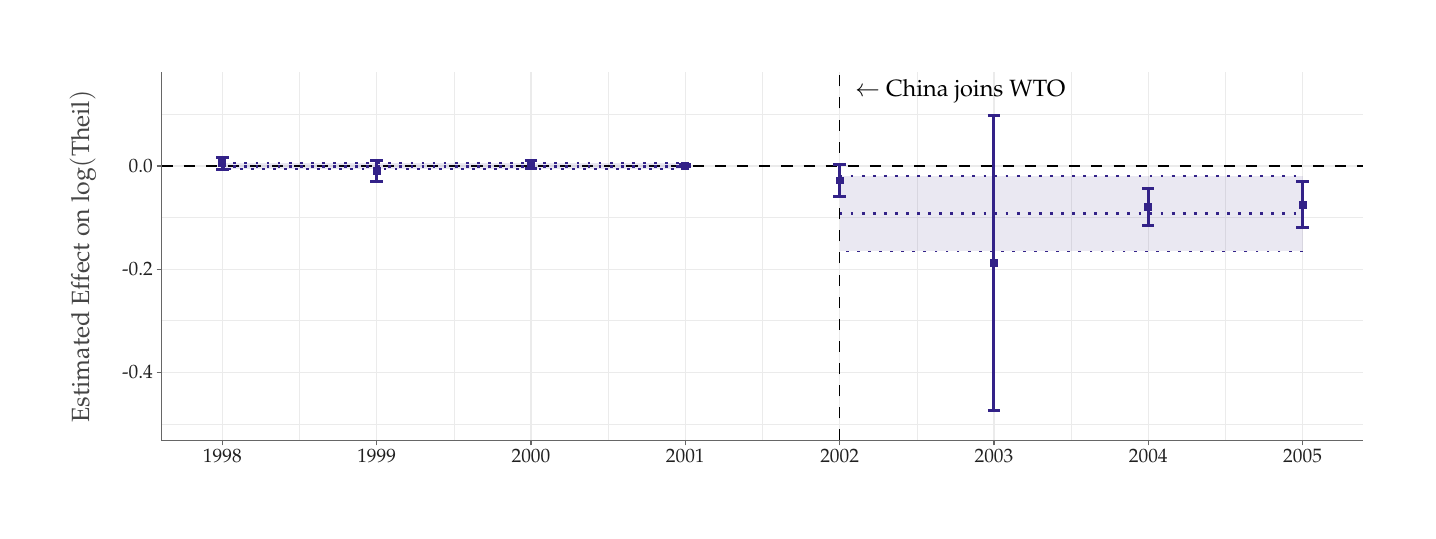
\begin{tikzpicture}[x=1pt,y=1pt]
\definecolor{fillColor}{RGB}{255,255,255}
\path[use as bounding box,fill=fillColor,fill opacity=0.00] (0,0) rectangle (498.66,174.53);
\begin{scope}
\path[clip] (  0.00,  0.00) rectangle (498.66,174.53);
\definecolor{fillColor}{RGB}{255,255,255}

\path[fill=fillColor] (  0.00,  0.00) rectangle (498.66,174.53);
\end{scope}
\begin{scope}
\path[clip] ( 48.37, 25.33) rectangle (482.66,158.53);
\definecolor{fillColor}{RGB}{255,255,255}

\path[fill=fillColor] ( 48.37, 25.33) rectangle (482.66,158.53);
\definecolor{drawColor}{gray}{0.92}

\path[draw=drawColor,line width= 0.2pt,line join=round] ( 48.37, 31.39) --
	(482.66, 31.39);

\path[draw=drawColor,line width= 0.2pt,line join=round] ( 48.37, 68.65) --
	(482.66, 68.65);

\path[draw=drawColor,line width= 0.2pt,line join=round] ( 48.37,105.90) --
	(482.66,105.90);

\path[draw=drawColor,line width= 0.2pt,line join=round] ( 48.37,143.16) --
	(482.66,143.16);

\path[draw=drawColor,line width= 0.2pt,line join=round] ( 98.22, 25.33) --
	( 98.22,158.53);

\path[draw=drawColor,line width= 0.2pt,line join=round] (153.99, 25.33) --
	(153.99,158.53);

\path[draw=drawColor,line width= 0.2pt,line join=round] (209.75, 25.33) --
	(209.75,158.53);

\path[draw=drawColor,line width= 0.2pt,line join=round] (265.52, 25.33) --
	(265.52,158.53);

\path[draw=drawColor,line width= 0.2pt,line join=round] (321.28, 25.33) --
	(321.28,158.53);

\path[draw=drawColor,line width= 0.2pt,line join=round] (377.04, 25.33) --
	(377.04,158.53);

\path[draw=drawColor,line width= 0.2pt,line join=round] (432.81, 25.33) --
	(432.81,158.53);

\path[draw=drawColor,line width= 0.4pt,line join=round] ( 48.37, 50.02) --
	(482.66, 50.02);

\path[draw=drawColor,line width= 0.4pt,line join=round] ( 48.37, 87.27) --
	(482.66, 87.27);

\path[draw=drawColor,line width= 0.4pt,line join=round] ( 48.37,124.53) --
	(482.66,124.53);

\path[draw=drawColor,line width= 0.4pt,line join=round] ( 70.34, 25.33) --
	( 70.34,158.53);

\path[draw=drawColor,line width= 0.4pt,line join=round] (126.10, 25.33) --
	(126.10,158.53);

\path[draw=drawColor,line width= 0.4pt,line join=round] (181.87, 25.33) --
	(181.87,158.53);

\path[draw=drawColor,line width= 0.4pt,line join=round] (237.63, 25.33) --
	(237.63,158.53);

\path[draw=drawColor,line width= 0.4pt,line join=round] (293.40, 25.33) --
	(293.40,158.53);

\path[draw=drawColor,line width= 0.4pt,line join=round] (349.16, 25.33) --
	(349.16,158.53);

\path[draw=drawColor,line width= 0.4pt,line join=round] (404.93, 25.33) --
	(404.93,158.53);

\path[draw=drawColor,line width= 0.4pt,line join=round] (460.69, 25.33) --
	(460.69,158.53);
\definecolor{drawColor}{RGB}{0,0,0}

\path[draw=drawColor,line width= 0.6pt,dash pattern=on 4pt off 4pt ,line join=round] ( 48.37,124.53) -- (482.66,124.53);

\path[draw=drawColor,line width= 0.6pt,dash pattern=on 4pt off 4pt ,line join=round] (293.40, 25.33) -- (293.40,158.53);

\node[text=drawColor,anchor=base west,inner sep=0pt, outer sep=0pt, scale=  0.85] at (298.97,149.54) {$\leftarrow$ China joins WTO};
\definecolor{drawColor}{RGB}{51,34,136}

\path[draw=drawColor,line width= 1.1pt,line join=round] ( 68.11,127.69) --
	( 72.57,127.69);

\path[draw=drawColor,line width= 1.1pt,line join=round] ( 70.34,127.69) --
	( 70.34,123.35);

\path[draw=drawColor,line width= 1.1pt,line join=round] ( 68.11,123.35) --
	( 72.57,123.35);

\path[draw=drawColor,line width= 1.1pt,line join=round] (123.87,126.67) --
	(128.34,126.67);

\path[draw=drawColor,line width= 1.1pt,line join=round] (126.10,126.67) --
	(126.10,118.83);

\path[draw=drawColor,line width= 1.1pt,line join=round] (123.87,118.83) --
	(128.34,118.83);

\path[draw=drawColor,line width= 1.1pt,line join=round] (179.64,126.65) --
	(184.10,126.65);

\path[draw=drawColor,line width= 1.1pt,line join=round] (181.87,126.65) --
	(181.87,123.74);

\path[draw=drawColor,line width= 1.1pt,line join=round] (179.64,123.74) --
	(184.10,123.74);

\path[draw=drawColor,line width= 1.1pt,line join=round] (235.40,124.96) --
	(239.86,124.96);

\path[draw=drawColor,line width= 1.1pt,line join=round] (237.63,124.96) --
	(237.63,124.37);

\path[draw=drawColor,line width= 1.1pt,line join=round] (235.40,124.37) --
	(239.86,124.37);

\path[draw=drawColor,line width= 1.1pt,line join=round] (291.17,124.99) --
	(295.63,124.99);

\path[draw=drawColor,line width= 1.1pt,line join=round] (293.40,124.99) --
	(293.40,113.62);

\path[draw=drawColor,line width= 1.1pt,line join=round] (291.17,113.62) --
	(295.63,113.62);

\path[draw=drawColor,line width= 1.1pt,line join=round] (346.93,142.90) --
	(351.39,142.90);

\path[draw=drawColor,line width= 1.1pt,line join=round] (349.16,142.90) --
	(349.16, 36.36);

\path[draw=drawColor,line width= 1.1pt,line join=round] (346.93, 36.36) --
	(351.39, 36.36);

\path[draw=drawColor,line width= 1.1pt,line join=round] (402.70,116.39) --
	(407.16,116.39);

\path[draw=drawColor,line width= 1.1pt,line join=round] (404.93,116.39) --
	(404.93,103.10);

\path[draw=drawColor,line width= 1.1pt,line join=round] (402.70,103.10) --
	(407.16,103.10);

\path[draw=drawColor,line width= 1.1pt,line join=round] (458.46,118.95) --
	(462.92,118.95);

\path[draw=drawColor,line width= 1.1pt,line join=round] (460.69,118.95) --
	(460.69,102.22);

\path[draw=drawColor,line width= 1.1pt,line join=round] (458.46,102.22) --
	(462.92,102.22);
\definecolor{fillColor}{RGB}{51,34,136}

\path[fill=fillColor] ( 68.91,124.09) --
	( 71.77,124.09) --
	( 71.77,126.95) --
	( 68.91,126.95) --
	cycle;

\path[fill=fillColor] (124.68,121.32) --
	(127.53,121.32) --
	(127.53,124.18) --
	(124.68,124.18) --
	cycle;

\path[fill=fillColor] (180.44,123.77) --
	(183.30,123.77) --
	(183.30,126.62) --
	(180.44,126.62) --
	cycle;

\path[fill=fillColor] (236.21,123.24) --
	(239.06,123.24) --
	(239.06,126.09) --
	(236.21,126.09) --
	cycle;

\path[fill=fillColor] (291.97,117.88) --
	(294.82,117.88) --
	(294.82,120.73) --
	(291.97,120.73) --
	cycle;

\path[fill=fillColor] (347.74, 88.21) --
	(350.59, 88.21) --
	(350.59, 91.06) --
	(347.74, 91.06) --
	cycle;

\path[fill=fillColor] (403.50,108.32) --
	(406.35,108.32) --
	(406.35,111.17) --
	(403.50,111.17) --
	cycle;

\path[fill=fillColor] (459.27,109.16) --
	(462.12,109.16) --
	(462.12,112.01) --
	(459.27,112.01) --
	cycle;
\definecolor{fillColor}{RGB}{51,34,136}

\path[fill=fillColor,fill opacity=0.10] (293.40,120.96) --
	(460.69,120.96) --
	(460.69, 93.67) --
	(293.40, 93.67) --
	cycle;

\path[draw=drawColor,line width= 0.6pt,dash pattern=on 1pt off 3pt ,line join=round] (293.40,120.96) --
	(460.69,120.96);

\path[draw=drawColor,line width= 0.6pt,dash pattern=on 1pt off 3pt ,line join=round] (460.69, 93.67) --
	(293.40, 93.67);

\path[fill=fillColor,fill opacity=0.10] ( 70.34,125.71) --
	(237.63,125.71) --
	(237.63,123.35) --
	( 70.34,123.35) --
	cycle;

\path[draw=drawColor,line width= 0.6pt,dash pattern=on 1pt off 3pt ,line join=round] ( 70.34,125.71) --
	(237.63,125.71);

\path[draw=drawColor,line width= 0.6pt,dash pattern=on 1pt off 3pt ,line join=round] (237.63,123.35) --
	( 70.34,123.35);

\path[draw=drawColor,line width= 1.1pt,dash pattern=on 1pt off 3pt ,line join=round] (293.40,107.32) --
	(460.69,107.32);

\path[draw=drawColor,line width= 1.1pt,dash pattern=on 1pt off 3pt ,line join=round] ( 70.34,124.53) --
	(237.63,124.53);
\end{scope}
\begin{scope}
\path[clip] (  0.00,  0.00) rectangle (498.66,174.53);
\definecolor{drawColor}{gray}{0.40}

\path[draw=drawColor,line width= 0.4pt,line join=round] ( 48.37, 25.33) --
	( 48.37,158.53);
\end{scope}
\begin{scope}
\path[clip] (  0.00,  0.00) rectangle (498.66,174.53);
\definecolor{drawColor}{gray}{0.13}

\node[text=drawColor,anchor=base east,inner sep=0pt, outer sep=0pt, scale=  0.70] at ( 45.22, 47.61) {-0.4};

\node[text=drawColor,anchor=base east,inner sep=0pt, outer sep=0pt, scale=  0.70] at ( 45.22, 84.86) {-0.2};

\node[text=drawColor,anchor=base east,inner sep=0pt, outer sep=0pt, scale=  0.70] at ( 45.22,122.12) {0.0};
\end{scope}
\begin{scope}
\path[clip] (  0.00,  0.00) rectangle (498.66,174.53);
\definecolor{drawColor}{gray}{0.40}

\path[draw=drawColor,line width= 0.4pt,line join=round] ( 46.62, 50.02) --
	( 48.37, 50.02);

\path[draw=drawColor,line width= 0.4pt,line join=round] ( 46.62, 87.27) --
	( 48.37, 87.27);

\path[draw=drawColor,line width= 0.4pt,line join=round] ( 46.62,124.53) --
	( 48.37,124.53);
\end{scope}
\begin{scope}
\path[clip] (  0.00,  0.00) rectangle (498.66,174.53);
\definecolor{drawColor}{gray}{0.40}

\path[draw=drawColor,line width= 0.4pt,line join=round] ( 48.37, 25.33) --
	(482.66, 25.33);
\end{scope}
\begin{scope}
\path[clip] (  0.00,  0.00) rectangle (498.66,174.53);
\definecolor{drawColor}{gray}{0.40}

\path[draw=drawColor,line width= 0.4pt,line join=round] ( 70.34, 23.58) --
	( 70.34, 25.33);

\path[draw=drawColor,line width= 0.4pt,line join=round] (126.10, 23.58) --
	(126.10, 25.33);

\path[draw=drawColor,line width= 0.4pt,line join=round] (181.87, 23.58) --
	(181.87, 25.33);

\path[draw=drawColor,line width= 0.4pt,line join=round] (237.63, 23.58) --
	(237.63, 25.33);

\path[draw=drawColor,line width= 0.4pt,line join=round] (293.40, 23.58) --
	(293.40, 25.33);

\path[draw=drawColor,line width= 0.4pt,line join=round] (349.16, 23.58) --
	(349.16, 25.33);

\path[draw=drawColor,line width= 0.4pt,line join=round] (404.93, 23.58) --
	(404.93, 25.33);

\path[draw=drawColor,line width= 0.4pt,line join=round] (460.69, 23.58) --
	(460.69, 25.33);
\end{scope}
\begin{scope}
\path[clip] (  0.00,  0.00) rectangle (498.66,174.53);
\definecolor{drawColor}{gray}{0.13}

\node[text=drawColor,anchor=base,inner sep=0pt, outer sep=0pt, scale=  0.70] at ( 70.34, 17.36) {1998};

\node[text=drawColor,anchor=base,inner sep=0pt, outer sep=0pt, scale=  0.70] at (126.10, 17.36) {1999};

\node[text=drawColor,anchor=base,inner sep=0pt, outer sep=0pt, scale=  0.70] at (181.87, 17.36) {2000};

\node[text=drawColor,anchor=base,inner sep=0pt, outer sep=0pt, scale=  0.70] at (237.63, 17.36) {2001};

\node[text=drawColor,anchor=base,inner sep=0pt, outer sep=0pt, scale=  0.70] at (293.40, 17.36) {2002};

\node[text=drawColor,anchor=base,inner sep=0pt, outer sep=0pt, scale=  0.70] at (349.16, 17.36) {2003};

\node[text=drawColor,anchor=base,inner sep=0pt, outer sep=0pt, scale=  0.70] at (404.93, 17.36) {2004};

\node[text=drawColor,anchor=base,inner sep=0pt, outer sep=0pt, scale=  0.70] at (460.69, 17.36) {2005};
\end{scope}
\begin{scope}
\path[clip] (  0.00,  0.00) rectangle (498.66,174.53);
\definecolor{drawColor}{gray}{0.27}

\node[text=drawColor,rotate= 90.00,anchor=base,inner sep=0pt, outer sep=0pt, scale=  0.90] at ( 22.20, 91.93) {Estimated Effect on $\log($Theil$)$};
\end{scope}
\end{tikzpicture}

    \end{subfigure}
    
    \begin{subfigure}[b]{\textwidth}
        \caption{Mediated Effect via TFP Dispersion}
        % Created by tikzDevice version 0.12.3.1 on 2023-05-05 12:22:56
% !TEX encoding = UTF-8 Unicode
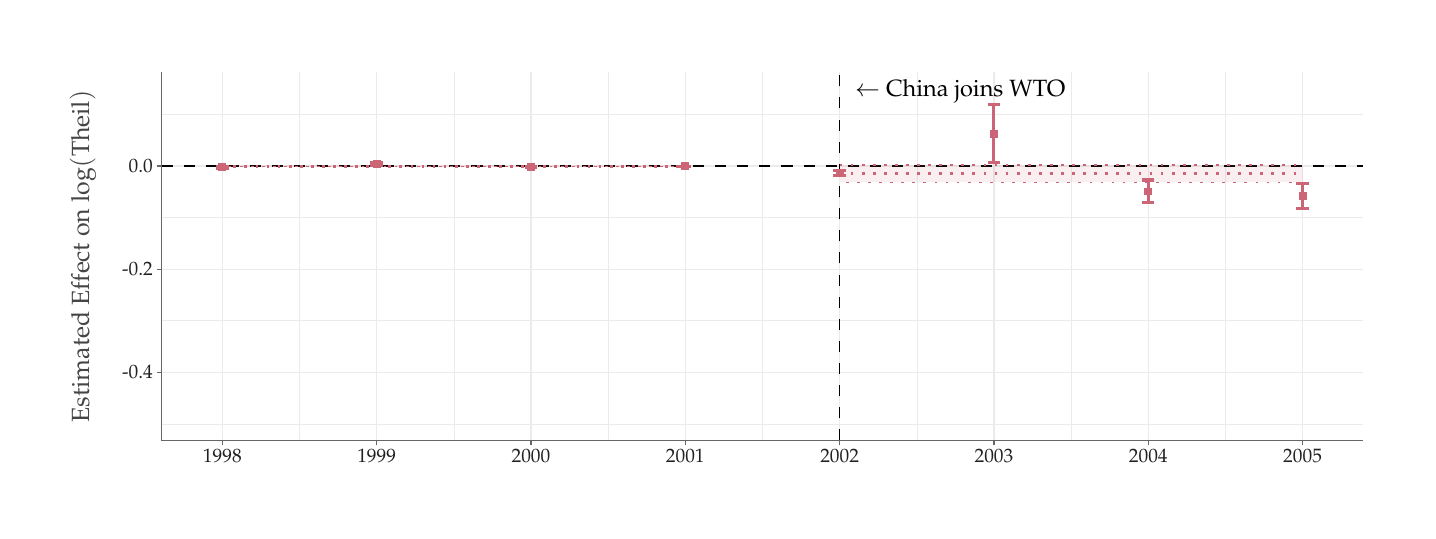
\begin{tikzpicture}[x=1pt,y=1pt]
\definecolor{fillColor}{RGB}{255,255,255}
\path[use as bounding box,fill=fillColor,fill opacity=0.00] (0,0) rectangle (498.66,174.53);
\begin{scope}
\path[clip] (  0.00,  0.00) rectangle (498.66,174.53);
\definecolor{fillColor}{RGB}{255,255,255}

\path[fill=fillColor] (  0.00,  0.00) rectangle (498.66,174.53);
\end{scope}
\begin{scope}
\path[clip] ( 48.37, 25.33) rectangle (482.66,158.53);
\definecolor{fillColor}{RGB}{255,255,255}

\path[fill=fillColor] ( 48.37, 25.33) rectangle (482.66,158.53);
\definecolor{drawColor}{gray}{0.92}

\path[draw=drawColor,line width= 0.2pt,line join=round] ( 48.37, 31.39) --
	(482.66, 31.39);

\path[draw=drawColor,line width= 0.2pt,line join=round] ( 48.37, 68.65) --
	(482.66, 68.65);

\path[draw=drawColor,line width= 0.2pt,line join=round] ( 48.37,105.90) --
	(482.66,105.90);

\path[draw=drawColor,line width= 0.2pt,line join=round] ( 48.37,143.16) --
	(482.66,143.16);

\path[draw=drawColor,line width= 0.2pt,line join=round] ( 98.22, 25.33) --
	( 98.22,158.53);

\path[draw=drawColor,line width= 0.2pt,line join=round] (153.99, 25.33) --
	(153.99,158.53);

\path[draw=drawColor,line width= 0.2pt,line join=round] (209.75, 25.33) --
	(209.75,158.53);

\path[draw=drawColor,line width= 0.2pt,line join=round] (265.52, 25.33) --
	(265.52,158.53);

\path[draw=drawColor,line width= 0.2pt,line join=round] (321.28, 25.33) --
	(321.28,158.53);

\path[draw=drawColor,line width= 0.2pt,line join=round] (377.04, 25.33) --
	(377.04,158.53);

\path[draw=drawColor,line width= 0.2pt,line join=round] (432.81, 25.33) --
	(432.81,158.53);

\path[draw=drawColor,line width= 0.4pt,line join=round] ( 48.37, 50.02) --
	(482.66, 50.02);

\path[draw=drawColor,line width= 0.4pt,line join=round] ( 48.37, 87.27) --
	(482.66, 87.27);

\path[draw=drawColor,line width= 0.4pt,line join=round] ( 48.37,124.53) --
	(482.66,124.53);

\path[draw=drawColor,line width= 0.4pt,line join=round] ( 70.34, 25.33) --
	( 70.34,158.53);

\path[draw=drawColor,line width= 0.4pt,line join=round] (126.10, 25.33) --
	(126.10,158.53);

\path[draw=drawColor,line width= 0.4pt,line join=round] (181.87, 25.33) --
	(181.87,158.53);

\path[draw=drawColor,line width= 0.4pt,line join=round] (237.63, 25.33) --
	(237.63,158.53);

\path[draw=drawColor,line width= 0.4pt,line join=round] (293.40, 25.33) --
	(293.40,158.53);

\path[draw=drawColor,line width= 0.4pt,line join=round] (349.16, 25.33) --
	(349.16,158.53);

\path[draw=drawColor,line width= 0.4pt,line join=round] (404.93, 25.33) --
	(404.93,158.53);

\path[draw=drawColor,line width= 0.4pt,line join=round] (460.69, 25.33) --
	(460.69,158.53);
\definecolor{drawColor}{RGB}{0,0,0}

\path[draw=drawColor,line width= 0.6pt,dash pattern=on 4pt off 4pt ,line join=round] ( 48.37,124.53) -- (482.66,124.53);

\path[draw=drawColor,line width= 0.6pt,dash pattern=on 4pt off 4pt ,line join=round] (293.40, 25.33) -- (293.40,158.53);

\node[text=drawColor,anchor=base west,inner sep=0pt, outer sep=0pt, scale=  0.85] at (298.97,149.54) {$\leftarrow$ China joins WTO};
\definecolor{drawColor}{RGB}{204,102,119}

\path[draw=drawColor,line width= 1.1pt,line join=round] ( 68.11,124.48) --
	( 72.57,124.48);

\path[draw=drawColor,line width= 1.1pt,line join=round] ( 70.34,124.48) --
	( 70.34,123.78);

\path[draw=drawColor,line width= 1.1pt,line join=round] ( 68.11,123.78) --
	( 72.57,123.78);

\path[draw=drawColor,line width= 1.1pt,line join=round] (123.87,125.90) --
	(128.34,125.90);

\path[draw=drawColor,line width= 1.1pt,line join=round] (126.10,125.90) --
	(126.10,124.64);

\path[draw=drawColor,line width= 1.1pt,line join=round] (123.87,124.64) --
	(128.34,124.64);

\path[draw=drawColor,line width= 1.1pt,line join=round] (179.64,124.49) --
	(184.10,124.49);

\path[draw=drawColor,line width= 1.1pt,line join=round] (181.87,124.49) --
	(181.87,124.03);

\path[draw=drawColor,line width= 1.1pt,line join=round] (179.64,124.03) --
	(184.10,124.03);

\path[draw=drawColor,line width= 1.1pt,line join=round] (235.40,124.53) --
	(239.86,124.53);

\path[draw=drawColor,line width= 1.1pt,line join=round] (237.63,124.53) --
	(237.63,124.43);

\path[draw=drawColor,line width= 1.1pt,line join=round] (235.40,124.43) --
	(239.86,124.43);

\path[draw=drawColor,line width= 1.1pt,line join=round] (291.17,122.86) --
	(295.63,122.86);

\path[draw=drawColor,line width= 1.1pt,line join=round] (293.40,122.86) --
	(293.40,121.04);

\path[draw=drawColor,line width= 1.1pt,line join=round] (291.17,121.04) --
	(295.63,121.04);

\path[draw=drawColor,line width= 1.1pt,line join=round] (346.93,146.71) --
	(351.39,146.71);

\path[draw=drawColor,line width= 1.1pt,line join=round] (349.16,146.71) --
	(349.16,125.75);

\path[draw=drawColor,line width= 1.1pt,line join=round] (346.93,125.75) --
	(351.39,125.75);

\path[draw=drawColor,line width= 1.1pt,line join=round] (402.70,119.48) --
	(407.16,119.48);

\path[draw=drawColor,line width= 1.1pt,line join=round] (404.93,119.48) --
	(404.93,111.19);

\path[draw=drawColor,line width= 1.1pt,line join=round] (402.70,111.19) --
	(407.16,111.19);

\path[draw=drawColor,line width= 1.1pt,line join=round] (458.46,118.36) --
	(462.92,118.36);

\path[draw=drawColor,line width= 1.1pt,line join=round] (460.69,118.36) --
	(460.69,109.08);

\path[draw=drawColor,line width= 1.1pt,line join=round] (458.46,109.08) --
	(462.92,109.08);
\definecolor{fillColor}{RGB}{204,102,119}

\path[fill=fillColor] ( 68.91,122.70) --
	( 71.77,122.70) --
	( 71.77,125.55) --
	( 68.91,125.55) --
	cycle;

\path[fill=fillColor] (124.68,123.84) --
	(127.53,123.84) --
	(127.53,126.70) --
	(124.68,126.70) --
	cycle;

\path[fill=fillColor] (180.44,122.83) --
	(183.30,122.83) --
	(183.30,125.69) --
	(180.44,125.69) --
	cycle;

\path[fill=fillColor] (236.21,123.05) --
	(239.06,123.05) --
	(239.06,125.90) --
	(236.21,125.90) --
	cycle;

\path[fill=fillColor] (291.97,120.52) --
	(294.82,120.52) --
	(294.82,123.37) --
	(291.97,123.37) --
	cycle;

\path[fill=fillColor] (347.74,134.81) --
	(350.59,134.81) --
	(350.59,137.66) --
	(347.74,137.66) --
	cycle;

\path[fill=fillColor] (403.50,113.91) --
	(406.35,113.91) --
	(406.35,116.76) --
	(403.50,116.76) --
	cycle;

\path[fill=fillColor] (459.27,112.29) --
	(462.12,112.29) --
	(462.12,115.14) --
	(459.27,115.14) --
	cycle;
\definecolor{fillColor}{RGB}{204,102,119}

\path[fill=fillColor,fill opacity=0.10] (293.40,125.01) --
	(460.69,125.01) --
	(460.69,118.60) --
	(293.40,118.60) --
	cycle;

\path[draw=drawColor,line width= 0.6pt,dash pattern=on 1pt off 3pt ,line join=round] (293.40,125.01) --
	(460.69,125.01);

\path[draw=drawColor,line width= 0.6pt,dash pattern=on 1pt off 3pt ,line join=round] (460.69,118.60) --
	(293.40,118.60);

\path[fill=fillColor,fill opacity=0.10] ( 70.34,124.73) --
	(237.63,124.73) --
	(237.63,124.34) --
	( 70.34,124.34) --
	cycle;

\path[draw=drawColor,line width= 0.6pt,dash pattern=on 1pt off 3pt ,line join=round] ( 70.34,124.73) --
	(237.63,124.73);

\path[draw=drawColor,line width= 0.6pt,dash pattern=on 1pt off 3pt ,line join=round] (237.63,124.34) --
	( 70.34,124.34);

\path[draw=drawColor,line width= 1.1pt,dash pattern=on 1pt off 3pt ,line join=round] (293.40,121.81) --
	(460.69,121.81);

\path[draw=drawColor,line width= 1.1pt,dash pattern=on 1pt off 3pt ,line join=round] ( 70.34,124.53) --
	(237.63,124.53);
\end{scope}
\begin{scope}
\path[clip] (  0.00,  0.00) rectangle (498.66,174.53);
\definecolor{drawColor}{gray}{0.40}

\path[draw=drawColor,line width= 0.4pt,line join=round] ( 48.37, 25.33) --
	( 48.37,158.53);
\end{scope}
\begin{scope}
\path[clip] (  0.00,  0.00) rectangle (498.66,174.53);
\definecolor{drawColor}{gray}{0.13}

\node[text=drawColor,anchor=base east,inner sep=0pt, outer sep=0pt, scale=  0.70] at ( 45.22, 47.61) {-0.4};

\node[text=drawColor,anchor=base east,inner sep=0pt, outer sep=0pt, scale=  0.70] at ( 45.22, 84.86) {-0.2};

\node[text=drawColor,anchor=base east,inner sep=0pt, outer sep=0pt, scale=  0.70] at ( 45.22,122.12) {0.0};
\end{scope}
\begin{scope}
\path[clip] (  0.00,  0.00) rectangle (498.66,174.53);
\definecolor{drawColor}{gray}{0.40}

\path[draw=drawColor,line width= 0.4pt,line join=round] ( 46.62, 50.02) --
	( 48.37, 50.02);

\path[draw=drawColor,line width= 0.4pt,line join=round] ( 46.62, 87.27) --
	( 48.37, 87.27);

\path[draw=drawColor,line width= 0.4pt,line join=round] ( 46.62,124.53) --
	( 48.37,124.53);
\end{scope}
\begin{scope}
\path[clip] (  0.00,  0.00) rectangle (498.66,174.53);
\definecolor{drawColor}{gray}{0.40}

\path[draw=drawColor,line width= 0.4pt,line join=round] ( 48.37, 25.33) --
	(482.66, 25.33);
\end{scope}
\begin{scope}
\path[clip] (  0.00,  0.00) rectangle (498.66,174.53);
\definecolor{drawColor}{gray}{0.40}

\path[draw=drawColor,line width= 0.4pt,line join=round] ( 70.34, 23.58) --
	( 70.34, 25.33);

\path[draw=drawColor,line width= 0.4pt,line join=round] (126.10, 23.58) --
	(126.10, 25.33);

\path[draw=drawColor,line width= 0.4pt,line join=round] (181.87, 23.58) --
	(181.87, 25.33);

\path[draw=drawColor,line width= 0.4pt,line join=round] (237.63, 23.58) --
	(237.63, 25.33);

\path[draw=drawColor,line width= 0.4pt,line join=round] (293.40, 23.58) --
	(293.40, 25.33);

\path[draw=drawColor,line width= 0.4pt,line join=round] (349.16, 23.58) --
	(349.16, 25.33);

\path[draw=drawColor,line width= 0.4pt,line join=round] (404.93, 23.58) --
	(404.93, 25.33);

\path[draw=drawColor,line width= 0.4pt,line join=round] (460.69, 23.58) --
	(460.69, 25.33);
\end{scope}
\begin{scope}
\path[clip] (  0.00,  0.00) rectangle (498.66,174.53);
\definecolor{drawColor}{gray}{0.13}

\node[text=drawColor,anchor=base,inner sep=0pt, outer sep=0pt, scale=  0.70] at ( 70.34, 17.36) {1998};

\node[text=drawColor,anchor=base,inner sep=0pt, outer sep=0pt, scale=  0.70] at (126.10, 17.36) {1999};

\node[text=drawColor,anchor=base,inner sep=0pt, outer sep=0pt, scale=  0.70] at (181.87, 17.36) {2000};

\node[text=drawColor,anchor=base,inner sep=0pt, outer sep=0pt, scale=  0.70] at (237.63, 17.36) {2001};

\node[text=drawColor,anchor=base,inner sep=0pt, outer sep=0pt, scale=  0.70] at (293.40, 17.36) {2002};

\node[text=drawColor,anchor=base,inner sep=0pt, outer sep=0pt, scale=  0.70] at (349.16, 17.36) {2003};

\node[text=drawColor,anchor=base,inner sep=0pt, outer sep=0pt, scale=  0.70] at (404.93, 17.36) {2004};

\node[text=drawColor,anchor=base,inner sep=0pt, outer sep=0pt, scale=  0.70] at (460.69, 17.36) {2005};
\end{scope}
\begin{scope}
\path[clip] (  0.00,  0.00) rectangle (498.66,174.53);
\definecolor{drawColor}{gray}{0.27}

\node[text=drawColor,rotate= 90.00,anchor=base,inner sep=0pt, outer sep=0pt, scale=  0.90] at ( 22.20, 91.93) {Estimated Effect on $\log($Theil$)$};
\end{scope}
\end{tikzpicture}

    \end{subfigure}
    
    {\footnotesize\emph{Notes:} These figures presents event-study estimates and 95\% confidence intervals for the effect of China WTO ascension on the dispersion of firm-level markups within an industry defined by the Theil index given in (\ref{eq:theil_index}). Treatment is equal to one for industries with above-median 2001 tariff rates with China for years 2002 and beyond. Estimates are computed using the CCEDID estimator proposed in the paper with the Theil index of firm-level total factor productivity as the covariate X. A constant factor is included as an observed factor. Panel (a) presents estimates of the total effect of WTO Ascension, $\Delta$, and panel (b) presents the portion of the effect mediated by the Theil index in firm-level total factor productivity.}
\end{figure}

\begin{figure}
    \caption{China WTO Ascension and Markup Dispersion (with 2003 Interpolated)}
    \label{fig:trade_interpolation}

    \begin{subfigure}[b]{\textwidth}
        \caption{Total Effect}
        % Created by tikzDevice version 0.12.3.1 on 2023-05-05 12:23:03
% !TEX encoding = UTF-8 Unicode
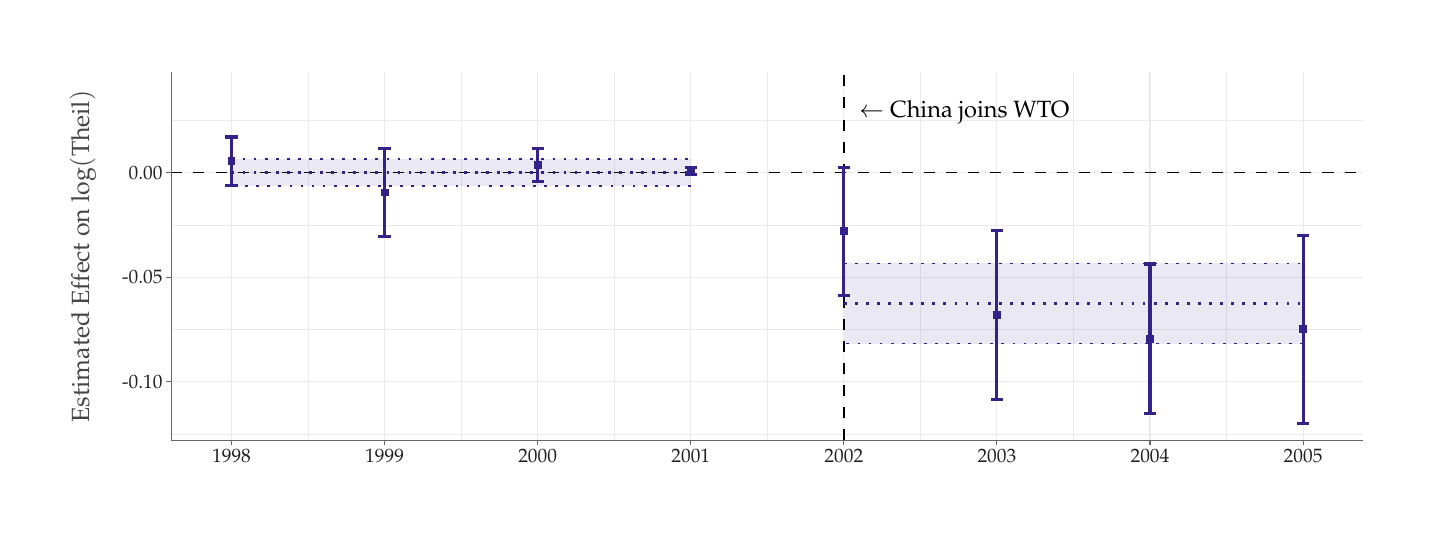
\begin{tikzpicture}[x=1pt,y=1pt]
\definecolor{fillColor}{RGB}{255,255,255}
\path[use as bounding box,fill=fillColor,fill opacity=0.00] (0,0) rectangle (498.66,174.53);
\begin{scope}
\path[clip] (  0.00,  0.00) rectangle (498.66,174.53);
\definecolor{fillColor}{RGB}{255,255,255}

\path[fill=fillColor] (  0.00,  0.00) rectangle (498.66,174.53);
\end{scope}
\begin{scope}
\path[clip] ( 51.87, 25.33) rectangle (482.66,158.53);
\definecolor{fillColor}{RGB}{255,255,255}

\path[fill=fillColor] ( 51.87, 25.33) rectangle (482.66,158.53);
\definecolor{drawColor}{gray}{0.92}

\path[draw=drawColor,line width= 0.2pt,line join=round] ( 51.87, 27.60) --
	(482.66, 27.60);

\path[draw=drawColor,line width= 0.2pt,line join=round] ( 51.87, 65.44) --
	(482.66, 65.44);

\path[draw=drawColor,line width= 0.2pt,line join=round] ( 51.87,103.28) --
	(482.66,103.28);

\path[draw=drawColor,line width= 0.2pt,line join=round] ( 51.87,141.13) --
	(482.66,141.13);

\path[draw=drawColor,line width= 0.2pt,line join=round] (101.32, 25.33) --
	(101.32,158.53);

\path[draw=drawColor,line width= 0.2pt,line join=round] (156.63, 25.33) --
	(156.63,158.53);

\path[draw=drawColor,line width= 0.2pt,line join=round] (211.95, 25.33) --
	(211.95,158.53);

\path[draw=drawColor,line width= 0.2pt,line join=round] (267.27, 25.33) --
	(267.27,158.53);

\path[draw=drawColor,line width= 0.2pt,line join=round] (322.58, 25.33) --
	(322.58,158.53);

\path[draw=drawColor,line width= 0.2pt,line join=round] (377.90, 25.33) --
	(377.90,158.53);

\path[draw=drawColor,line width= 0.2pt,line join=round] (433.21, 25.33) --
	(433.21,158.53);

\path[draw=drawColor,line width= 0.4pt,line join=round] ( 51.87, 46.52) --
	(482.66, 46.52);

\path[draw=drawColor,line width= 0.4pt,line join=round] ( 51.87, 84.36) --
	(482.66, 84.36);

\path[draw=drawColor,line width= 0.4pt,line join=round] ( 51.87,122.20) --
	(482.66,122.20);

\path[draw=drawColor,line width= 0.4pt,line join=round] ( 73.66, 25.33) --
	( 73.66,158.53);

\path[draw=drawColor,line width= 0.4pt,line join=round] (128.98, 25.33) --
	(128.98,158.53);

\path[draw=drawColor,line width= 0.4pt,line join=round] (184.29, 25.33) --
	(184.29,158.53);

\path[draw=drawColor,line width= 0.4pt,line join=round] (239.61, 25.33) --
	(239.61,158.53);

\path[draw=drawColor,line width= 0.4pt,line join=round] (294.92, 25.33) --
	(294.92,158.53);

\path[draw=drawColor,line width= 0.4pt,line join=round] (350.24, 25.33) --
	(350.24,158.53);

\path[draw=drawColor,line width= 0.4pt,line join=round] (405.55, 25.33) --
	(405.55,158.53);

\path[draw=drawColor,line width= 0.4pt,line join=round] (460.87, 25.33) --
	(460.87,158.53);
\definecolor{drawColor}{RGB}{0,0,0}

\path[draw=drawColor,line width= 0.6pt,dash pattern=on 4pt off 4pt ,line join=round] ( 51.87,122.20) -- (482.66,122.20);

\path[draw=drawColor,line width= 0.6pt,dash pattern=on 4pt off 4pt ,line join=round] (294.92, 25.33) -- (294.92,158.53);

\node[text=drawColor,anchor=base west,inner sep=0pt, outer sep=0pt, scale=  0.85] at (300.45,141.97) {$\leftarrow$ China joins WTO};
\definecolor{drawColor}{RGB}{51,34,136}

\path[draw=drawColor,line width= 1.1pt,line join=round] ( 71.45,135.02) --
	( 75.87,135.02);

\path[draw=drawColor,line width= 1.1pt,line join=round] ( 73.66,135.02) --
	( 73.66,117.40);

\path[draw=drawColor,line width= 1.1pt,line join=round] ( 71.45,117.40) --
	( 75.87,117.40);

\path[draw=drawColor,line width= 1.1pt,line join=round] (126.76,130.88) --
	(131.19,130.88);

\path[draw=drawColor,line width= 1.1pt,line join=round] (128.98,130.88) --
	(128.98, 99.03);

\path[draw=drawColor,line width= 1.1pt,line join=round] (126.76, 99.03) --
	(131.19, 99.03);

\path[draw=drawColor,line width= 1.1pt,line join=round] (182.08,130.81) --
	(186.51,130.81);

\path[draw=drawColor,line width= 1.1pt,line join=round] (184.29,130.81) --
	(184.29,118.98);

\path[draw=drawColor,line width= 1.1pt,line join=round] (182.08,118.98) --
	(186.51,118.98);

\path[draw=drawColor,line width= 1.1pt,line join=round] (237.40,123.95) --
	(241.82,123.95);

\path[draw=drawColor,line width= 1.1pt,line join=round] (239.61,123.95) --
	(239.61,121.55);

\path[draw=drawColor,line width= 1.1pt,line join=round] (237.40,121.55) --
	(241.82,121.55);

\path[draw=drawColor,line width= 1.1pt,line join=round] (292.71,124.06) --
	(297.14,124.06);

\path[draw=drawColor,line width= 1.1pt,line join=round] (294.92,124.06) --
	(294.92, 77.87);

\path[draw=drawColor,line width= 1.1pt,line join=round] (292.71, 77.87) --
	(297.14, 77.87);

\path[draw=drawColor,line width= 1.1pt,line join=round] (348.03,101.32) --
	(352.45,101.32);

\path[draw=drawColor,line width= 1.1pt,line join=round] (350.24,101.32) --
	(350.24, 40.20);

\path[draw=drawColor,line width= 1.1pt,line join=round] (348.03, 40.20) --
	(352.45, 40.20);

\path[draw=drawColor,line width= 1.1pt,line join=round] (403.34, 89.13) --
	(407.77, 89.13);

\path[draw=drawColor,line width= 1.1pt,line join=round] (405.55, 89.13) --
	(405.55, 35.14);

\path[draw=drawColor,line width= 1.1pt,line join=round] (403.34, 35.14) --
	(407.77, 35.14);

\path[draw=drawColor,line width= 1.1pt,line join=round] (458.66, 99.53) --
	(463.08, 99.53);

\path[draw=drawColor,line width= 1.1pt,line join=round] (460.87, 99.53) --
	(460.87, 31.57);

\path[draw=drawColor,line width= 1.1pt,line join=round] (458.66, 31.57) --
	(463.08, 31.57);
\definecolor{fillColor}{RGB}{51,34,136}

\path[fill=fillColor] ( 72.24,124.79) --
	( 75.09,124.79) --
	( 75.09,127.64) --
	( 72.24,127.64) --
	cycle;

\path[fill=fillColor] (127.55,113.53) --
	(130.40,113.53) --
	(130.40,116.39) --
	(127.55,116.39) --
	cycle;

\path[fill=fillColor] (182.87,123.47) --
	(185.72,123.47) --
	(185.72,126.32) --
	(182.87,126.32) --
	cycle;

\path[fill=fillColor] (238.18,121.32) --
	(241.03,121.32) --
	(241.03,124.18) --
	(238.18,124.18) --
	cycle;

\path[fill=fillColor] (293.50, 99.54) --
	(296.35, 99.54) --
	(296.35,102.40) --
	(293.50,102.40) --
	cycle;

\path[fill=fillColor] (348.81, 69.33) --
	(351.66, 69.33) --
	(351.66, 72.19) --
	(348.81, 72.19) --
	cycle;

\path[fill=fillColor] (404.13, 60.70) --
	(406.98, 60.70) --
	(406.98, 63.56) --
	(404.13, 63.56) --
	cycle;

\path[fill=fillColor] (459.44, 64.12) --
	(462.30, 64.12) --
	(462.30, 66.97) --
	(459.44, 66.97) --
	cycle;
\definecolor{fillColor}{RGB}{51,34,136}

\path[fill=fillColor,fill opacity=0.10] (294.92, 89.36) --
	(460.87, 89.36) --
	(460.87, 60.35) --
	(294.92, 60.35) --
	cycle;

\path[draw=drawColor,line width= 0.6pt,dash pattern=on 1pt off 3pt ,line join=round] (294.92, 89.36) --
	(460.87, 89.36);

\path[draw=drawColor,line width= 0.6pt,dash pattern=on 1pt off 3pt ,line join=round] (460.87, 60.35) --
	(294.92, 60.35);

\path[fill=fillColor,fill opacity=0.10] ( 73.66,127.00) --
	(239.61,127.00) --
	(239.61,117.41) --
	( 73.66,117.41) --
	cycle;

\path[draw=drawColor,line width= 0.6pt,dash pattern=on 1pt off 3pt ,line join=round] ( 73.66,127.00) --
	(239.61,127.00);

\path[draw=drawColor,line width= 0.6pt,dash pattern=on 1pt off 3pt ,line join=round] (239.61,117.41) --
	( 73.66,117.41);

\path[draw=drawColor,line width= 1.1pt,dash pattern=on 1pt off 3pt ,line join=round] (294.92, 74.85) --
	(460.87, 74.85);

\path[draw=drawColor,line width= 1.1pt,dash pattern=on 1pt off 3pt ,line join=round] ( 73.66,122.20) --
	(239.61,122.20);
\end{scope}
\begin{scope}
\path[clip] (  0.00,  0.00) rectangle (498.66,174.53);
\definecolor{drawColor}{gray}{0.40}

\path[draw=drawColor,line width= 0.4pt,line join=round] ( 51.87, 25.33) --
	( 51.87,158.53);
\end{scope}
\begin{scope}
\path[clip] (  0.00,  0.00) rectangle (498.66,174.53);
\definecolor{drawColor}{gray}{0.13}

\node[text=drawColor,anchor=base east,inner sep=0pt, outer sep=0pt, scale=  0.70] at ( 48.72, 44.11) {-0.10};

\node[text=drawColor,anchor=base east,inner sep=0pt, outer sep=0pt, scale=  0.70] at ( 48.72, 81.95) {-0.05};

\node[text=drawColor,anchor=base east,inner sep=0pt, outer sep=0pt, scale=  0.70] at ( 48.72,119.79) {0.00};
\end{scope}
\begin{scope}
\path[clip] (  0.00,  0.00) rectangle (498.66,174.53);
\definecolor{drawColor}{gray}{0.40}

\path[draw=drawColor,line width= 0.4pt,line join=round] ( 50.12, 46.52) --
	( 51.87, 46.52);

\path[draw=drawColor,line width= 0.4pt,line join=round] ( 50.12, 84.36) --
	( 51.87, 84.36);

\path[draw=drawColor,line width= 0.4pt,line join=round] ( 50.12,122.20) --
	( 51.87,122.20);
\end{scope}
\begin{scope}
\path[clip] (  0.00,  0.00) rectangle (498.66,174.53);
\definecolor{drawColor}{gray}{0.40}

\path[draw=drawColor,line width= 0.4pt,line join=round] ( 51.87, 25.33) --
	(482.66, 25.33);
\end{scope}
\begin{scope}
\path[clip] (  0.00,  0.00) rectangle (498.66,174.53);
\definecolor{drawColor}{gray}{0.40}

\path[draw=drawColor,line width= 0.4pt,line join=round] ( 73.66, 23.58) --
	( 73.66, 25.33);

\path[draw=drawColor,line width= 0.4pt,line join=round] (128.98, 23.58) --
	(128.98, 25.33);

\path[draw=drawColor,line width= 0.4pt,line join=round] (184.29, 23.58) --
	(184.29, 25.33);

\path[draw=drawColor,line width= 0.4pt,line join=round] (239.61, 23.58) --
	(239.61, 25.33);

\path[draw=drawColor,line width= 0.4pt,line join=round] (294.92, 23.58) --
	(294.92, 25.33);

\path[draw=drawColor,line width= 0.4pt,line join=round] (350.24, 23.58) --
	(350.24, 25.33);

\path[draw=drawColor,line width= 0.4pt,line join=round] (405.55, 23.58) --
	(405.55, 25.33);

\path[draw=drawColor,line width= 0.4pt,line join=round] (460.87, 23.58) --
	(460.87, 25.33);
\end{scope}
\begin{scope}
\path[clip] (  0.00,  0.00) rectangle (498.66,174.53);
\definecolor{drawColor}{gray}{0.13}

\node[text=drawColor,anchor=base,inner sep=0pt, outer sep=0pt, scale=  0.70] at ( 73.66, 17.36) {1998};

\node[text=drawColor,anchor=base,inner sep=0pt, outer sep=0pt, scale=  0.70] at (128.98, 17.36) {1999};

\node[text=drawColor,anchor=base,inner sep=0pt, outer sep=0pt, scale=  0.70] at (184.29, 17.36) {2000};

\node[text=drawColor,anchor=base,inner sep=0pt, outer sep=0pt, scale=  0.70] at (239.61, 17.36) {2001};

\node[text=drawColor,anchor=base,inner sep=0pt, outer sep=0pt, scale=  0.70] at (294.92, 17.36) {2002};

\node[text=drawColor,anchor=base,inner sep=0pt, outer sep=0pt, scale=  0.70] at (350.24, 17.36) {2003};

\node[text=drawColor,anchor=base,inner sep=0pt, outer sep=0pt, scale=  0.70] at (405.55, 17.36) {2004};

\node[text=drawColor,anchor=base,inner sep=0pt, outer sep=0pt, scale=  0.70] at (460.87, 17.36) {2005};
\end{scope}
\begin{scope}
\path[clip] (  0.00,  0.00) rectangle (498.66,174.53);
\definecolor{drawColor}{gray}{0.27}

\node[text=drawColor,rotate= 90.00,anchor=base,inner sep=0pt, outer sep=0pt, scale=  0.90] at ( 22.20, 91.93) {Estimated Effect on $\log($Theil$)$};
\end{scope}
\end{tikzpicture}

    \end{subfigure}
    
    \begin{subfigure}[b]{\textwidth}
        \caption{Mediated Effect via TFP Dispersion}
        % Created by tikzDevice version 0.12.3.1 on 2023-05-05 12:42:55
% !TEX encoding = UTF-8 Unicode
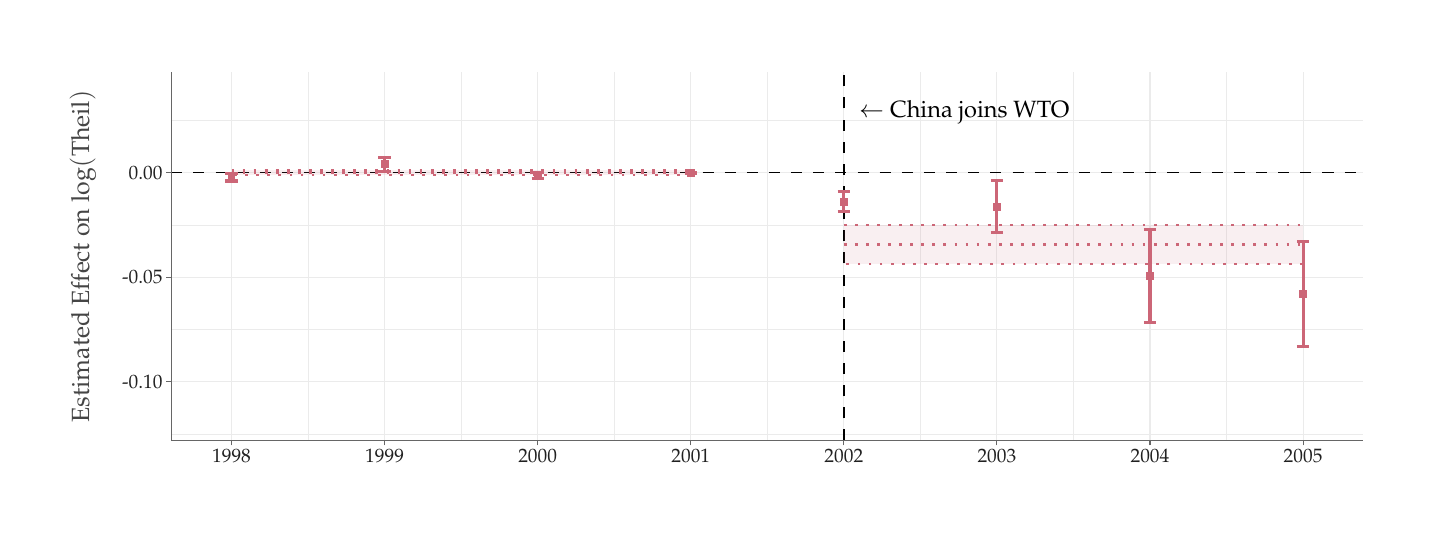
\begin{tikzpicture}[x=1pt,y=1pt]
\definecolor{fillColor}{RGB}{255,255,255}
\path[use as bounding box,fill=fillColor,fill opacity=0.00] (0,0) rectangle (498.66,174.53);
\begin{scope}
\path[clip] (  0.00,  0.00) rectangle (498.66,174.53);
\definecolor{fillColor}{RGB}{255,255,255}

\path[fill=fillColor] (  0.00,  0.00) rectangle (498.66,174.53);
\end{scope}
\begin{scope}
\path[clip] ( 51.87, 25.33) rectangle (482.66,158.53);
\definecolor{fillColor}{RGB}{255,255,255}

\path[fill=fillColor] ( 51.87, 25.33) rectangle (482.66,158.53);
\definecolor{drawColor}{gray}{0.92}

\path[draw=drawColor,line width= 0.2pt,line join=round] ( 51.87, 27.60) --
	(482.66, 27.60);

\path[draw=drawColor,line width= 0.2pt,line join=round] ( 51.87, 65.44) --
	(482.66, 65.44);

\path[draw=drawColor,line width= 0.2pt,line join=round] ( 51.87,103.28) --
	(482.66,103.28);

\path[draw=drawColor,line width= 0.2pt,line join=round] ( 51.87,141.13) --
	(482.66,141.13);

\path[draw=drawColor,line width= 0.2pt,line join=round] (101.32, 25.33) --
	(101.32,158.53);

\path[draw=drawColor,line width= 0.2pt,line join=round] (156.63, 25.33) --
	(156.63,158.53);

\path[draw=drawColor,line width= 0.2pt,line join=round] (211.95, 25.33) --
	(211.95,158.53);

\path[draw=drawColor,line width= 0.2pt,line join=round] (267.27, 25.33) --
	(267.27,158.53);

\path[draw=drawColor,line width= 0.2pt,line join=round] (322.58, 25.33) --
	(322.58,158.53);

\path[draw=drawColor,line width= 0.2pt,line join=round] (377.90, 25.33) --
	(377.90,158.53);

\path[draw=drawColor,line width= 0.2pt,line join=round] (433.21, 25.33) --
	(433.21,158.53);

\path[draw=drawColor,line width= 0.4pt,line join=round] ( 51.87, 46.52) --
	(482.66, 46.52);

\path[draw=drawColor,line width= 0.4pt,line join=round] ( 51.87, 84.36) --
	(482.66, 84.36);

\path[draw=drawColor,line width= 0.4pt,line join=round] ( 51.87,122.20) --
	(482.66,122.20);

\path[draw=drawColor,line width= 0.4pt,line join=round] ( 73.66, 25.33) --
	( 73.66,158.53);

\path[draw=drawColor,line width= 0.4pt,line join=round] (128.98, 25.33) --
	(128.98,158.53);

\path[draw=drawColor,line width= 0.4pt,line join=round] (184.29, 25.33) --
	(184.29,158.53);

\path[draw=drawColor,line width= 0.4pt,line join=round] (239.61, 25.33) --
	(239.61,158.53);

\path[draw=drawColor,line width= 0.4pt,line join=round] (294.92, 25.33) --
	(294.92,158.53);

\path[draw=drawColor,line width= 0.4pt,line join=round] (350.24, 25.33) --
	(350.24,158.53);

\path[draw=drawColor,line width= 0.4pt,line join=round] (405.55, 25.33) --
	(405.55,158.53);

\path[draw=drawColor,line width= 0.4pt,line join=round] (460.87, 25.33) --
	(460.87,158.53);
\definecolor{drawColor}{RGB}{0,0,0}

\path[draw=drawColor,line width= 0.6pt,dash pattern=on 4pt off 4pt ,line join=round] ( 51.87,122.20) -- (482.66,122.20);

\path[draw=drawColor,line width= 0.6pt,dash pattern=on 4pt off 4pt ,line join=round] (294.92, 25.33) -- (294.92,158.53);

\node[text=drawColor,anchor=base west,inner sep=0pt, outer sep=0pt, scale=  0.85] at (300.45,141.97) {$\leftarrow$ China joins WTO};
\definecolor{drawColor}{RGB}{204,102,119}

\path[draw=drawColor,line width= 1.1pt,line join=round] ( 71.45,121.97) --
	( 75.87,121.97);

\path[draw=drawColor,line width= 1.1pt,line join=round] ( 73.66,121.97) --
	( 73.66,119.13);

\path[draw=drawColor,line width= 1.1pt,line join=round] ( 71.45,119.13) --
	( 75.87,119.13);

\path[draw=drawColor,line width= 1.1pt,line join=round] (126.76,127.76) --
	(131.19,127.76);

\path[draw=drawColor,line width= 1.1pt,line join=round] (128.98,127.76) --
	(128.98,122.62);

\path[draw=drawColor,line width= 1.1pt,line join=round] (126.76,122.62) --
	(131.19,122.62);

\path[draw=drawColor,line width= 1.1pt,line join=round] (182.08,122.05) --
	(186.51,122.05);

\path[draw=drawColor,line width= 1.1pt,line join=round] (184.29,122.05) --
	(184.29,120.14);

\path[draw=drawColor,line width= 1.1pt,line join=round] (182.08,120.14) --
	(186.51,120.14);

\path[draw=drawColor,line width= 1.1pt,line join=round] (237.40,122.17) --
	(241.82,122.17);

\path[draw=drawColor,line width= 1.1pt,line join=round] (239.61,122.17) --
	(239.61,121.79);

\path[draw=drawColor,line width= 1.1pt,line join=round] (237.40,121.79) --
	(241.82,121.79);

\path[draw=drawColor,line width= 1.1pt,line join=round] (292.71,115.40) --
	(297.14,115.40);

\path[draw=drawColor,line width= 1.1pt,line join=round] (294.92,115.40) --
	(294.92,108.00);

\path[draw=drawColor,line width= 1.1pt,line join=round] (292.71,108.00) --
	(297.14,108.00);

\path[draw=drawColor,line width= 1.1pt,line join=round] (348.03,119.23) --
	(352.45,119.23);

\path[draw=drawColor,line width= 1.1pt,line join=round] (350.24,119.23) --
	(350.24,100.48);

\path[draw=drawColor,line width= 1.1pt,line join=round] (348.03,100.48) --
	(352.45,100.48);

\path[draw=drawColor,line width= 1.1pt,line join=round] (403.34,101.68) --
	(407.77,101.68);

\path[draw=drawColor,line width= 1.1pt,line join=round] (405.55,101.68) --
	(405.55, 68.01);

\path[draw=drawColor,line width= 1.1pt,line join=round] (403.34, 68.01) --
	(407.77, 68.01);

\path[draw=drawColor,line width= 1.1pt,line join=round] (458.66, 97.11) --
	(463.08, 97.11);

\path[draw=drawColor,line width= 1.1pt,line join=round] (460.87, 97.11) --
	(460.87, 59.42);

\path[draw=drawColor,line width= 1.1pt,line join=round] (458.66, 59.42) --
	(463.08, 59.42);
\definecolor{fillColor}{RGB}{204,102,119}

\path[fill=fillColor] ( 72.24,119.12) --
	( 75.09,119.12) --
	( 75.09,121.98) --
	( 72.24,121.98) --
	cycle;

\path[fill=fillColor] (127.55,123.77) --
	(130.40,123.77) --
	(130.40,126.62) --
	(127.55,126.62) --
	cycle;

\path[fill=fillColor] (182.87,119.67) --
	(185.72,119.67) --
	(185.72,122.52) --
	(182.87,122.52) --
	cycle;

\path[fill=fillColor] (238.18,120.55) --
	(241.03,120.55) --
	(241.03,123.41) --
	(238.18,123.41) --
	cycle;

\path[fill=fillColor] (293.50,110.27) --
	(296.35,110.27) --
	(296.35,113.12) --
	(293.50,113.12) --
	cycle;

\path[fill=fillColor] (348.81,108.43) --
	(351.66,108.43) --
	(351.66,111.28) --
	(348.81,111.28) --
	cycle;

\path[fill=fillColor] (404.13, 83.42) --
	(406.98, 83.42) --
	(406.98, 86.27) --
	(404.13, 86.27) --
	cycle;

\path[fill=fillColor] (459.44, 76.84) --
	(462.30, 76.84) --
	(462.30, 79.69) --
	(459.44, 79.69) --
	cycle;
\definecolor{fillColor}{RGB}{204,102,119}

\path[fill=fillColor,fill opacity=0.10] (294.92,103.14) --
	(460.87,103.14) --
	(460.87, 89.19) --
	(294.92, 89.19) --
	cycle;

\path[draw=drawColor,line width= 0.6pt,dash pattern=on 1pt off 3pt ,line join=round] (294.92,103.14) --
	(460.87,103.14);

\path[draw=drawColor,line width= 0.6pt,dash pattern=on 1pt off 3pt ,line join=round] (460.87, 89.19) --
	(294.92, 89.19);

\path[fill=fillColor,fill opacity=0.10] ( 73.66,123.00) --
	(239.61,123.00) --
	(239.61,121.41) --
	( 73.66,121.41) --
	cycle;

\path[draw=drawColor,line width= 0.6pt,dash pattern=on 1pt off 3pt ,line join=round] ( 73.66,123.00) --
	(239.61,123.00);

\path[draw=drawColor,line width= 0.6pt,dash pattern=on 1pt off 3pt ,line join=round] (239.61,121.41) --
	( 73.66,121.41);

\path[draw=drawColor,line width= 1.1pt,dash pattern=on 1pt off 3pt ,line join=round] (294.92, 96.16) --
	(460.87, 96.16);

\path[draw=drawColor,line width= 1.1pt,dash pattern=on 1pt off 3pt ,line join=round] ( 73.66,122.20) --
	(239.61,122.20);
\end{scope}
\begin{scope}
\path[clip] (  0.00,  0.00) rectangle (498.66,174.53);
\definecolor{drawColor}{gray}{0.40}

\path[draw=drawColor,line width= 0.4pt,line join=round] ( 51.87, 25.33) --
	( 51.87,158.53);
\end{scope}
\begin{scope}
\path[clip] (  0.00,  0.00) rectangle (498.66,174.53);
\definecolor{drawColor}{gray}{0.13}

\node[text=drawColor,anchor=base east,inner sep=0pt, outer sep=0pt, scale=  0.70] at ( 48.72, 44.11) {-0.10};

\node[text=drawColor,anchor=base east,inner sep=0pt, outer sep=0pt, scale=  0.70] at ( 48.72, 81.95) {-0.05};

\node[text=drawColor,anchor=base east,inner sep=0pt, outer sep=0pt, scale=  0.70] at ( 48.72,119.79) {0.00};
\end{scope}
\begin{scope}
\path[clip] (  0.00,  0.00) rectangle (498.66,174.53);
\definecolor{drawColor}{gray}{0.40}

\path[draw=drawColor,line width= 0.4pt,line join=round] ( 50.12, 46.52) --
	( 51.87, 46.52);

\path[draw=drawColor,line width= 0.4pt,line join=round] ( 50.12, 84.36) --
	( 51.87, 84.36);

\path[draw=drawColor,line width= 0.4pt,line join=round] ( 50.12,122.20) --
	( 51.87,122.20);
\end{scope}
\begin{scope}
\path[clip] (  0.00,  0.00) rectangle (498.66,174.53);
\definecolor{drawColor}{gray}{0.40}

\path[draw=drawColor,line width= 0.4pt,line join=round] ( 51.87, 25.33) --
	(482.66, 25.33);
\end{scope}
\begin{scope}
\path[clip] (  0.00,  0.00) rectangle (498.66,174.53);
\definecolor{drawColor}{gray}{0.40}

\path[draw=drawColor,line width= 0.4pt,line join=round] ( 73.66, 23.58) --
	( 73.66, 25.33);

\path[draw=drawColor,line width= 0.4pt,line join=round] (128.98, 23.58) --
	(128.98, 25.33);

\path[draw=drawColor,line width= 0.4pt,line join=round] (184.29, 23.58) --
	(184.29, 25.33);

\path[draw=drawColor,line width= 0.4pt,line join=round] (239.61, 23.58) --
	(239.61, 25.33);

\path[draw=drawColor,line width= 0.4pt,line join=round] (294.92, 23.58) --
	(294.92, 25.33);

\path[draw=drawColor,line width= 0.4pt,line join=round] (350.24, 23.58) --
	(350.24, 25.33);

\path[draw=drawColor,line width= 0.4pt,line join=round] (405.55, 23.58) --
	(405.55, 25.33);

\path[draw=drawColor,line width= 0.4pt,line join=round] (460.87, 23.58) --
	(460.87, 25.33);
\end{scope}
\begin{scope}
\path[clip] (  0.00,  0.00) rectangle (498.66,174.53);
\definecolor{drawColor}{gray}{0.13}

\node[text=drawColor,anchor=base,inner sep=0pt, outer sep=0pt, scale=  0.70] at ( 73.66, 17.36) {1998};

\node[text=drawColor,anchor=base,inner sep=0pt, outer sep=0pt, scale=  0.70] at (128.98, 17.36) {1999};

\node[text=drawColor,anchor=base,inner sep=0pt, outer sep=0pt, scale=  0.70] at (184.29, 17.36) {2000};

\node[text=drawColor,anchor=base,inner sep=0pt, outer sep=0pt, scale=  0.70] at (239.61, 17.36) {2001};

\node[text=drawColor,anchor=base,inner sep=0pt, outer sep=0pt, scale=  0.70] at (294.92, 17.36) {2002};

\node[text=drawColor,anchor=base,inner sep=0pt, outer sep=0pt, scale=  0.70] at (350.24, 17.36) {2003};

\node[text=drawColor,anchor=base,inner sep=0pt, outer sep=0pt, scale=  0.70] at (405.55, 17.36) {2004};

\node[text=drawColor,anchor=base,inner sep=0pt, outer sep=0pt, scale=  0.70] at (460.87, 17.36) {2005};
\end{scope}
\begin{scope}
\path[clip] (  0.00,  0.00) rectangle (498.66,174.53);
\definecolor{drawColor}{gray}{0.27}

\node[text=drawColor,rotate= 90.00,anchor=base,inner sep=0pt, outer sep=0pt, scale=  0.90] at ( 22.20, 91.93) {Estimated Effect on $\log($Theil$)$};
\end{scope}
\end{tikzpicture}

    \end{subfigure}
    
    {\footnotesize\emph{Notes:} These figures presents event-study estimates and 95\% confidence intervals for the effect of China WTO ascension on the dispersion of firm-level markups within an industry defined by the Theil index given in (\ref{eq:theil_index}). Treatment is equal to one for industries with above-median 2001 tariff rates with China for years 2002 and beyond. Estimates are computed using the CCEDID estimator proposed in the paper with the Theil index of firm-level total factor productivity as the covariate X. A constant factor is included as an observed factor. Panel (a) presents estimates of the total effect of WTO Ascension, $\Delta$, and panel (b) presents the portion of the effect mediated by the Theil index in firm-level total factor productivity. This figure replaces the Theil index in firm-level total factor productivity for 2003 with the linear intepolation between 2002 and 2004 as discussed in the text.}
\end{figure}

We report event-study estimates from our CCEDID estimator of the average treatment effects in panel (a) of Figure \ref{fig:trade}. Over the event-study estimates, we present an alternative aggregation where we average over all the post-periods and all the pre-periods to have a summary estimate of the effect. Our estimates suggest a reduction in the $log(\text{Theil}_{\text{markup}})$ of around 4\% in 2002 when China joined the WTO, and around 10\% in the following three years, in line with the estimates of Figure 4 in \citet{lu2015trade}. We also note that estimates in the pre-period are very tightly estimated and contain zero suggesting that the markup dispersion in firms with above-average tariffs and below-average tariffs were evolving similarly over time before WTO ascension. 

It is worth noting that the point estimate in 2003 is very noisily estimated. The likely reason for this is the log Theil index of firm-level TFP looks very different from the other years. In our estimator, this manifests as an extremely large macroeconomic shock that adds a lot of noise to our 2003 estimate. \citet{lu2015trade} explain significant changes to the way industries were classified in 2003. This likely coincided with changes to the survey design that explain the shift of TFP estimates in 2003. For this reason, we recreate estimates in Figure \ref{fig:trade_interpolation} where we replace the log of Theil TFP index for 2003 with a linearly interpolation between 2002 and 2004's value.The estimates look very similar in all the other years, but the 2003 estimates are much more precise.

Our framework allows us to directly estimate whether the decrease in markup dispersion is caused by a decrease in TFP dispersion (what the authors call the marginal cost channel). Panel (b) of figure \ref{fig:trade} reports mediated effect event-study estiamtes which is the product of the estimated marginal effect $\hat{\beta}$ and the mean shift of the log Theil TFP index in relative year $k$, $\hat{\tau}^k$. We find significant declines in the dispersion of total factor productivity in above-median industries after China entered the WTO. Indeed, estimates of the mediated effect in 2004 and 2005 suggest that around half of the decline in markup dispersion is due to the effect of a declining TFP dispersion.\footnote{In this example, $\hat{\beta}$ is positive so the estimated effect on marginal cost dispersion itself is negative.} 

As discussed in Section \ref{sec:post_treatment_bias}, imputation using the observed post-treatment $X_{it}$ instead of the imputed $\hat{X}_{it}(0)$ results in a `post-treatment' bias. In Figure \ref{fig:trade_observed_x}, we compare the CCEDID estimates that occurs when using observed $X_{it}$. The estimated total effect is smaller in magnitude for all years due to `removing' the mediated effects from the estimates. For example, the estimated effect in 2004 and 2005 are both statistically insignificant when using the observed $X_{it}$ (with and without interpolation of 2003 log Thiel TFP index). This illustrates the importance of allowing treatment effects to `operate' through observed $X$ variables. 

\begin{figure}
    \caption{Estimates when Using Observed $X_{it}$}
    \label{fig:trade_observed_x}

    \begin{subfigure}[b]{\textwidth}
        \caption{Without 2003 Interpolation}
        % Created by tikzDevice version 0.12.3.1 on 2023-05-05 12:22:58
% !TEX encoding = UTF-8 Unicode
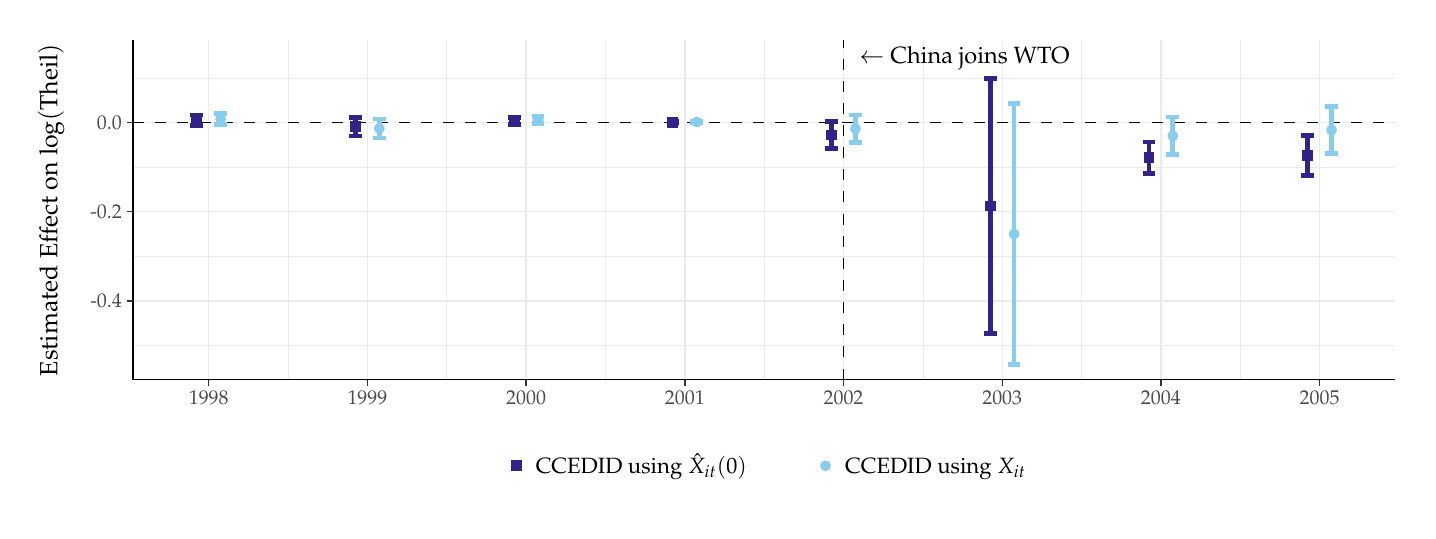
\begin{tikzpicture}[x=1pt,y=1pt]
\definecolor{fillColor}{RGB}{255,255,255}
\path[use as bounding box,fill=fillColor] (0,0) rectangle (498.66,174.53);
\begin{scope}
\path[clip] (  0.00,  0.00) rectangle (498.66,174.53);
\definecolor{drawColor}{RGB}{255,255,255}

\path[draw=drawColor,line width= 0.5pt,line join=round,line cap=round,fill=fillColor] ( -0.00,  0.00) rectangle (498.66,174.53);
\end{scope}
\begin{scope}
\path[clip] ( 38.10, 47.36) rectangle (494.16,170.03);
\definecolor{fillColor}{RGB}{255,255,255}

\path[fill=fillColor] ( 38.10, 47.36) rectangle (494.16,170.03);
\definecolor{drawColor}{gray}{0.92}

\path[draw=drawColor,line width= 0.2pt,line join=round] ( 38.10, 59.72) --
	(494.16, 59.72);

\path[draw=drawColor,line width= 0.2pt,line join=round] ( 38.10, 91.94) --
	(494.16, 91.94);

\path[draw=drawColor,line width= 0.2pt,line join=round] ( 38.10,124.17) --
	(494.16,124.17);

\path[draw=drawColor,line width= 0.2pt,line join=round] ( 38.10,156.40) --
	(494.16,156.40);

\path[draw=drawColor,line width= 0.2pt,line join=round] ( 94.09, 47.36) --
	( 94.09,170.03);

\path[draw=drawColor,line width= 0.2pt,line join=round] (151.44, 47.36) --
	(151.44,170.03);

\path[draw=drawColor,line width= 0.2pt,line join=round] (208.78, 47.36) --
	(208.78,170.03);

\path[draw=drawColor,line width= 0.2pt,line join=round] (266.13, 47.36) --
	(266.13,170.03);

\path[draw=drawColor,line width= 0.2pt,line join=round] (323.47, 47.36) --
	(323.47,170.03);

\path[draw=drawColor,line width= 0.2pt,line join=round] (380.82, 47.36) --
	(380.82,170.03);

\path[draw=drawColor,line width= 0.2pt,line join=round] (438.17, 47.36) --
	(438.17,170.03);

\path[draw=drawColor,line width= 0.5pt,line join=round] ( 38.10, 75.83) --
	(494.16, 75.83);

\path[draw=drawColor,line width= 0.5pt,line join=round] ( 38.10,108.06) --
	(494.16,108.06);

\path[draw=drawColor,line width= 0.5pt,line join=round] ( 38.10,140.29) --
	(494.16,140.29);

\path[draw=drawColor,line width= 0.5pt,line join=round] ( 65.42, 47.36) --
	( 65.42,170.03);

\path[draw=drawColor,line width= 0.5pt,line join=round] (122.77, 47.36) --
	(122.77,170.03);

\path[draw=drawColor,line width= 0.5pt,line join=round] (180.11, 47.36) --
	(180.11,170.03);

\path[draw=drawColor,line width= 0.5pt,line join=round] (237.46, 47.36) --
	(237.46,170.03);

\path[draw=drawColor,line width= 0.5pt,line join=round] (294.80, 47.36) --
	(294.80,170.03);

\path[draw=drawColor,line width= 0.5pt,line join=round] (352.15, 47.36) --
	(352.15,170.03);

\path[draw=drawColor,line width= 0.5pt,line join=round] (409.49, 47.36) --
	(409.49,170.03);

\path[draw=drawColor,line width= 0.5pt,line join=round] (466.84, 47.36) --
	(466.84,170.03);
\definecolor{drawColor}{RGB}{0,0,0}

\path[draw=drawColor,line width= 0.6pt,dash pattern=on 4pt off 4pt ,line join=round] ( 38.10,140.29) -- (494.16,140.29);

\path[draw=drawColor,line width= 0.6pt,dash pattern=on 4pt off 4pt ,line join=round] (294.80, 47.36) -- (294.80,170.03);

\node[text=drawColor,anchor=base west,inner sep=0pt, outer sep=0pt, scale=  0.85] at (300.54,161.52) {$\leftarrow$ China joins WTO};
\definecolor{drawColor}{RGB}{51,34,136}

\path[draw=drawColor,line width= 1.7pt,line join=round] ( 58.83,143.01) --
	( 63.41,143.01);

\path[draw=drawColor,line width= 1.7pt,line join=round] ( 61.12,143.01) --
	( 61.12,139.26);

\path[draw=drawColor,line width= 1.7pt,line join=round] ( 58.83,139.26) --
	( 63.41,139.26);

\path[draw=drawColor,line width= 1.7pt,line join=round] (116.17,142.13) --
	(120.76,142.13);

\path[draw=drawColor,line width= 1.7pt,line join=round] (118.46,142.13) --
	(118.46,135.35);

\path[draw=drawColor,line width= 1.7pt,line join=round] (116.17,135.35) --
	(120.76,135.35);

\path[draw=drawColor,line width= 1.7pt,line join=round] (173.52,142.12) --
	(178.10,142.12);

\path[draw=drawColor,line width= 1.7pt,line join=round] (175.81,142.12) --
	(175.81,139.60);

\path[draw=drawColor,line width= 1.7pt,line join=round] (173.52,139.60) --
	(178.10,139.60);

\path[draw=drawColor,line width= 1.7pt,line join=round] (230.86,140.66) --
	(235.45,140.66);

\path[draw=drawColor,line width= 1.7pt,line join=round] (233.16,140.66) --
	(233.16,140.15);

\path[draw=drawColor,line width= 1.7pt,line join=round] (230.86,140.15) --
	(235.45,140.15);

\path[draw=drawColor,line width= 1.7pt,line join=round] (288.21,140.68) --
	(292.79,140.68);

\path[draw=drawColor,line width= 1.7pt,line join=round] (290.50,140.68) --
	(290.50,130.85);

\path[draw=drawColor,line width= 1.7pt,line join=round] (288.21,130.85) --
	(292.79,130.85);

\path[draw=drawColor,line width= 1.7pt,line join=round] (345.55,156.17) --
	(350.14,156.17);

\path[draw=drawColor,line width= 1.7pt,line join=round] (347.85,156.17) --
	(347.85, 64.02);

\path[draw=drawColor,line width= 1.7pt,line join=round] (345.55, 64.02) --
	(350.14, 64.02);

\path[draw=drawColor,line width= 1.7pt,line join=round] (402.90,133.24) --
	(407.49,133.24);

\path[draw=drawColor,line width= 1.7pt,line join=round] (405.19,133.24) --
	(405.19,121.75);

\path[draw=drawColor,line width= 1.7pt,line join=round] (402.90,121.75) --
	(407.49,121.75);

\path[draw=drawColor,line width= 1.7pt,line join=round] (460.24,135.46) --
	(464.83,135.46);

\path[draw=drawColor,line width= 1.7pt,line join=round] (462.54,135.46) --
	(462.54,120.99);

\path[draw=drawColor,line width= 1.7pt,line join=round] (460.24,120.99) --
	(464.83,120.99);
\definecolor{drawColor}{RGB}{136,204,238}

\path[draw=drawColor,line width= 1.7pt,line join=round] ( 67.43,143.39) --
	( 72.01,143.39);

\path[draw=drawColor,line width= 1.7pt,line join=round] ( 69.72,143.39) --
	( 69.72,139.59);

\path[draw=drawColor,line width= 1.7pt,line join=round] ( 67.43,139.59) --
	( 72.01,139.59);

\path[draw=drawColor,line width= 1.7pt,line join=round] (124.77,141.54) --
	(129.36,141.54);

\path[draw=drawColor,line width= 1.7pt,line join=round] (127.07,141.54) --
	(127.07,134.67);

\path[draw=drawColor,line width= 1.7pt,line join=round] (124.77,134.67) --
	(129.36,134.67);

\path[draw=drawColor,line width= 1.7pt,line join=round] (182.12,142.37) --
	(186.71,142.37);

\path[draw=drawColor,line width= 1.7pt,line join=round] (184.41,142.37) --
	(184.41,139.82);

\path[draw=drawColor,line width= 1.7pt,line join=round] (182.12,139.82) --
	(186.71,139.82);

\path[draw=drawColor,line width= 1.7pt,line join=round] (239.46,140.71) --
	(244.05,140.71);

\path[draw=drawColor,line width= 1.7pt,line join=round] (241.76,140.71) --
	(241.76,140.19);

\path[draw=drawColor,line width= 1.7pt,line join=round] (239.46,140.19) --
	(244.05,140.19);

\path[draw=drawColor,line width= 1.7pt,line join=round] (296.81,142.94) --
	(301.40,142.94);

\path[draw=drawColor,line width= 1.7pt,line join=round] (299.10,142.94) --
	(299.10,133.06);

\path[draw=drawColor,line width= 1.7pt,line join=round] (296.81,133.06) --
	(301.40,133.06);

\path[draw=drawColor,line width= 1.7pt,line join=round] (354.15,147.02) --
	(358.74,147.02);

\path[draw=drawColor,line width= 1.7pt,line join=round] (356.45,147.02) --
	(356.45, 52.94);

\path[draw=drawColor,line width= 1.7pt,line join=round] (354.15, 52.94) --
	(358.74, 52.94);

\path[draw=drawColor,line width= 1.7pt,line join=round] (411.50,142.29) --
	(416.09,142.29);

\path[draw=drawColor,line width= 1.7pt,line join=round] (413.79,142.29) --
	(413.79,128.61);

\path[draw=drawColor,line width= 1.7pt,line join=round] (411.50,128.61) --
	(416.09,128.61);

\path[draw=drawColor,line width= 1.7pt,line join=round] (468.85,145.98) --
	(473.43,145.98);

\path[draw=drawColor,line width= 1.7pt,line join=round] (471.14,145.98) --
	(471.14,129.17);

\path[draw=drawColor,line width= 1.7pt,line join=round] (468.85,129.17) --
	(473.43,129.17);
\definecolor{fillColor}{RGB}{51,34,136}

\path[fill=fillColor] ( 59.16,139.18) --
	( 63.08,139.18) --
	( 63.08,143.10) --
	( 59.16,143.10) --
	cycle;

\path[fill=fillColor] (116.50,136.78) --
	(120.43,136.78) --
	(120.43,140.70) --
	(116.50,140.70) --
	cycle;

\path[fill=fillColor] (173.85,138.90) --
	(177.77,138.90) --
	(177.77,142.82) --
	(173.85,142.82) --
	cycle;

\path[fill=fillColor] (231.19,138.44) --
	(235.12,138.44) --
	(235.12,142.36) --
	(231.19,142.36) --
	cycle;

\path[fill=fillColor] (288.54,133.80) --
	(292.46,133.80) --
	(292.46,137.73) --
	(288.54,137.73) --
	cycle;

\path[fill=fillColor] (345.88,108.13) --
	(349.81,108.13) --
	(349.81,112.06) --
	(345.88,112.06) --
	cycle;

\path[fill=fillColor] (403.23,125.53) --
	(407.15,125.53) --
	(407.15,129.46) --
	(403.23,129.46) --
	cycle;

\path[fill=fillColor] (460.57,126.26) --
	(464.50,126.26) --
	(464.50,130.18) --
	(460.57,130.18) --
	cycle;
\definecolor{fillColor}{RGB}{136,204,238}

\path[fill=fillColor] ( 69.72,141.49) circle (  1.96);

\path[fill=fillColor] (127.07,138.11) circle (  1.96);

\path[fill=fillColor] (184.41,141.09) circle (  1.96);

\path[fill=fillColor] (241.76,140.45) circle (  1.96);

\path[fill=fillColor] (299.10,138.00) circle (  1.96);

\path[fill=fillColor] (356.45, 99.98) circle (  1.96);

\path[fill=fillColor] (413.79,135.45) circle (  1.96);

\path[fill=fillColor] (471.14,137.58) circle (  1.96);
\end{scope}
\begin{scope}
\path[clip] (  0.00,  0.00) rectangle (498.66,174.53);
\definecolor{drawColor}{RGB}{0,0,0}

\path[draw=drawColor,line width= 0.5pt,line join=round] ( 38.10, 47.36) --
	( 38.10,170.03);
\end{scope}
\begin{scope}
\path[clip] (  0.00,  0.00) rectangle (498.66,174.53);
\definecolor{drawColor}{gray}{0.30}

\node[text=drawColor,anchor=base east,inner sep=0pt, outer sep=0pt, scale=  0.72] at ( 34.05, 73.35) {-0.4};

\node[text=drawColor,anchor=base east,inner sep=0pt, outer sep=0pt, scale=  0.72] at ( 34.05,105.58) {-0.2};

\node[text=drawColor,anchor=base east,inner sep=0pt, outer sep=0pt, scale=  0.72] at ( 34.05,137.81) {0.0};
\end{scope}
\begin{scope}
\path[clip] (  0.00,  0.00) rectangle (498.66,174.53);
\definecolor{drawColor}{gray}{0.20}

\path[draw=drawColor,line width= 0.5pt,line join=round] ( 35.85, 75.83) --
	( 38.10, 75.83);

\path[draw=drawColor,line width= 0.5pt,line join=round] ( 35.85,108.06) --
	( 38.10,108.06);

\path[draw=drawColor,line width= 0.5pt,line join=round] ( 35.85,140.29) --
	( 38.10,140.29);
\end{scope}
\begin{scope}
\path[clip] (  0.00,  0.00) rectangle (498.66,174.53);
\definecolor{drawColor}{RGB}{0,0,0}

\path[draw=drawColor,line width= 0.5pt,line join=round] ( 38.10, 47.36) --
	(494.16, 47.36);
\end{scope}
\begin{scope}
\path[clip] (  0.00,  0.00) rectangle (498.66,174.53);
\definecolor{drawColor}{gray}{0.20}

\path[draw=drawColor,line width= 0.5pt,line join=round] ( 65.42, 45.11) --
	( 65.42, 47.36);

\path[draw=drawColor,line width= 0.5pt,line join=round] (122.77, 45.11) --
	(122.77, 47.36);

\path[draw=drawColor,line width= 0.5pt,line join=round] (180.11, 45.11) --
	(180.11, 47.36);

\path[draw=drawColor,line width= 0.5pt,line join=round] (237.46, 45.11) --
	(237.46, 47.36);

\path[draw=drawColor,line width= 0.5pt,line join=round] (294.80, 45.11) --
	(294.80, 47.36);

\path[draw=drawColor,line width= 0.5pt,line join=round] (352.15, 45.11) --
	(352.15, 47.36);

\path[draw=drawColor,line width= 0.5pt,line join=round] (409.49, 45.11) --
	(409.49, 47.36);

\path[draw=drawColor,line width= 0.5pt,line join=round] (466.84, 45.11) --
	(466.84, 47.36);
\end{scope}
\begin{scope}
\path[clip] (  0.00,  0.00) rectangle (498.66,174.53);
\definecolor{drawColor}{gray}{0.30}

\node[text=drawColor,anchor=base,inner sep=0pt, outer sep=0pt, scale=  0.72] at ( 65.42, 38.35) {1998};

\node[text=drawColor,anchor=base,inner sep=0pt, outer sep=0pt, scale=  0.72] at (122.77, 38.35) {1999};

\node[text=drawColor,anchor=base,inner sep=0pt, outer sep=0pt, scale=  0.72] at (180.11, 38.35) {2000};

\node[text=drawColor,anchor=base,inner sep=0pt, outer sep=0pt, scale=  0.72] at (237.46, 38.35) {2001};

\node[text=drawColor,anchor=base,inner sep=0pt, outer sep=0pt, scale=  0.72] at (294.80, 38.35) {2002};

\node[text=drawColor,anchor=base,inner sep=0pt, outer sep=0pt, scale=  0.72] at (352.15, 38.35) {2003};

\node[text=drawColor,anchor=base,inner sep=0pt, outer sep=0pt, scale=  0.72] at (409.49, 38.35) {2004};

\node[text=drawColor,anchor=base,inner sep=0pt, outer sep=0pt, scale=  0.72] at (466.84, 38.35) {2005};
\end{scope}
\begin{scope}
\path[clip] (  0.00,  0.00) rectangle (498.66,174.53);
\definecolor{drawColor}{RGB}{0,0,0}

\node[text=drawColor,rotate= 90.00,anchor=base,inner sep=0pt, outer sep=0pt, scale=  0.90] at ( 10.70,108.70) {Estimated Effect on $\log($Theil$)$};
\end{scope}
\begin{scope}
\path[clip] (  0.00,  0.00) rectangle (498.66,174.53);
\definecolor{fillColor}{RGB}{255,255,255}

\path[fill=fillColor] (154.97,  4.50) rectangle (377.29, 27.95);
\end{scope}
\begin{scope}
\path[clip] (  0.00,  0.00) rectangle (498.66,174.53);
\definecolor{fillColor}{RGB}{255,255,255}

\path[fill=fillColor] (162.31,  9.00) rectangle (190.77, 23.45);
\end{scope}
\begin{scope}
\path[clip] (  0.00,  0.00) rectangle (498.66,174.53);
\definecolor{fillColor}{RGB}{51,34,136}

\path[fill=fillColor] (174.58, 14.26) --
	(178.50, 14.26) --
	(178.50, 18.19) --
	(174.58, 18.19) --
	cycle;
\end{scope}
\begin{scope}
\path[clip] (  0.00,  0.00) rectangle (498.66,174.53);
\definecolor{fillColor}{RGB}{255,255,255}

\path[fill=fillColor] (274.09,  9.00) rectangle (302.54, 23.45);
\end{scope}
\begin{scope}
\path[clip] (  0.00,  0.00) rectangle (498.66,174.53);
\definecolor{fillColor}{RGB}{136,204,238}

\path[fill=fillColor] (288.31, 16.23) circle (  1.96);
\end{scope}
\begin{scope}
\path[clip] (  0.00,  0.00) rectangle (498.66,174.53);
\definecolor{drawColor}{RGB}{0,0,0}

\node[text=drawColor,anchor=base west,inner sep=0pt, outer sep=0pt, scale=  0.80] at (183.61, 13.47) {CCEDID using $\hat{X}_{it}(0)$};
\end{scope}
\begin{scope}
\path[clip] (  0.00,  0.00) rectangle (498.66,174.53);
\definecolor{drawColor}{RGB}{0,0,0}

\node[text=drawColor,anchor=base west,inner sep=0pt, outer sep=0pt, scale=  0.80] at (295.38, 13.47) {CCEDID using $X_{it}$};
\end{scope}
\end{tikzpicture}

    \end{subfigure}
    
    \begin{subfigure}[b]{\textwidth}
        \caption{With 2003 Interpolation}
        % Created by tikzDevice version 0.12.3.1 on 2023-05-05 12:23:06
% !TEX encoding = UTF-8 Unicode
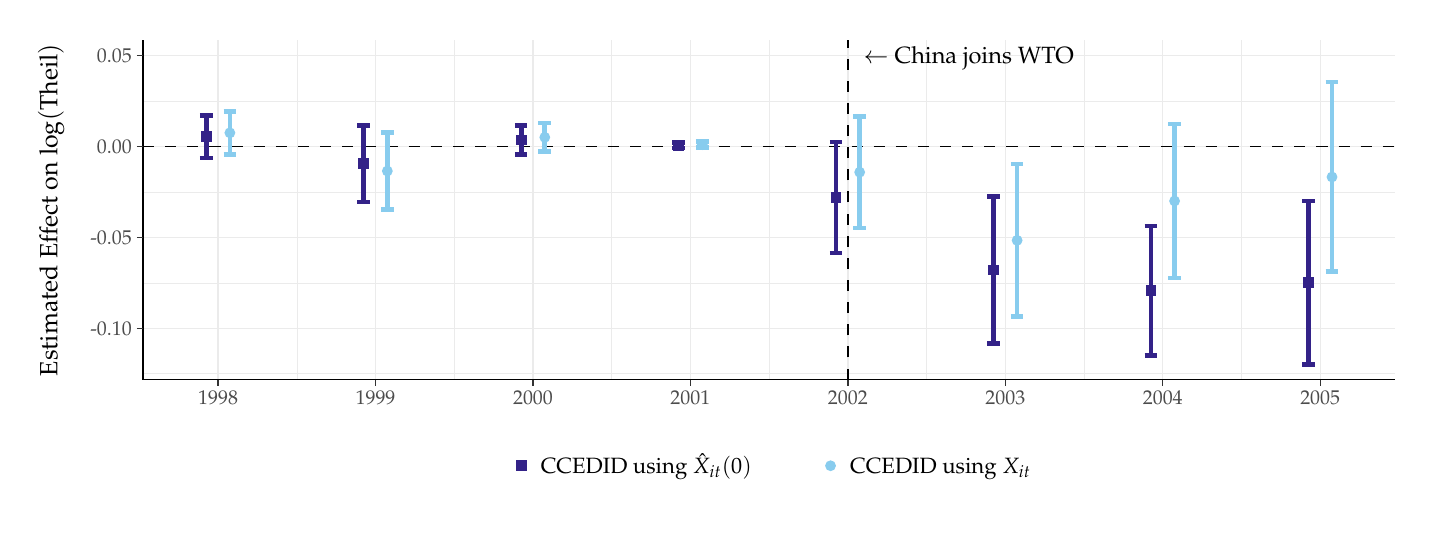
\begin{tikzpicture}[x=1pt,y=1pt]
\definecolor{fillColor}{RGB}{255,255,255}
\path[use as bounding box,fill=fillColor] (0,0) rectangle (498.66,174.53);
\begin{scope}
\path[clip] (  0.00,  0.00) rectangle (498.66,174.53);
\definecolor{drawColor}{RGB}{255,255,255}

\path[draw=drawColor,line width= 0.5pt,line join=round,line cap=round,fill=fillColor] (  0.00,  0.00) rectangle (498.66,174.53);
\end{scope}
\begin{scope}
\path[clip] ( 41.69, 47.36) rectangle (494.16,170.03);
\definecolor{fillColor}{RGB}{255,255,255}

\path[fill=fillColor] ( 41.69, 47.36) rectangle (494.16,170.03);
\definecolor{drawColor}{gray}{0.92}

\path[draw=drawColor,line width= 0.2pt,line join=round] ( 41.69, 49.50) --
	(494.16, 49.50);

\path[draw=drawColor,line width= 0.2pt,line join=round] ( 41.69, 82.34) --
	(494.16, 82.34);

\path[draw=drawColor,line width= 0.2pt,line join=round] ( 41.69,115.19) --
	(494.16,115.19);

\path[draw=drawColor,line width= 0.2pt,line join=round] ( 41.69,148.03) --
	(494.16,148.03);

\path[draw=drawColor,line width= 0.2pt,line join=round] ( 97.25, 47.36) --
	( 97.25,170.03);

\path[draw=drawColor,line width= 0.2pt,line join=round] (154.14, 47.36) --
	(154.14,170.03);

\path[draw=drawColor,line width= 0.2pt,line join=round] (211.04, 47.36) --
	(211.04,170.03);

\path[draw=drawColor,line width= 0.2pt,line join=round] (267.93, 47.36) --
	(267.93,170.03);

\path[draw=drawColor,line width= 0.2pt,line join=round] (324.82, 47.36) --
	(324.82,170.03);

\path[draw=drawColor,line width= 0.2pt,line join=round] (381.71, 47.36) --
	(381.71,170.03);

\path[draw=drawColor,line width= 0.2pt,line join=round] (438.61, 47.36) --
	(438.61,170.03);

\path[draw=drawColor,line width= 0.5pt,line join=round] ( 41.69, 65.92) --
	(494.16, 65.92);

\path[draw=drawColor,line width= 0.5pt,line join=round] ( 41.69, 98.77) --
	(494.16, 98.77);

\path[draw=drawColor,line width= 0.5pt,line join=round] ( 41.69,131.61) --
	(494.16,131.61);

\path[draw=drawColor,line width= 0.5pt,line join=round] ( 41.69,164.46) --
	(494.16,164.46);

\path[draw=drawColor,line width= 0.5pt,line join=round] ( 68.80, 47.36) --
	( 68.80,170.03);

\path[draw=drawColor,line width= 0.5pt,line join=round] (125.70, 47.36) --
	(125.70,170.03);

\path[draw=drawColor,line width= 0.5pt,line join=round] (182.59, 47.36) --
	(182.59,170.03);

\path[draw=drawColor,line width= 0.5pt,line join=round] (239.48, 47.36) --
	(239.48,170.03);

\path[draw=drawColor,line width= 0.5pt,line join=round] (296.38, 47.36) --
	(296.38,170.03);

\path[draw=drawColor,line width= 0.5pt,line join=round] (353.27, 47.36) --
	(353.27,170.03);

\path[draw=drawColor,line width= 0.5pt,line join=round] (410.16, 47.36) --
	(410.16,170.03);

\path[draw=drawColor,line width= 0.5pt,line join=round] (467.05, 47.36) --
	(467.05,170.03);
\definecolor{drawColor}{RGB}{0,0,0}

\path[draw=drawColor,line width= 0.6pt,dash pattern=on 4pt off 4pt ,line join=round] ( 41.69,131.61) -- (494.16,131.61);

\path[draw=drawColor,line width= 0.6pt,dash pattern=on 4pt off 4pt ,line join=round] (296.38, 47.36) -- (296.38,170.03);

\node[text=drawColor,anchor=base west,inner sep=0pt, outer sep=0pt, scale=  0.85] at (302.06,161.52) {$\leftarrow$ China joins WTO};
\definecolor{drawColor}{RGB}{51,34,136}

\path[draw=drawColor,line width= 1.7pt,line join=round] ( 62.26,142.74) --
	( 66.81,142.74);

\path[draw=drawColor,line width= 1.7pt,line join=round] ( 64.54,142.74) --
	( 64.54,127.44);

\path[draw=drawColor,line width= 1.7pt,line join=round] ( 62.26,127.44) --
	( 66.81,127.44);

\path[draw=drawColor,line width= 1.7pt,line join=round] (119.15,139.14) --
	(123.71,139.14);

\path[draw=drawColor,line width= 1.7pt,line join=round] (121.43,139.14) --
	(121.43,111.50);

\path[draw=drawColor,line width= 1.7pt,line join=round] (119.15,111.50) --
	(123.71,111.50);

\path[draw=drawColor,line width= 1.7pt,line join=round] (176.05,139.08) --
	(180.60,139.08);

\path[draw=drawColor,line width= 1.7pt,line join=round] (178.32,139.08) --
	(178.32,128.81);

\path[draw=drawColor,line width= 1.7pt,line join=round] (176.05,128.81) --
	(180.60,128.81);

\path[draw=drawColor,line width= 1.7pt,line join=round] (232.94,133.13) --
	(237.49,133.13);

\path[draw=drawColor,line width= 1.7pt,line join=round] (235.22,133.13) --
	(235.22,131.04);

\path[draw=drawColor,line width= 1.7pt,line join=round] (232.94,131.04) --
	(237.49,131.04);

\path[draw=drawColor,line width= 1.7pt,line join=round] (289.83,133.22) --
	(294.38,133.22);

\path[draw=drawColor,line width= 1.7pt,line join=round] (292.11,133.22) --
	(292.11, 93.13);

\path[draw=drawColor,line width= 1.7pt,line join=round] (289.83, 93.13) --
	(294.38, 93.13);

\path[draw=drawColor,line width= 1.7pt,line join=round] (346.73,113.48) --
	(351.28,113.48);

\path[draw=drawColor,line width= 1.7pt,line join=round] (349.00,113.48) --
	(349.00, 60.44);

\path[draw=drawColor,line width= 1.7pt,line join=round] (346.73, 60.44) --
	(351.28, 60.44);

\path[draw=drawColor,line width= 1.7pt,line join=round] (403.62,102.90) --
	(408.17,102.90);

\path[draw=drawColor,line width= 1.7pt,line join=round] (405.89,102.90) --
	(405.89, 56.04);

\path[draw=drawColor,line width= 1.7pt,line join=round] (403.62, 56.04) --
	(408.17, 56.04);

\path[draw=drawColor,line width= 1.7pt,line join=round] (460.51,111.93) --
	(465.06,111.93);

\path[draw=drawColor,line width= 1.7pt,line join=round] (462.79,111.93) --
	(462.79, 52.94);

\path[draw=drawColor,line width= 1.7pt,line join=round] (460.51, 52.94) --
	(465.06, 52.94);
\definecolor{drawColor}{RGB}{136,204,238}

\path[draw=drawColor,line width= 1.7pt,line join=round] ( 70.79,144.27) --
	( 75.35,144.27);

\path[draw=drawColor,line width= 1.7pt,line join=round] ( 73.07,144.27) --
	( 73.07,128.79);

\path[draw=drawColor,line width= 1.7pt,line join=round] ( 70.79,128.79) --
	( 75.35,128.79);

\path[draw=drawColor,line width= 1.7pt,line join=round] (127.69,136.72) --
	(132.24,136.72);

\path[draw=drawColor,line width= 1.7pt,line join=round] (129.96,136.72) --
	(129.96,108.73);

\path[draw=drawColor,line width= 1.7pt,line join=round] (127.69,108.73) --
	(132.24,108.73);

\path[draw=drawColor,line width= 1.7pt,line join=round] (184.58,140.11) --
	(189.13,140.11);

\path[draw=drawColor,line width= 1.7pt,line join=round] (186.86,140.11) --
	(186.86,129.71);

\path[draw=drawColor,line width= 1.7pt,line join=round] (184.58,129.71) --
	(189.13,129.71);

\path[draw=drawColor,line width= 1.7pt,line join=round] (241.47,133.33) --
	(246.02,133.33);

\path[draw=drawColor,line width= 1.7pt,line join=round] (243.75,133.33) --
	(243.75,131.23);

\path[draw=drawColor,line width= 1.7pt,line join=round] (241.47,131.23) --
	(246.02,131.23);

\path[draw=drawColor,line width= 1.7pt,line join=round] (298.37,142.45) --
	(302.92,142.45);

\path[draw=drawColor,line width= 1.7pt,line join=round] (300.64,142.45) --
	(300.64,102.15);

\path[draw=drawColor,line width= 1.7pt,line join=round] (298.37,102.15) --
	(302.92,102.15);

\path[draw=drawColor,line width= 1.7pt,line join=round] (355.26,125.26) --
	(359.81,125.26);

\path[draw=drawColor,line width= 1.7pt,line join=round] (357.53,125.26) --
	(357.53, 70.10);

\path[draw=drawColor,line width= 1.7pt,line join=round] (355.26, 70.10) --
	(359.81, 70.10);

\path[draw=drawColor,line width= 1.7pt,line join=round] (412.15,139.76) --
	(416.70,139.76);

\path[draw=drawColor,line width= 1.7pt,line join=round] (414.43,139.76) --
	(414.43, 84.03);

\path[draw=drawColor,line width= 1.7pt,line join=round] (412.15, 84.03) --
	(416.70, 84.03);

\path[draw=drawColor,line width= 1.7pt,line join=round] (469.04,154.85) --
	(473.60,154.85);

\path[draw=drawColor,line width= 1.7pt,line join=round] (471.32,154.85) --
	(471.32, 86.30);

\path[draw=drawColor,line width= 1.7pt,line join=round] (469.04, 86.30) --
	(473.60, 86.30);
\definecolor{fillColor}{RGB}{51,34,136}

\path[fill=fillColor] ( 62.57,133.13) --
	( 66.50,133.13) --
	( 66.50,137.05) --
	( 62.57,137.05) --
	cycle;

\path[fill=fillColor] (119.47,123.36) --
	(123.39,123.36) --
	(123.39,127.28) --
	(119.47,127.28) --
	cycle;

\path[fill=fillColor] (176.36,131.98) --
	(180.28,131.98) --
	(180.28,135.91) --
	(176.36,135.91) --
	cycle;

\path[fill=fillColor] (233.25,130.12) --
	(237.18,130.12) --
	(237.18,134.05) --
	(233.25,134.05) --
	cycle;

\path[fill=fillColor] (290.15,111.22) --
	(294.07,111.22) --
	(294.07,115.14) --
	(290.15,115.14) --
	cycle;

\path[fill=fillColor] (347.04, 85.00) --
	(350.96, 85.00) --
	(350.96, 88.92) --
	(347.04, 88.92) --
	cycle;

\path[fill=fillColor] (403.93, 77.51) --
	(407.86, 77.51) --
	(407.86, 81.43) --
	(403.93, 81.43) --
	cycle;

\path[fill=fillColor] (460.82, 80.47) --
	(464.75, 80.47) --
	(464.75, 84.40) --
	(460.82, 84.40) --
	cycle;
\definecolor{fillColor}{RGB}{136,204,238}

\path[fill=fillColor] ( 73.07,136.53) circle (  1.96);

\path[fill=fillColor] (129.96,122.73) circle (  1.96);

\path[fill=fillColor] (186.86,134.91) circle (  1.96);

\path[fill=fillColor] (243.75,132.28) circle (  1.96);

\path[fill=fillColor] (300.64,122.30) circle (  1.96);

\path[fill=fillColor] (357.53, 97.68) circle (  1.96);

\path[fill=fillColor] (414.43,111.90) circle (  1.96);

\path[fill=fillColor] (471.32,120.57) circle (  1.96);
\end{scope}
\begin{scope}
\path[clip] (  0.00,  0.00) rectangle (498.66,174.53);
\definecolor{drawColor}{RGB}{0,0,0}

\path[draw=drawColor,line width= 0.5pt,line join=round] ( 41.69, 47.36) --
	( 41.69,170.03);
\end{scope}
\begin{scope}
\path[clip] (  0.00,  0.00) rectangle (498.66,174.53);
\definecolor{drawColor}{gray}{0.30}

\node[text=drawColor,anchor=base east,inner sep=0pt, outer sep=0pt, scale=  0.72] at ( 37.64, 63.44) {-0.10};

\node[text=drawColor,anchor=base east,inner sep=0pt, outer sep=0pt, scale=  0.72] at ( 37.64, 96.29) {-0.05};

\node[text=drawColor,anchor=base east,inner sep=0pt, outer sep=0pt, scale=  0.72] at ( 37.64,129.13) {0.00};

\node[text=drawColor,anchor=base east,inner sep=0pt, outer sep=0pt, scale=  0.72] at ( 37.64,161.98) {0.05};
\end{scope}
\begin{scope}
\path[clip] (  0.00,  0.00) rectangle (498.66,174.53);
\definecolor{drawColor}{gray}{0.20}

\path[draw=drawColor,line width= 0.5pt,line join=round] ( 39.44, 65.92) --
	( 41.69, 65.92);

\path[draw=drawColor,line width= 0.5pt,line join=round] ( 39.44, 98.77) --
	( 41.69, 98.77);

\path[draw=drawColor,line width= 0.5pt,line join=round] ( 39.44,131.61) --
	( 41.69,131.61);

\path[draw=drawColor,line width= 0.5pt,line join=round] ( 39.44,164.46) --
	( 41.69,164.46);
\end{scope}
\begin{scope}
\path[clip] (  0.00,  0.00) rectangle (498.66,174.53);
\definecolor{drawColor}{RGB}{0,0,0}

\path[draw=drawColor,line width= 0.5pt,line join=round] ( 41.69, 47.36) --
	(494.16, 47.36);
\end{scope}
\begin{scope}
\path[clip] (  0.00,  0.00) rectangle (498.66,174.53);
\definecolor{drawColor}{gray}{0.20}

\path[draw=drawColor,line width= 0.5pt,line join=round] ( 68.80, 45.11) --
	( 68.80, 47.36);

\path[draw=drawColor,line width= 0.5pt,line join=round] (125.70, 45.11) --
	(125.70, 47.36);

\path[draw=drawColor,line width= 0.5pt,line join=round] (182.59, 45.11) --
	(182.59, 47.36);

\path[draw=drawColor,line width= 0.5pt,line join=round] (239.48, 45.11) --
	(239.48, 47.36);

\path[draw=drawColor,line width= 0.5pt,line join=round] (296.38, 45.11) --
	(296.38, 47.36);

\path[draw=drawColor,line width= 0.5pt,line join=round] (353.27, 45.11) --
	(353.27, 47.36);

\path[draw=drawColor,line width= 0.5pt,line join=round] (410.16, 45.11) --
	(410.16, 47.36);

\path[draw=drawColor,line width= 0.5pt,line join=round] (467.05, 45.11) --
	(467.05, 47.36);
\end{scope}
\begin{scope}
\path[clip] (  0.00,  0.00) rectangle (498.66,174.53);
\definecolor{drawColor}{gray}{0.30}

\node[text=drawColor,anchor=base,inner sep=0pt, outer sep=0pt, scale=  0.72] at ( 68.80, 38.35) {1998};

\node[text=drawColor,anchor=base,inner sep=0pt, outer sep=0pt, scale=  0.72] at (125.70, 38.35) {1999};

\node[text=drawColor,anchor=base,inner sep=0pt, outer sep=0pt, scale=  0.72] at (182.59, 38.35) {2000};

\node[text=drawColor,anchor=base,inner sep=0pt, outer sep=0pt, scale=  0.72] at (239.48, 38.35) {2001};

\node[text=drawColor,anchor=base,inner sep=0pt, outer sep=0pt, scale=  0.72] at (296.38, 38.35) {2002};

\node[text=drawColor,anchor=base,inner sep=0pt, outer sep=0pt, scale=  0.72] at (353.27, 38.35) {2003};

\node[text=drawColor,anchor=base,inner sep=0pt, outer sep=0pt, scale=  0.72] at (410.16, 38.35) {2004};

\node[text=drawColor,anchor=base,inner sep=0pt, outer sep=0pt, scale=  0.72] at (467.05, 38.35) {2005};
\end{scope}
\begin{scope}
\path[clip] (  0.00,  0.00) rectangle (498.66,174.53);
\definecolor{drawColor}{RGB}{0,0,0}

\node[text=drawColor,rotate= 90.00,anchor=base,inner sep=0pt, outer sep=0pt, scale=  0.90] at ( 10.70,108.70) {Estimated Effect on $\log($Theil$)$};
\end{scope}
\begin{scope}
\path[clip] (  0.00,  0.00) rectangle (498.66,174.53);
\definecolor{fillColor}{RGB}{255,255,255}

\path[fill=fillColor] (156.77,  4.50) rectangle (379.09, 27.95);
\end{scope}
\begin{scope}
\path[clip] (  0.00,  0.00) rectangle (498.66,174.53);
\definecolor{fillColor}{RGB}{255,255,255}

\path[fill=fillColor] (164.11,  9.00) rectangle (192.57, 23.45);
\end{scope}
\begin{scope}
\path[clip] (  0.00,  0.00) rectangle (498.66,174.53);
\definecolor{fillColor}{RGB}{51,34,136}

\path[fill=fillColor] (176.38, 14.26) --
	(180.30, 14.26) --
	(180.30, 18.19) --
	(176.38, 18.19) --
	cycle;
\end{scope}
\begin{scope}
\path[clip] (  0.00,  0.00) rectangle (498.66,174.53);
\definecolor{fillColor}{RGB}{255,255,255}

\path[fill=fillColor] (275.89,  9.00) rectangle (304.34, 23.45);
\end{scope}
\begin{scope}
\path[clip] (  0.00,  0.00) rectangle (498.66,174.53);
\definecolor{fillColor}{RGB}{136,204,238}

\path[fill=fillColor] (290.11, 16.23) circle (  1.96);
\end{scope}
\begin{scope}
\path[clip] (  0.00,  0.00) rectangle (498.66,174.53);
\definecolor{drawColor}{RGB}{0,0,0}

\node[text=drawColor,anchor=base west,inner sep=0pt, outer sep=0pt, scale=  0.80] at (185.41, 13.47) {CCEDID using $\hat{X}_{it}(0)$};
\end{scope}
\begin{scope}
\path[clip] (  0.00,  0.00) rectangle (498.66,174.53);
\definecolor{drawColor}{RGB}{0,0,0}

\node[text=drawColor,anchor=base west,inner sep=0pt, outer sep=0pt, scale=  0.80] at (297.18, 13.47) {CCEDID using $X_{it}$};
\end{scope}
\end{tikzpicture}

    \end{subfigure}
    
    {\footnotesize\emph{Notes:} These figures presents event-study estimates and 95\% confidence intervals for the effect of China WTO ascension on the dispersion of firm-level markups within an industry defined by the Theil index given in (\ref{eq:theil_index}). Treatment is equal to one for industries with above-median 2001 tariff rates with China for years 2002 and beyond. Estimates are computed using the CCEDID estimator proposed in the paper with the Theil index of firm-level total factor productivity as the covariate X. A constant factor is included as an observed factor. Panel (a) presents estimates of the total effect of WTO Ascension, $\Delta$, and panel (b) presents the portion of the effect mediated by the Theil index in firm-level total factor productivity. This figure replaces the Theil index in firm-level total factor productivity for 2003 with the linear intepolation between 2002 and 2004 as discussed in the text.}
\end{figure}





% ------------------------------------------------------------------------------
\section{Conclusion}
% ------------------------------------------------------------------------------

%12/3/2022 draft. This needs to be cleaned up, but I just wanted to get something down. 


We derive a consistent estimator of ATTs when untreated potential outcomes are generated by an interactive fixed effects error. Our identification strategy, based on the popular common correlated effects model, relies on time- and individual-varying covariates that admit a pure factor structure. We use the cross-sectional averages of the data to impute the untreated potential outcomes in post-treatment time periods. Our main consistency result allows for a fixed number of time periods, but can easily extend to when there are many pre-treatment observations. 

While most treatment effect analyses omit time-varying covariates due to their possible correlation with treatment status, we explicitly allow treatment to affect the covariates' distribution in an arbitrary way. This model allows us to decompose the effect of treatment via a direct effect on the level of the outcomes and a mediated effect through the covariates. Such a decomposition allows researchers to perform inference on the possible mechanisms of an intervention through different relevant channels. We also demonstrate how estimators based on time-varying controls that do not allow indirect effects, such as the principal components estimator of \citet{chan2022pcdid}, are only consistent for the direct effect of treatment unless either the covariates are independent of treatment status or have zero effect on the outcome. This effect is consistently estimated by our CCE estimator under a weaker model proposed by \citet{Brown_Schmidt_Wooldridge_2021}. 

We illustrated the importance of this decomposition in our analysis of markup dispersion. Our estimator is able to quantify potential mechanisms \emph{underlying} an estimated causal effect. In our example, we show that a decrease in marginal cost markups explain 25\% of the estimated decrease in the dispersion of markups among U.S. industries after China entered the WTO. Our results are similar to the existing literature and provide causal evidence on the importance of total factor productivity dispersion on markup dispersion.





% ------------------------------------------------------------------------------
\pagebreak
\bibliography{references}
% ------------------------------------------------------------------------------


\pagebreak

\appendix

%\numberwithin{equation}{section}
\renewcommand{\theequation}{A.\arabic{equation}}\textbf{}

\section*{Appendix}

\noindent \textbf{Proof of Theorem 1.}

\medskip

\noindent We start with part (a). We begin by considering the step-1 estimator of $\*f_t$. In so doing, it is useful to denote by $\overline{\*a}_t = N_{\infty}^{-1}\sum_{i = 1}^N D_{i,\infty} \*a_{i,t}$ the cross-sectional average of any vector $\*a_{i,t}$ for the group of untreated units. In this notation, $\widehat{\*{f}}_t = \overline {\*z}_t$. By inserting \eqref{x} into \eqref{fhat}, and noting that $B_t = 0$ in the pretreatment sample when $t \leq T_0$, we obtain
\begin{equation}\label{fhat1}
\widehat{\*{f}}_t = \overline {\*{z}}_t = \overline{\+\Lambda}'\*{f}_t + \overline {\*e}_{t},
\end{equation}
If $m+1=r$, $\overline{\+\Lambda}$ is full rank and invertible, which means that \eqref{fhat1} can be rewritten as
\begin{equation}\label{redefined}
    \overline{\+\Lambda}^{-1\prime}\widehat{\*{f}}_t=\*{f}_t+\overline{\+\Lambda}^{-1\prime}\overline{\*e}_t .
\end{equation}
Because $\|\overline{\*e}_t\|=O_p(N^{-1/2})$ under Assumption 4, we have
\begin{equation}\label{redefined2}
\overline{\+\Lambda}^{-1\prime}\widehat{\*{f}}_t = \*{f}_t + O_p(N^{-1/2})
\end{equation}
and hence $\overline{\+\Lambda}^{-1\prime} \widehat{\*{f}}_t$ is consistent for $\*{f}_t$. In practice, we never observe $\overline{\+\Lambda}$. However, since $\+{\alpha}_i'\*{f}_t = \+{\alpha}_i' \overline{\+\Lambda}^{-1\prime}\widehat{\*{f}}_t + O_p(N^{-1/2})$, it is enough if we know $\widehat{\*{f}}_t$, because $\overline{\+\Lambda}^{-1}$ is subsumed in the estimation of the coefficient of $\widehat{\*{f}}_t$, which is $\*a_i$ in our notation.

The above analysis is not possible when $m +1> r$ since $\overline{\+{\Lambda}}$ is no longer invertible. However, we still need something similar to (\ref{redefined}), because it determines the object that is being estimated. The way we approach this issue is the same as in \citet{juodis2021robustness}, and others. In particular, we begin by partitioning $\+{\Lambda}_i$ as $\overline{\+{\Lambda}}=[\overline{\+{\Lambda}}_r, \overline{\+{\Lambda}}_{-r}]$, where $\overline{\+{\Lambda}}_{-r}$ is $r\times (m+1-r)$ and $\overline{\+{\Lambda}}_r$ is $r \times r$ and full rank. Note that this partition is without loss of generality under Assumption 6. We then introduce the following $(m+1)\times (m+1)$ rotation matrix, which is chosen such that $\overline{\+{\Lambda}}\overline{\*{H}}= [\*{I}_r, \*{0}_{r\times (m+1-r)}]$ and that is going to play the same role as $\overline{\+{\Lambda}}^{-1}$ under $m+1=r$:
\begin{equation}
    \overline{\*{H}} =\left[\begin{array}{cc}\overline{\+{\Lambda}}_r^{-1} & -\overline{\+{\Lambda}}_r^{-1}\overline{\+{\Lambda}}_{-r}\\
    \*{0}_{(m+1-r)\times r} & \*{I}_{m+1-r}\end{array}\right]=[\overline{\*{H}}_r,\, \overline{\*{H}}_{-r}],
\end{equation}
where $\overline{\*{H}}_r=[\overline{\+{\Lambda}}_r^{-1\prime}, \*{0}_{r\times (m+1-r)} ]'$ is $(m+1)\times r$, while $\overline{\*{H}}_{-r}=[ -\overline{\+{\Lambda}}_{-r}'\overline{\+{\Lambda}}_r^{-1\prime}, \*{I}_{m+1-r}]'$ is $(m+1)\times (m+1-r)$. If $m+1=r$, we define $\overline{\*{H}}=\overline{\*{H}}_r=\overline{\+{\Lambda}}_r^{-1}=\overline{\+{\Lambda}}^{-1}$. We further introduce the $(m+1)\times (m+1)$ matrix $\*{D}_N= \mathrm{diag}(\*{I}_r , \sqrt{N}\*{I}_{m+1-r})$ with $\*{D}_N=\*{I}_{m+1}$ if $m+1=r$. By pre-multiplying $\widehat{\*{f}}_t$ by $\*{D}_N\overline{\*{H}}'$, we obtain
\begin{equation}\label{fhat0}
    \*{D}_N\overline{\*{H}}'\widehat{\*{f}}_t=\widehat{\*{f}}^0_t= \*{D}_N\overline{\*{H}}'\overline{\+{\Lambda}}'\*{f}_t+ \*{D}_N\overline{\*{H}}'\overline{\*e}_t=\*{f}^0_t+\overline{\*e}^0_t,
\end{equation}
where $\*{f}^0_t=[\*{f}'_t, \*{0}_{(m+1-r)\times 1}']'$ and $\overline{\*e}^0_t=[\overline{\*e}_{t}'\overline{\*H}_r, \sqrt{N}\overline{\*{e}}_{t}'\overline{\*H}_{-r}]'=
[\overline{\*{e}}^{0\prime}_{r,t}, \overline{\*{e}}^{0\prime}_{-r,t}]'$ are both $(m+1)\times 1$ with $\overline{\*{e}}_{r,t}^0$ and $\overline{\*{e}}_{-r,t}^0$ being $r\times 1$ and $(m+1-r)\times 1$, respectively. Hence, since $\|\overline{\*{e}}_{r,t}^0\| =O_p(N^{-1/2})$ and $\|\overline{\*{e}}_{-r,t}^0\| =O_p(1)$, when $m + 1> r$ we are no longer estimating $\*{f}_t$ but rather $\*f_t^+ = [\*{f}_t', \overline{\*{e}}_{-r,t}^{0\prime}]'$;
\begin{align}
\widehat{\*{f}}_t^0 = \*f_t^{0} + \overline{\*e}_t^{0} = \left[\begin{array}{c} \*f_t \\
    \*{0}_{(m+1-r)\times 1} \end{array}\right] + \left[\begin{array}{c} \overline{\*e}_{r,t}^{0} \\
    \overline{\*e}_{-r,t}^{0} \end{array}\right] = \*f_t^+ +  O_p(N^{-1/2}),
\end{align}
The fact that $\*{f}_t$ is included in $\*f_t^+$ suggests that asymptotically CCEDID should be able to account for the unknown factors even if $m + 1> r$. By ensuring the existence of $\overline{\*{H}}$, Assumption 6 makes this possible. However, we also note that because of the presence of $\overline{\*{e}}_{-r,t}^0$, the asymptotic distribution theory will in general depend on whether $m+1=r$ or $m +1> r$.

It is useful to be able to use the above notation not only when $m+1> r$ but also when $m+1=r$. We therefore define $\widehat{\*{f}}^0_t=\overline{\+{\Lambda}}^{-1\prime}\widehat{\*{f}}_t$, $\*{f}^0_t = \*{f}_t$ and $\overline{\*{e}}^0_t = \overline{\+{\Lambda}}^{-1\prime}\overline{\*{e}}_t$ if $m+1=r$, so that we are back in (\ref{redefined}).

Let us now consider $\widehat \Delta_{i,g,t}$, which, unlike $\widehat{\*f}_t$, is computed based on treated units in post-treatment periods ($i\in \mathcal{I}_g$, $g < G$ and $t \geq T_g$). From Assumption 3, and the definitions of $y_{i,t}$ and $\widehat y_{i,t}(0)$, 
\begin{align}
\widehat \Delta_{i,g,t} & = y_{i,t} - \widehat y_{i,t}(\infty) \notag\\
& = \eta_{i,g,t} + \+\beta_i'\*x_{i,t} + \+\alpha_i'\*f_t + \varepsilon_{i,t} - [\widehat{\+\beta}'\widehat{\*x}_{i,t}(\infty) + \widehat{\*a}_i'\widehat{\*f}_t]  \notag\\
& = \eta_{i,g,t} + \+\beta_i'\*x_{i,t} + \+\alpha_i'\*f_t + \varepsilon_{i,t} - (\widehat{\+\beta}'\*x_{i,t} + \widehat{\*a}_i'\widehat{\*f}_t) + \widehat{\+\beta}'[\*x_{i,t} - \widehat{\*x}_{i,t}(\infty)]  \notag\\
& = \eta_{i,g,t} - (\widehat{\+\beta} - \+\beta_i)'\*x_{i,t}- (\widehat{\*a}_i'\widehat{\*f}_t - \+\alpha_i'\*f_t)  + \widehat{\+\beta}'[\*x_{i,t} - \widehat{\*x}_{i,t}(\infty)] + \varepsilon_{i,t} \notag\\
& = \eta_{i,g,t} - (\widehat{\+\beta} - \+\beta_i)'\*x_{i,t} - (\widehat{\*a}_i'\widehat{\*f}_t - \+\alpha_i'\*f_t)  + \widehat{\+\beta}'[\*x_{i,t} - \widehat{\*x}_{i,t}(\infty)] + \varepsilon_{i,t} ,
\end{align}
where the last equality makes use of the fact that $D_iB_t = 1$ for all $i\in \mathcal{I}_g$, $g < G$ and $t \geq T_g$. Consider $\widehat{\*a}_i'\widehat{\*f}_t - \+\alpha_i'\*f_t$. While the $(m+1)\times r$ matrix $\mathbf{D}_N\overline{\mathbf{H}}'\overline{\boldsymbol{\Lambda}}'$ is not necessarily square under Assumption 6, it has full column rank. This means that we can compute its Moore--Penrose inverse, which is given by $(\mathbf{D}_N\overline{\mathbf{H}}'\overline{\boldsymbol{\Lambda}}')^+ = (\mathbf{D}_N\overline{\mathbf{H}}'\overline{\boldsymbol{\Lambda}}')' = [ \mathbf{I}_r, \mathbf{0}_{r\times (m+1-r)} ]$, such that $(\mathbf{D}_N\overline{\mathbf{H}}'\overline{\boldsymbol{\Lambda}}')^+ \mathbf{D}_N\overline{\mathbf{H}}'\overline{\boldsymbol{\Lambda}}' = \mathbf{I}_r$. Hence, $\mathbf{D}_N\overline{\mathbf{H}}'\overline{\boldsymbol{\Lambda}}'\*f_t = [\*f_t', \mathbf{0}_{(m+1-r)\times 1}']' = \*f_t^0$ and we also have $\*{D}_N\overline{\*{H}}'\widehat{\*{f}}_t=\widehat{\*{f}}^0_t$. Making use of this, and letting $\widehat{\*a}_i^0 = (\*{D}_N\overline{\*{H}}')^{-1\prime}\widehat{\*a}_i= (\overline{\*{H}}\*{D}_N)^{-1}\widehat{\*a}_i$ and $\+\alpha_i^0 = (\mathbf{D}_N\overline{\mathbf{H}}'\overline{\boldsymbol{\Lambda}}')^{+\prime} \+\alpha_i= \mathbf{D}_N\overline{\mathbf{H}}'\overline{\boldsymbol{\Lambda}}'\+\alpha_i = [ \+\alpha_i ', \mathbf{0}_{1\times (m+1-r)} ]'$,
\begin{align}
\widehat{\*a}_i'\widehat{\*f}_t - \+\alpha_i'\*f_t &= \widehat{\*a}_i'(\*{D}_N\overline{\*{H}}')^{-1}\*{D}_N\overline{\*{H}}'\widehat{\*f}_t - \+\alpha_i'(\mathbf{D}_N\overline{\mathbf{H}}'\overline{\boldsymbol{\Lambda}}')^+\mathbf{D}_N\overline{\mathbf{H}}'\overline{\boldsymbol{\Lambda}}'\*f_t \notag\\
& = \widehat{\*a}_i^{0\prime}\widehat{\*f}_t^0 - \+\alpha_i^{0\prime}\*f_t^0 \notag\\
& = \+\alpha_i^{0\prime}(\widehat{\*f}_t^0-\*f_t^0) + (\widehat{\*a}_i^{0} - \+\alpha_i^0)'\widehat{\*f}_t^0,
\end{align}
from which it follows that
\begin{align}
\widehat \Delta_{i,g,t}  = \eta_{i,g,t} - (\widehat{\+\beta} - \+\beta_i)'\*x_{i,t}  - \+\alpha_i^{0\prime}(\widehat{\*f}_t^0-\*f_t^0) - (\widehat{\*a}_i^{0} - \+\alpha_i^0)'\widehat{\*f}_t^0  + \widehat{\+\beta}'[\*x_{i,t} - \widehat{\*x}_{i,t}(0)] + \varepsilon_{i,t}
\end{align}

Amongst the terms appearing on the right-hand side of the above equation, the one involving $\widehat{\*a}_i^0 - \+\alpha_i^0$ requires most work. We therefore start with this. Note first that since $\widehat{\*a}_i$ is estimated based on the pretreatment period only, $D_i = 0$. By using this and $\overline{\+\Lambda}\overline{\*H}_{r} = \*I_{r}$, we get
\begin{eqnarray}
\*y_{i}= \*x_{i}\+\beta_i + \widehat{\*f}\overline{\*H}_{r}\+\alpha_i - (\widehat{\*f} - \*f\overline{\+\Lambda})\overline{\*H}_{r}\+\alpha_i+  \+\varepsilon_{i}  = \*x_{i}\+\beta_i + \widehat{\*f} \overline{\*H}_{r}\+\alpha_i - \overline{\*e}_{r}^0\+\alpha_i +  \+\varepsilon_{i}, \label{ystack}
\end{eqnarray}
where the $T_0$-rowed matrices $\*f$ and $\+\varepsilon_{i}$ are defined analogously to $\*y_{i}$, $\*x_{i}$ and $\widehat{\*f}$. Note also that in the notation of the step-2 regression in \eqref{preregr}, we have $\*a_i = \overline{\*H}_{r}\+\alpha_i$. By inserting this and \eqref{ystack} into the expression given for $\widehat{\*a}_i$ in step 2,
\begin{align}
\widehat{\*a}_i &= (\widehat{\*f}'\widehat{\*f})^{-1}\widehat{\*f}'(\*y_{i}-\*x_{i}\widehat{\+\beta}) \notag\\
& = (\widehat{\*f}'\widehat{\*f})^{-1}\widehat{\*f}'(\*x_{i}\+\beta_i + \widehat{\*f} \*a_i - \overline{\*e}_{r}^0\+\alpha_i +  \+\varepsilon_{i}-\*x_{i}\widehat{\+\beta}) \notag\\
& =  \*a_i + (\widehat{\*f}'\widehat{\*f})^{-1}\widehat{\*f}'[- \*x_{i}(\widehat{\+\beta}-\+\beta_i)  - \overline{\*e}_{r}^0\+\alpha_i +  \+\varepsilon_{i} ],
\end{align}
implying
\begin{align}
\widehat{\*a}_i^0 & = (\overline{\*{H}}\*{D}_N)^{-1}\widehat{\*a}_i \notag\\
& = (\overline{\*{H}}\*{D}_N)^{-1}\*a_i + (\overline{\*{H}}\*{D}_N)^{-1}(\widehat{\*f}'\widehat{\*f})^{-1}\widehat{\*f}'[- \*x_{i}(\widehat{\+\beta}-\+\beta_i) - \overline{\*e}_{r}^0\+\alpha_i +  \+\varepsilon_{i} ] \notag\\
& = (\overline{\*{H}}\*{D}_N)^{-1}\*a_i +  (
\*{D}_N\overline{\*{H}}'\widehat{\*f}'\widehat{\*f}\overline{\*{H}}\*{D}_N)^{-1}\*{D}_N\overline{\*{H}}'\widehat{\*f}' [ - \*x_{i}(\widehat{\+\beta}-\+\beta_i)  - \overline{\*e}_{r}^0\+\alpha_i +  \+\varepsilon_{i}]
\notag\\
& = (\overline{\*{H}}\*{D}_N)^{-1}\*a_i + (\widehat{\*f}^{0\prime}\widehat{\*f}^0)^{-1}\widehat{\*f}^{0\prime}[- \*x_{i}(\widehat{\+\beta}-\+\beta_i)  - \overline{\*e}_{r}^0\+\alpha_i +  \+\varepsilon_{i} ]
\end{align}
where $\widehat{\*f}^0 = [\widehat{\*f}_1^0,...,\widehat{\*f}_{T_0}^0]' = \widehat{\*f}\overline{\*{H}}\*{D}_N$ is $T_0\times (m+1)$. Consider the first term on the right-hand side. A direct calculation using the rules for the inverse of a partitioned matrix (see, for example, \citet{abadir2005matrix}, Exercise 5.16) reveals that
\begin{equation}
    (\*{D}_N\overline{\*{H}})^{-1} =\left[\begin{array}{cc}\overline{\+{\Lambda}}_r & \overline{\+{\Lambda}}_{-r}\\
    \*{0}_{(m+1-r)\times r} & N^{-1/2}\*{I}_{m+1-r}\end{array}\right],
\end{equation}
so that
\begin{align}
(\overline{\*{H}}\*{D}_N)^{-1}\overline{\*H}_{r} = \left[\begin{array}{cc}\overline{\+{\Lambda}}_r & \overline{\+{\Lambda}}_{-r}\\
    \*{0}_{(m+1-r)\times r} & N^{-1/2}\*{I}_{m+1-r}\end{array}\right]\left[\begin{array}{c}\overline{\+{\Lambda}}_r^{-1} \\
    \*{0}_{(m+1-r)\times r} \end{array}\right] = \left[\begin{array}{c} \*I_r \\
    \*{0}_{(m+1-r)\times r} \end{array}\right].
\end{align}
This implies
\begin{align}
(\overline{\*{H}}\*{D}_N)^{-1}\*a_i = \left[\begin{array}{c} \+\alpha_i \\
    \*{0}_{(m+1-r)\times 1} \end{array}\right] = \+\alpha_i^0,
\end{align}
leading to the following expression for $\widehat{\*a}_i^0-\+\alpha_i^0$:
\begin{align}
\widehat{\*a}_i^0 - \+\alpha_i^0 & = (\widehat{\*f}^{0\prime}\widehat{\*f}^0)^{-1}\widehat{\*f}^{0\prime}[- \*x_{i}(\widehat{\+\beta}-\+\beta_i)  - \overline{\*e}_{r}^0\+\alpha_i +  \+\varepsilon_{i} ].
\end{align}
We similarly have
\begin{equation}
\widehat{\*x}_{i,t}(\infty) = \widehat{\+\lambda}_i'\widehat{\*f}_t = \*x_i'\widehat{\*f}( \widehat{\*f}' \widehat{\*f} )^{-1} \widehat{\*f}_t= \*x_i'\widehat{\*f}^0( \widehat{\*f}^{0\prime} \widehat{\*f}^0 )^{-1} \widehat{\*f}_t^0 ,
\end{equation}
from which it follows that
\begin{equation}
\widehat{\+\beta}'[\*x_{i,t} - \widehat{\*x}_{i,t}(\infty)] = \widehat{\+\beta}'[\*x_{i,t} - \*x_i'\widehat{\*f}^0( \widehat{\*f}^{0\prime} \widehat{\*f}^0 )^{-1} \widehat{\*f}_t^0].
\end{equation}
By inserting the above expressions into the one given earlier for $\widehat \Delta_{i,g,t}$, we get
\begin{align}
\widehat \Delta_{i,g,t} & = \eta_{i,g,t} - (\widehat{\+\beta} - \+\beta_i)'\*x_{i,t} - \+\alpha_i^{0\prime}(\widehat{\*f}_t^0-\*f_t^0) - (\widehat{\*a}_i^{0} - \+\alpha_i^0)'\widehat{\*f}_t^0 + \widehat{\+\beta}'[\*x_{i,t} - \widehat{\*x}_{i,t}(\infty)] + \varepsilon_{i,t}\notag\\
& = \eta_{i,g,t} - (\widehat{\+\beta} - \+\beta_i)'\*x_{i,t} - \+\alpha_i'\overline{\*e}_{r,t}^0 \notag\\
& - [- \*x_{i}(\widehat{\+\beta}-\+\beta_i)  - \overline{\*e}_{r}^0\+\alpha_i +  \+\varepsilon_{i} ]' \widehat{\*f}^{0} (\widehat{\*f}^{0\prime}\widehat{\*f}^0)^{-1}\widehat{\*f}_t^0 + \widehat{\+\beta}'[\*x_{i,t} - \*x_i'\widehat{\*f}^0( \widehat{\*f}^{0\prime} \widehat{\*f}^0 )^{-1} \widehat{\*f}_t^0] + \varepsilon_{i,t}\notag\\
& = \eta_{i,g,t} + \+\beta_i'\*x_{i,t} - \+\alpha_i'\overline{\*e}_{r,t}^0 + \varepsilon_{i,t} - ( \*x_{i}\+\beta_i  - \overline{\*e}_{r}^0\+\alpha_i +  \+\varepsilon_{i} )' \widehat{\*f}^{0} (\widehat{\*f}^{0\prime}\widehat{\*f}^0)^{-1}\widehat{\*f}_t^0  .
\end{align}
Further use of $\widehat{\*f} = \widehat{\*f}^0\*D_{N}^{-1}\overline{\*H}^{-1}$ gives
\begin{eqnarray}
\*x_i = \*f\+\lambda_i + \*v_i = \widehat{\*f}\overline{\*H}_{r}\+\lambda_i -  (\widehat{\*f} - \*f\overline{\+\Lambda})\overline{\*H}_{r}\+\lambda_i  + \*v_i =  \widehat{\*f}^0\*D_{N}^{-1}\overline{\*H}^{-1}\overline{\*H}_{r}\+\lambda_i  - \overline{\*e}_{r}^0\+\lambda_i  + \*v_i ,
\end{eqnarray}
for $t\leq T_0$. If, on the other hand, $t > T_0$, then 
\begin{eqnarray}
\*x_{i,t} = \+\tau_{i,g,t} + \+\lambda_i'\*f_t + \*v_{i,t} =  \+\tau_{i,g,t} + \+\lambda_i' \overline{\*H}_{r}'\overline{\*H}^{-1\prime}\*D_{N}^{-1}\widehat{\*f}_t^0  - \+\lambda_i'\overline{\*e}_{r,t}^0  + \*v_{i,t}.
\end{eqnarray}
These two last results imply
\begin{align}
& \*x_{i,t} -  \*x_{i}' \widehat{\*f}^{0}(\widehat{\*f}^{0\prime}\widehat{\*f}^0)^{-1}\widehat{\*f}_t^0 \notag\\
& = \+\tau_{i,g,t} + \+\lambda_i' \overline{\*H}_{r}'\overline{\*H}^{-1\prime}\*D_{N}^{-1}\widehat{\*f}_t^0  - \+\lambda_i'\overline{\*e}_{r,t}^0  + \*v_{i,t} -  (\widehat{\*f}^0\*D_{N}^{-1}\overline{\*H}^{-1}\overline{\*H}_{r}\+\lambda_i  - \overline{\*e}_{r}^0\+\lambda_i  + \*v_i)' \widehat{\*f}^{0}(\widehat{\*f}^{0\prime}\widehat{\*f}^0)^{-1}\widehat{\*f}_t^0\notag\\
& = \+\tau_{i,g,t}  - \+\lambda_i'\overline{\*e}_{r,t}^0  + \*v_{i,t} -  ( - \overline{\*e}_{r}^0\+\lambda_i  + \*v_i)' \widehat{\*f}^{0}(\widehat{\*f}^{0\prime}\widehat{\*f}^0)^{-1}\widehat{\*f}_t^0,
\end{align}
and so we arrive at the following expression for $\widehat \Delta_{i,g,t}$:
\begin{align}
\widehat \Delta_{i,g,t} & = \eta_{i,g,t} + \+\beta_i'(\+\tau_{i,g,t}  - \+\lambda_i'\overline{\*e}_{r,t}^0  + \*v_{i,t}) - \+\alpha_i'\overline{\*e}_{r,t}^0 + \varepsilon_{i,t}\notag\\
& - [ (- \overline{\*e}_{r}^0\+\lambda_i  + \*v_i)\+\beta_i  - \overline{\*e}_{r}^0\+\alpha_i +  \+\varepsilon_{i} ]' \widehat{\*f}^{0} (\widehat{\*f}^{0\prime}\widehat{\*f}^0)^{-1}\widehat{\*f}_t^0 \notag\\
& = \Delta_{i,g,t} - (\+\lambda_i\+\beta_i + \+\alpha_i)'\overline{\*e}_{r,t}^0 + \+\beta_i'\*v_{i,t} + \varepsilon_{i,t} \notag\\
& - [ - \overline{\*e}_{r}^0(\+\lambda_i\+\beta_i +\+\alpha_i) + \*v_i\+\beta_i+  \+\varepsilon_{i} ]' \widehat{\*f}^{0} (\widehat{\*f}^{0\prime}\widehat{\*f}^0)^{-1}\widehat{\*f}_t^0  .
\end{align}
where $\Delta_{i,g,t} = \eta_{i,g,t} + \+\beta_i'\+\tau_{i,g,t}$ as defined at the end of Section 2.

The above expression for $\widehat \Delta_{i,g,t}$ is the cleanest possible without exploiting the fact that $N$ is large. Hence, in what remains we are going to let $N\to\infty$. We begin by considering $\widehat{\*f}^{0} (\widehat{\*f}^{0\prime}\widehat{\*f}^0)^{-1}\widehat{\*f}_t^0$. Define $\*f^+ = [\*f_1^+,... \*f_{T_0}^+]' = [\*f, \overline{\*e}_{-r}^{0}]$, a $T_0\times (m+1)$ matrix. We have already shown that $\widehat{\*{f}}^0 = \*f^+ +  O_p(N^{-1/2})$. By using this and the results provided in the proof of Lemma A.1 in \citet{westerlund2019cce}, we have that $\|\widehat{\*f}^{0\prime}\widehat{\*f}^0 - \*f^{+\prime}\*f^+\|= O_p(N^{-1/2})$ and, more importantly,
\begin{align}
\|(\widehat{\*f}^{0\prime}\widehat{\*f}^0 )^{-1} - (\*f^{+\prime}\*f^+)^{-1}\| = O_p(N^{-1/2}),
\end{align}
where
\begin{align}
\*f^{+\prime}\*f^+ &= \left[\begin{array}{cc} \*f'\*f & \*f'\overline{\*e}_{-r}^0 \\ \overline{\*e}_{-r}^{0\prime}\*f  & \overline{\*e}_{-r}^{0\prime}\overline{\*e}_{-r}^0 \end{array}\right] ,\\
(\*f^{+\prime}\*f^+)^{-1} &= \left[\begin{array}{c} (\*f'\*f)^{-1} + (\*f'\*f)^{-1}\*f'\overline{\*e}_{-r}^0(\overline{\*e}_{-r}^{0\prime}\*M_{\*f}\overline{\*e}_{-r}^0)^{-1}\overline{\*e}_{-r}^{0\prime} \*f(\*f'\*f)^{-1}  \\
-(\overline{\*e}_{-r}^{0\prime}\*M_{\*f}\overline{\*e}_{-r}^0)^{-1}\overline{\*e}_{-r}^{0\prime}\*f (\*f'\*f)^{-1} \end{array}\right. \notag\\
& \left. \begin{array}{c}  -(\*f'\*f)^{-1}\*f'\overline{\*e}_{-r}^0(\overline{\*e}_{-r}^{0\prime}\*M_{\*f}\overline{\*e}_{-r}^0)^{-1} \\
 (\overline{\*e}_{-r}^{0\prime}\*M_{\*f}\overline{\*e}_{-r}^0)^{-1} \end{array}\right].
\end{align}
The expression for $(\*f^{+\prime}\*f^+)^{-1}$ is again obtained by using the rules for the inverse of a partitioned matrix. The fact that $\|(\widehat{\*f}^{0\prime}\widehat{\*f}^0 )^{-1} - (\*f^{+\prime}\*f^+)^{-1}\| = O_p(N^{-1/2})$ together with $\widehat{\*{f}}^0 = \*f^+ +  O_p(N^{-1/2})$ imply that
\begin{align}
\widehat{\*f}_t^{0\prime}(\widehat{\*f}^{0\prime}\widehat{\*f}^0)^{-1}\widehat{\*f}^{0\prime} & =  \widehat{\*f}_t^{0\prime}[(\widehat{\*f}^{0\prime}\widehat{\*f}^0)^{-1} - (\*f^{+\prime}\*f^+)^{-1} ]\widehat{\*f}^{0\prime} + \widehat{\*f}_t^{0\prime}(\*f^{+\prime}\*f^+)^{-1}\widehat{\*f}^{0\prime} \notag\\
& = \widehat{\*f}_t^{0\prime}(\*f^{+\prime}\*f^+)^{-1}\widehat{\*f}^{0\prime} + O_p(N^{-1/2})\notag\\
& = \*f_t^{+\prime}(\*f^{+\prime}\*f^+)^{-1}\*f^{+\prime} + O_p(N^{-1/2}).
\end{align}
where, defining $\*M_{\*f}$ analogously to $\*M_{\widehat{\*f}}$,
\begin{align}
& \*f_t^{+\prime}(\*f^{+\prime}\*f^+)^{-1}\*f^{+\prime} \notag\\
& = [\*f_t', \overline{\*e}_{-r,t}^{0\prime}]\left[\begin{array}{c} (\*f'\*f)^{-1} + (\*f'\*f)^{-1}\*f'\overline{\*e}_{-r}^0(\overline{\*e}_{-r}^{0\prime}\*M_{\*f}\overline{\*e}_{-r}^0)^{-1}\overline{\*e}_{-r}^{0\prime} \*f(\*f'\*f)^{-1}  \\
-(\overline{\*e}_{-r}^{0\prime}\*M_{\*f}\overline{\*e}_{-r}^0)^{-1}\overline{\*e}_{-r}^{0\prime}\*f (\*f'\*f)^{-1} \end{array}\right. \notag\\
& \left. \begin{array}{c}  -(\*f'\*f)^{-1}\*f'\overline{\*e}_{-r}^0(\overline{\*e}_{-r}^{0\prime}\*M_{\*f}\overline{\*e}_{-r}^0)^{-1} \\
 (\overline{\*e}_{-r}^{0\prime}\*M_{\*f}\overline{\*e}_{-r}^0)^{-1} \end{array}\right]\left[\begin{array}{c} \*f' \\
    \overline{\*e}_{-r}^{0\prime} \end{array}\right]  \notag\\
& = \*f_t'(\*f'\*f)^{-1}\*f'[\*I_{T_0} -  \overline{\*e}_{-r}^{0}(\overline{\*e}_{-r}^{0\prime}\*M_{\*f}\overline{\*e}_{-r}^0)^{-1} \overline{\*e}_{-r}^{0\prime}\*M_{\*f}] + \overline{\*e}_{-r,t}^{0\prime}(\overline{\*e}_{-r}^{0\prime}\*M_{\*f}\overline{\*e}_{-r}^0)^{-1}\overline{\*e}_{-r}^{0\prime}\*M_{\*f}.
\end{align}
The fact that $\|\widehat{\*f}_t^{0\prime}(\widehat{\*f}^{0\prime}\widehat{\*f}^0)^{-1}\widehat{\*f}^{0\prime} - \*f_t^{+\prime}(\*f^{+\prime}\*f^+)^{-1}\*f^{+\prime}\| = O_p(N^{-1/2})$ implies
\begin{align}
\widehat \Delta_{i,g,t} & = \Delta_{i,g,t} - (\+\lambda_i\+\beta_i + \+\alpha_i)'\overline{\*e}_{r,t}^0 + \+\beta_i'\*v_{i,t} + \varepsilon_{i,t} \notag\\
& - [ - \overline{\*e}_{r}^0(\+\lambda_i\+\beta_i +\+\alpha_i) + \*v_i\+\beta_i+  \+\varepsilon_{i} ]'  \*f^{+} (\*f^{+\prime}\*f^+)^{-1}\*f_t^+ + O_p(N^{-1/2})\notag\\
& = \Delta_{i,g,t} - (\+\lambda_i\+\beta_i + \+\alpha_i)'\overline{\*e}_{r,t}^{0\ast} + \+\beta_i'\*v_{i,t}^* + \varepsilon_{i,t}^*  + O_p(N^{-1/2}),
\end{align}
where
\begin{align}
\*a_{i,t}^* = \*a_{i,t} - \*a_i' \*f^{+} (\*f^{+\prime}\*f^+)^{-1}\*f_t^+ = \*a_{i,t} - \sum_{s=1}^{T_0} \*a_{i,s}\*f_s^{+\prime} (\*f^{+\prime}\*f^+)^{-1}\*f_t^+
\end{align}
for any vector $\*a_{i,t}$ with $T_0$-rowed stack $\*a_i = [\*a_{i,1},...,\*a_{i,T_0}]'$. In words, $\*a_{i,t}^*$ is the limiting ``defactored'' version of $\*a_{i,t}$.

We now make use of the above expression for $\widehat \Delta_{i,g,t}$ to evaluate $\widehat \Delta_{g,t}$. In so doing, it is important to note that the order of the reminder incurred when replacing $\widehat{\*f}_t^{0\prime}(\widehat{\*f}^{0\prime}\widehat{\*f}^0)^{-1}\widehat{\*f}^{0\prime}$ with $\*f_t^{+\prime}(\*f^{+\prime}\*f^+)^{-1}\*f^{+\prime}$ is the same even after averaging over group $g$ and multiplying by $\sqrt{N_g}$. In order to appreciate this, we make use of the fact that $\|\sqrt{N_g}\overline{\*e}_{r}^0\| = O_p(1)$, and since $\*v_{i}$ and $\+\beta_i$ are independent with $\*v_i$ mean zero and independent also across $i$, we also have $\|N_g^{-1/2}\sum_{i= 1}^{N} D_{i,g} \*v_{i}\+\beta_i\| = O_p(1)$. It follows that
\begin{align}
& \left\|\frac{1}{\sqrt{N_g}}\sum_{i= 1}^{N} D_{i,g}[ - \overline{\*e}_{r}^0(\+\lambda_i\+\beta_i +\+\alpha_i) + \*v_i\+\beta_i+  \+\varepsilon_{i} ] \right\|\notag\\
& \leq \|\sqrt{N_g}\overline{\*e}_{r}^0\|\left\|\frac{1}{N_g} \sum_{i= 1}^{N} D_{i,g} (\+\lambda_i\+\beta_i +\+\alpha_i)\right\| + \left\| \frac{1}{\sqrt{N_g}} \sum_{i= 1}^{N} D_{i,g} \*v_{i}\+\beta_i \right\| +  \left\|\frac{1}{\sqrt{N_g}} \sum_{i= 1}^{N} D_{i,g} \+\varepsilon_{i}\right\| =O_p(1).
\end{align}
We can therefore show that
\begin{align}
& \left\|\frac{1}{\sqrt{N_g}}\sum_{i= 1}^{N} D_{i,g}[ - \overline{\*e}_{r}^0(\+\lambda_i\+\beta_i +\+\alpha_i) + \*v_i\+\beta_i+  \+\varepsilon_{i} ]'[\*f^{+} (\*f^{+\prime}\*f^+)^{-1}\*f_t^+ - \widehat{\*f}^{0} (\widehat{\*f}^{0\prime}\widehat{\*f}^0)^{-1}\widehat{\*f}_t^0] \right\| \notag\\
& \leq
\left\| \frac{1}{\sqrt{N_g}}\sum_{i= 1}^{N} D_{i,g}[ - \overline{\*e}_{r}^0(\+\lambda_i\+\beta_i +\+\alpha_i) + \*v_i\+\beta_i+  \+\varepsilon_{i} ]\right\| \|\*f^{+} (\*f^{+\prime}\*f^+)^{-1}\*f_t^+ - \widehat{\*f}^{0} (\widehat{\*f}^{0\prime}\widehat{\*f}^0)^{-1}\widehat{\*f}_t^0\|\notag\\
& = O_p(N^{-1/2}),
\end{align}
which means that the reminder incurred when replacing $\widehat{\*f}_t^{0\prime}(\widehat{\*f}^{0\prime}\widehat{\*f}^0)^{-1}\widehat{\*f}^{0\prime}$ with $\*f_t^{+\prime}(\*f^{+\prime}\*f^+)^{-1}\*f^{+\prime}$ is $O_p(N^{-1/2})$ after averaging over group $g$ and multiplying by $\sqrt{N_g}$. 

For $\Delta_{i,g,t}$, we make use of the fact that $\Delta_{i,g,t}= \Delta_{g,t} + \upsilon_{i,t}$ and $\+\tau_{i,g,t} = \+\tau_{g,t} + \+\zeta_{i,t}$ for $i\in \mathcal{I}_g$ by Assumption 3, giving
\begin{align}
\Delta_{i,g,t} & = \eta_{i,g,t} + \+\beta_i'\+\tau_{i,g,t} = \Delta_{g,t} + \upsilon_{i,t} + (\+\beta + \+\nu_i)'(\+\tau_{g,t} + \+\zeta_{i,t}) \notag\\
& = \Delta_{g,t}  + \+\beta'\+\tau_{g,t} + \upsilon_{i,t}  + \+\beta'\+\zeta_{i,t} + \+\nu_i'(\+\tau_{g,t} + \+\zeta_{i,t})\notag\\
& = \Delta_{g,t}^0 + \upsilon_{i,t}^0,
\end{align}
where $\Delta_{g,t}^0 = \Delta_{g,t} + \+\beta'\+\nu_{i,t}$ and $\upsilon_{i,t}^0 = \upsilon_{i,t}  + \+\beta'\+\zeta_{i,t} + \+\nu_i'\+\tau_{i,g,t}$.

By putting everything together, 
\begin{align}
 \sqrt{N_g}(\widehat \Delta_{g,t} - \Delta_{g,t}^0) & = \frac{1}{\sqrt{N_g}} \sum_{i= 1}^{N} D_{i,g} (\widehat \Delta_{i,g,t} - \Delta_{g,t}^0) \notag\\
& = \frac{1}{\sqrt{N_g}} \sum_{i= 1}^{N} D_{i,g} (\widehat \Delta_{i,g,t} - \Delta_{i,g,t}^0 + \upsilon_{i,t}^0) \notag\\
& = \frac{1}{\sqrt{N_g}} \sum_{i= 1}^{N} D_{i,g} [\upsilon_{i,t}^0 - (\+\lambda_i\+\beta_i + \+\alpha_i)'\overline{\*e}_{r,t}^{0\ast} + \+\beta_i'\*v_{i,t}^* + \varepsilon_{i,t}^* ] + O_p(N^{-1/2}) .
\end{align}
Moreover, Assumption 2 gives us $N_g/N \to_p \mathds{P}(D_{i,g} = 1)$. Hence, if we also define $\*a_g = \lim_{N\to\infty} N_g^{-1} \sum_{i= 1}^{N} D_{i,g} (\+\lambda_i\+\beta_i + \+\alpha_i)$, the above expression for $\sqrt{N_g}(\widehat \Delta_{g,t} - \Delta_{g,t}^0)$ becomes
\begin{align}
& \sqrt{N_g}(\widehat \Delta_{g,t} - \Delta_{g,t}) \notag\\
&= \frac{1}{\sqrt{N_g}}\sum_{i= 1}^{N} D_{i,g}(\upsilon_{i,t}^0  + \+\beta_i'\*v_{i,t}^* + \varepsilon_{i,t}^*) - \sqrt{\frac{N_g}{N}} \frac{1}{N_g}\sum_{i= 1}^{N} D_{i,g} (\+\lambda_i\+\beta_i + \+\alpha_i)'\sqrt{N}\overline{\*e}_{r,t}^{0\ast} + O_p(N^{-1/2}) \notag\\
&= \frac{1}{\sqrt{N_g}}\sum_{i= 1}^{N} D_{i,g} (\upsilon_{i,t}^0  + \+\beta_i'\*v_{i,t}^* + \varepsilon_{i,t}^* ) - \sqrt{\mathds{P}(D_{i,g} = 1)}\*a_g'\sqrt{N}\overline{\*e}_{r,t}^{0*} + o_p(1).
\end{align}
All the terms on the right-hand side of the above equation are mean zero and independent across $i$ (conditionally on $\*f$). They are therefore asymptotically normal by a central limit law for independent variables. However, they are not uncorrelated with each other, which complicates the calculation of the asymptotic variance. Let us therefore define $\omega_{g,t}^2 = \mathrm{var}(\sqrt{N_g}(\widehat \Delta_{g,t} - \Delta_{g,t})  |\mathcal{C})$, where $\mathcal{C}$ is the sigma-field generated by $\*f$. The asymptotic distribution of $\sqrt{N_g}(\widehat \Delta_{g,t} - \Delta_{g,t})$ as $N\to\infty$ can now be stated in the following way:
\begin{align}
\sqrt{N_g}(\widehat \Delta_{g,t} - \Delta_{g,t}) \to_d MN(0, \omega_{g,t}^2 ),
\end{align}
where $MN(\cdot,\cdot)$ signifies a mixed normal distribution that is normal conditionally on $\mathcal{C}$. This means that the conditional distribution of $\sqrt{N_g}(\widehat \Delta_{g,t} - \Delta_{g,t})/\omega_{g,t}$ is also the unconditional distribution. Hence,
\begin{align}
\frac{\sqrt{N_g}(\widehat \Delta_{g,t} - \Delta_{g,t})}{\omega_{g,t}} \to_d N(0, 1),
\end{align}
as required for part (a). 

It remains to prove (b) and the consistency of $\widehat \omega_{g,t}^2$. From before,
\begin{align}
\widehat \Delta_{i,g,t} & = \Delta_{g,t}^0 + \upsilon_{i,t}^0 - (\+\lambda_i\+\beta_i + \+\alpha_i)'\overline{\*e}_{r,t}^{0\ast} + \+\beta_i'\*v_{i,t}^* + \varepsilon_{i,t}^* + O_p(N^{-1/2}), \\
\frac{1}{N_g}\sum_{i\in \mathcal{I}_g} \widehat \Delta_{i,g,t} & = \Delta_{g,t}^0+ \frac{1}{N_g}\sum_{i= 1}^{N} D_{i,g} [\upsilon_{i,t}^0 - (\+\lambda_i\+\beta_i + \+\alpha_i)'\overline{\*e}_{r,t}^{0\ast} + \+\beta_i'\*v_{i,t}^* + \varepsilon_{i,t}^*] + O_p(N^{-1/2}).
\end{align}
It follows that if we let $z_{i,t} = \upsilon_{i,t}^0 - (\+\lambda_i\+\beta_i + \+\alpha_i)'\overline{\*e}_{r,t}^{0\ast} + \+\beta_i'\*v_{i,t}^* + \varepsilon_{i,t}^*$, then
\begin{align}
\widehat \Delta_{i,g,t}  - \frac{1}{N_g}\sum_{j = 1}^{N} D_{j,g} \widehat \Delta_{j,g,t} & = z_{i,t}  - \frac{1}{N_g}\sum_{j= 1}^{N} D_{j,g} z_{j,t} + O_p(N^{-1/2}).
\end{align}
Hence, since $d_{i,t}$ is again independent across $i$, by a law of large numbers for independent variables,
\begin{align}
\widehat \omega_{g,t}^2 & = \frac{1}{N_g-1}\sum_{i= 1}^{N} D_{i,g}\left(\widehat \Delta_{i,g,t}  - \frac{1}{N_g}\sum_{j= 1}^{N} D_{j,g} \widehat \Delta_{j,g,t}\right)^2 \notag\\
& = \frac{1}{N_g-1} \sum_{i= 1}^{N} D_{i,g} \left(z_{i,t}  - \frac{1}{N_g} \sum_{j = 1}^{N} D_{j,g} z_{j,t}\right)^2 + O_p(N^{-1/2}) \to_p \omega_{g,t}^2
\end{align}
as $N\to\infty$ (see \citealp{pesaran2006estimation}, page 985, for a similar argument). This establishes part (b) and hence the proof of the theorem is complete.\hfill{$\blacksquare$}



\end{document}

